\documentclass[11pt]{scrbook}
\usepackage[portuguese]{babel}
\usepackage[utf8]{inputenc}

\usepackage{nameref}
\usepackage[colorlinks=true, urlcolor=blue, citecolor=blue, linkcolor=blue]{hyperref}
\usepackage{amsfonts, amsmath, amssymb, amsthm, thmtools}
  
\usepackage{cleveref}

\declaretheorem[name=Teorema, refname={Teorema, Teoremas}, Refname={Teorema, Teoremas}, parent=chapter]{theorem}
\declaretheorem[name=Algoritmo, refname={Algoritmo, Algoritmos}, Refname={Algoritmo, Algoritmos}, sibling=theorem, style=definition]{algorithm2}
\declaretheorem[name=Corolário, refname={Corolário, Corolários}, Refname={Corolário, Corolários}, sibling=theorem]{corollary}
\declaretheorem[name=Definição, refname={Definição, Definições}, Refname={Definição, Definições}, sibling=theorem, style=definition]{definition}
\declaretheorem[name=Exemplo, refname={Exemplo, Exemplos}, Refname={Exemplo, Exemplos}, sibling=theorem, style=definition]{example}
\declaretheorem[name=Lema, refname={Lema, Lemas}, Refname={Lema, Lemas}, sibling=theorem]{lemma}
\declaretheorem[name=Exercício, refname={Exercício, Exercícios}, Refname={Exercício, Exercícios}, sibling=theorem, style=definition]{exercise}

\crefname{section}{seção}{seções}
\Crefname{section}{Seção}{Seções}
\crefname{chapter}{capítulo}{capítulos}
\Crefname{chapter}{Capítulo}{Capítulos}
\crefname{table}{tabela}{tabelas}
\Crefname{table}{Tabela}{Tabelas}

\newcommand{\crefpairconjunction}{ e }
\newcommand{\creflastconjunction}{ e }

\setcounter{tocdepth}{4}

\usepackage{color, xcolor, enumitem, fancyhdr, float, layout, multirow, setspace, slashbox, verbatim}
\usepackage{algorithm2e, algorithmicx, listings}
\usepackage{caption, subcaption}
\usepackage[authoryear]{natbib}
%\usepackage[all]{xy}
\usepackage{authblk}
\usepackage{cprotect}
\bibpunct[; ]{(}{)}{,}{a}{,}{;}

\usepackage{graphicx}
\graphicspath{{figures/}{../figures/}}
\renewcommand{\floatpagefraction}{.9}

\usepackage{tikz}
\usetikzlibrary{positioning}
\definecolor{offwhite}{HTML}{F2EDED}
\tikzset{
    > = stealth,
    every node/.append style = {
        text = black
    },
    every path/.append style = {
        arrows = ->,
        draw = black,
        fill = black
    }
}

\usepackage{ifthen}
\newboolean{noShowSolutions}
\setboolean{noShowSolutions}{true}
\newcommand{\solutioncmd}[2]{{{#1}}{{#2}}}
\newcommand{\solution}[2]{\ifthenelse {\boolean{noShowSolutions}} {\solutioncmd{#2}}{\solutioncmd{#1} }}
\usepackage{xcolor}
\def\X{***ATTN***}
\newcommand{\red}[1]{\textbf{\color{red} ***ATTN*** #1}}
\renewcommand{\vec}[1]{\mathbf{#1}}

\def\limn{\lim_{n \rightarrow \infty}}
\def\convas{\stackrel{a.s.}{\longrightarrow}}
\def\convp{\stackrel{\P}{\longrightarrow}}

\DeclareRobustCommand{\rchi}{{\mathpalette\irchi\relax}}
\newcommand{\irchi}[2]{\raisebox{\depth}{$#1\chi$}}

\def\sA{{\mathcal A}}
\def\sE{{\mathcal E}}
\def\sG{{\mathcal G}}
\def\sV{{\mathcal V}}

\def\ACE{{ACE}}
\def\hACE{{\widehat{\ACE}}}
\def\hmu{{\widehat{\mu}}}
\def\hdoy{{\widehat{\E}}_{1}[Y|do(X=x)]}
\def\hdoyb{{\widehat{\E}}_{2}[Y|do(X=x)]}
\def\hdoyc{{\widehat{\E}}_{3}[Y|do(X=x)]}
\def\hf{\widehat{f}}

\def\I{{\mathbb I}}
\def\P{{\mathbb P}}
\def\E{{\mathbb E}}
\def\V{{\mathbb V}}
\def\N{{\mathbb N}}
\def\R{{\mathbb R}}
\def\seqn{{_{n \in N}}}
\def\bv{{\vec v}}
\def\X{{\vec{X}}}
\def\x{{\vec{x}}}
\def\Y{{\vec{Y}}}
\def\y{{\vec{y}}}
\def\Z{{\vec{Z}}}
\def\z{{\vec{z}}}

\newcommand{\ind}{\perp\!\!\!\!\perp}
\newcommand{\dsep}{\perp^d}

\usepackage{epigraph}


\makeatletter
\def\maxwidth{ %
  \ifdim\Gin@nat@width>\linewidth
    \linewidth
  \else
    \Gin@nat@width
  \fi
}
\makeatother

\definecolor{fgcolor}{rgb}{0.345, 0.345, 0.345}
\newcommand{\hlnum}[1]{\textcolor[rgb]{0.686,0.059,0.569}{#1}}%
\newcommand{\hlstr}[1]{\textcolor[rgb]{0.192,0.494,0.8}{#1}}%
\newcommand{\hlcom}[1]{\textcolor[rgb]{0.678,0.584,0.686}{\textit{#1}}}%
\newcommand{\hlopt}[1]{\textcolor[rgb]{0,0,0}{#1}}%
\newcommand{\hlstd}[1]{\textcolor[rgb]{0.345,0.345,0.345}{#1}}%
\newcommand{\hlkwa}[1]{\textcolor[rgb]{0.161,0.373,0.58}{\textbf{#1}}}%
\newcommand{\hlkwb}[1]{\textcolor[rgb]{0.69,0.353,0.396}{#1}}%
\newcommand{\hlkwc}[1]{\textcolor[rgb]{0.333,0.667,0.333}{#1}}%
\newcommand{\hlkwd}[1]{\textcolor[rgb]{0.737,0.353,0.396}{\textbf{#1}}}%

\usepackage{framed}
\makeatletter
\newenvironment{kframe}{%
 \def\at@end@of@kframe{}%
 \ifinner\ifhmode%
  \def\at@end@of@kframe{\end{minipage}}%
  \begin{minipage}{\columnwidth}%
 \fi\fi%
 \def\FrameCommand##1{\hskip\@totalleftmargin \hskip-\fboxsep
 \colorbox{shadecolor}{##1}\hskip-\fboxsep
     % There is no \\@totalrightmargin, so:
     \hskip-\linewidth \hskip-\@totalleftmargin \hskip\columnwidth}%
 \MakeFramed {\advance\hsize-\width
   \@totalleftmargin\z@ \linewidth\hsize
   \@setminipage}}%
 {\par\unskip\endMakeFramed%
 \at@end@of@kframe}
\makeatother

\definecolor{shadecolor}{rgb}{.97, .97, .97}
\definecolor{messagecolor}{rgb}{0, 0, 0}
\definecolor{warningcolor}{rgb}{1, 0, 1}
\definecolor{errorcolor}{rgb}{1, 0, 0}
\newenvironment{knitrout}{}{} % an empty environment to be redefined in TeX

\usepackage{alltt}
\IfFileExists{upquote.sty}{\usepackage{upquote}}{}

\textheight25cm \footskip0.5cm \topmargin-1.5cm \headsep0.2cm
\oddsidemargin-1.5cm \evensidemargin-1.5cm
\marginparwidth0cm \marginparsep = 0pt
\textwidth19cm
\onehalfspacing

\title{Inferência Causal \\[8mm]}
\subtitle{Notas de Aula \\[8mm]}
\author{Rafael Bassi Stern}
\date{Última revisão: \today \\[8mm]
Por favor, enviem comentários, typos e erros para rbstern@gmail.com}


\begin{document}

\maketitle

\vspace{20mm}

\textbf{Agradecimentos}: 

\newpage

\epigraph{
``Teaching is giving opportunities to students to discover things by themselves.''
}
{George P\'olya}
 
 
\newpage
 
\tableofcontents
  
\newpage




\chapter{Por que estudar Inferência Causal?}
\label{cap:intro}

Você já deve ter ouvido diversas vezes que
\textbf{correlação não implica causalidade}. Contudo,
o que é causalidade e como 
ela pode ser usada para resolver problemas práticos?
Antes de estudarmos definições formais,
veremos como conceitos intuitivos de causalidade
podem ser necessários para resolver questões
usuais em Inferência Estatística.
Para tal, a seguir estudaremos um exemplo de \citet{Glymour2016}.

\section{O Paradoxo de Simpson}
\label{sec:simpson}

\begin{table}
\begin{knitrout}
\definecolor{shadecolor}{rgb}{0.969, 0.969, 0.969}\color{fgcolor}\begin{kframe}
\begin{verbatim}
##     C   0   1
## Z T          
## 0 0    36 234
##   1     6  81
## 1 0    25  55
##   1    71 192
\end{verbatim}
\end{kframe}
\end{knitrout}
 \caption{Tabela de frequência conjunta 
 das variáveis binárias $T$, $C$, e $Z$.}
 \label{tabs:simpson}
\end{table}

Considere que observamos em $500$ pacientes $3$ variáveis: 
$T$ e $C$ são as indicadoras de que, respectivamente,
o paciente recebeu um tratamento e o paciente curou de uma doença, e
$Z$ é uma variável binária cujo significado será discutido mais tarde.
Os dados foram resumidos na \cref{tabs:simpson}.

Em uma primeira análise desta tabela, podemos 
verificar a efetividade do tratamento 
dentro de cada valor de $Z$.
Por exemplo, quando $Z=0$,
a frequência de recuperação dentre aqueles que 
receberam e não receberam o tratamento 
são, respectivamente: $\frac{81}{6+81} \approx 0.93$ e
$\frac{234}{36+234} \approx 0.87$.
Similarmente, quando $Z=1$,
as respectivas frequências são:
$\frac{192}{71+192} \approx 0.73$ e
$\frac{55}{25+55} \approx 0.69$.
À primeira vista, para todos os valores de $Z$, a taxa de recuperação 
é maior com o tratamento do que sem ele.
Isso nos traz informação de que 
o tratamento é efetivo na recuperação do paciente?

Em uma segunda análise, podemos considerar
apenas as contagens para as variáveis $T$ e $C$,
sem estratificar por $Z$.
Dentre os pacientes que receberam e não receberam o tratamento
as taxas de recuperação são, respectivamente:
$\frac{81+192}{6+71+81+192} \approx 0.78$ e
$\frac{234+55}{36+25+234+55} \approx 0.83$. Isto é,
sem estratificar por $Z$, a frequência de recuperação é
maior dentre aqueles que não receberam o tratamento
do que dentre aqueles que o receberam.

O que é possível concluir destas análises?
Uma conclusão ingênua poderia ser a de que,
se $Z$ não for observada, então o tratamento não é recomendado.
Por outro lado, se $Z$ é observada, 
não importa qual seja o seu valor, o tratamento será recomendado.
A falta de sentido desta conclusão ingênua é
o que tornou este tipo de dado famoso como sendo
um caso de Paradoxo de Simpson \citep{Simpson1951}.

Contudo, se a conclusão ingênua é paradoxal e incorreta,
então qual conclusão pode ser obtida destes dados?
A primeira lição que verificaremos é que não é possível obter
uma conclusão sobre o \textbf{efeito causal} do tratamento usando
apenas a informação na tabela, isto é, associações.
Para tal, analisaremos a tabela dando 
dois nomes distintos para a variável $Z$.
Veremos que, usando exatamente os mesmos dados,
uma conclusão válida diferente é obtida para cada nome de $Z$.
Em outras palavras, o efeito causal depende de
mais informação do que somente aquela disponível na tabela.

Em um primeiro cenário, considere que $Z$ é a indicadora de que
o sexo do paciente é masculino.
Observando a tabela, notamos que, proporcionalmente, 
mais homens receberam o tratamento do que mulheres.
Como o tratamento não tem qualquer influência sobre o sexo do paciente,
podemos imaginar um cenário em que, proporcionalmente,
mais homens escolheram receber o tratamento do que mulheres.

Usando esta observação,
podemos fazer sentido do Paradoxo anteriormente obtido.
Quando agregamos os dados,
notamos que o primeiro grupo de pacientes que 
receberam o tratamento é predominantemente composto por homens e,
similarmente, o segundo grupo de 
pacientes que não receberam o tratamento é
predominantemente composto por mulheres.
Isto é, na análise dos dados agregados estamos 
essencialmente comparando a taxa de recuperação de homens 
que receberam o tratamento com
a de mulheres que não receberam o tratamento.
Se assumirmos que, independentemente do tratamento, 
mulheres tem uma probabilidade de recuperação maior do que homens,
então a taxa de recuperação menor no primeiro grupo pode ser explicada
pelo fato de ele ser composto predominantemente por homens e
não pelo fato de ser o grupo de pacientes que recebeu o tratamento.
Também, da análise anterior, obtemos que para cada sexo, 
a taxa de recuperação é maior com o tratamento  do que sem ele. 
Isto é, neste cenário, o tratamento parece efetivo para
a recuperação dos pacientes.
Isto significa que a análise estratificando $Z$ é sempre a correta?

Caso o significado da variável $Z$ seja outro, veremos que 
esta conclusão é incorreta.
Considere que $Z$ é a indicadora de que 
a pressão sanguínea do paciente está elevada.
Além disso, é sabido que o tratamento tem como
efeito colateral aumentar o risco de
pressão elevada nos pacientes.
Neste caso, o fato de que
há mais indivíduos com pressão elevada dentre aqueles que
receberam o tratamento é
um efeito direto do tratamento.

Usando esta observação,
podemos chegar a outras conclusões sobre o
efeito do tratamento sobre a recuperação dos pacientes.
Para tal, considere que o tratamento tem
um efeito positivo moderado sobre a recuperação dos pacientes,
mas que a pressão sanguínea elevada prejudica gravemente a recuperação.
Quando fazemos comparações apenas dentre indivíduos com pressão alta ou
apenas dentre indivíduos sem pressão alta, 
não é possível identificar o efeito coletaral do tratamento.
Isto é, observamos apenas
o efeito positivo moderado que o tratamento tem sobre a recuperação.
Por outro lado, quando fazemos a análise agregada,
observamos que a frequência de recuperação é 
maior dentre os indivíduos que não receberam o tratamento
do que dentre os que o receberam.
Isso ocorre pois o efeito colateral negativo tem um impacto
maior sobre a recuperação do paciente do que o efeito geral benéfico.
Assim, neste cenário, o tratamento não é
eficiente para levar à recuperação do paciente.

Como nossas conclusões dependem de qual história adotamos,
podemos ver que a mera apresentação da tabela é
insuficiente para determinar a eficiência do tratamento.
Observando com cuidado os cenários,
identificamos uma explicação geral para
as diferentes conclusões.
No primeiro cenário, quando $Z$ é sexo,
$Z$ é uma causa do indivíduo receber ou não o tratamento.
Já no segundo cenário, quando $Z$ é pressão elevada,
o tratamento é causa de $Z$. Isto é,
a diferença nas relações entre as variáveis
explica as diferenças entre as conclusões obtidas.

Ao longo do curso, desenvolveremos ferramentas para
formalizar a diferença entre estes cenários e, com base nisso,
conseguir estimar o efeito causal que uma variável $X$ tem sobre outra variável $Y$.
Contudo, para tal, será necessário desenvolver
um modelo em que seja possível descrever relações causais.
Esta questão será tratada no \cref{cap:dag}.

\subsection{Exercícios}

\begin{exercise}[{\citet{Glymour2016}[p.6]}]
 Há evidência de que há correlação positiva entre
 uma pessoa estar atrasada e estar apressada.
 Isso significa que uma pessoa pode evitar atrasos
 se não tiver pressa? 
 Justifique sua resposta em palavras.
\end{exercise}

\chapter{Modelo Estrutural Causal (SCM)}
\label{cap:dag}

No \cref{cap:intro} vimos que 
as relações causais entre variáveis são
essenciais para conseguirmos determinar
o efeito que uma variável pode ter em outra.
Contudo, como podemos especificar
relações causais formalmente?

Como resposta a esta pergunta iremos
definir o Modelo Estrutural Causal (SCM),
que permite especificar formalmente relações causais.
Para tal, será necessário primeiro introduzir
modelos probabilísticos em grafos.
Um curso completo sobre estes modelos 
pode ser encontrado, por exemplo,
em \citet{Maua2022}.
A seguir, estudaremos resultados
essenciais destes modelos.

\section{Elementos de Modelos Probabilísticos em Grafos}

\subsection{Grafo Direcionado}

\begin{definition}
 \label{def:grafo}
 Um \textbf{grafo direcionado}, 
 $\sG = (\sV, \sE)$,
 é composto por um conjunto de vértices,
 $\sV = \{V_1, \ldots, V_n\}$, e
 e um conjunto de arestas,
 $\sE = \{E_1, \ldots, E_m\}$, onde
 cada aresta é um par ordenado de vértices, isto é,
 $E_i \in \sV^2$.
\end{definition}

Para auxiliar nossa intuição sobre a
\cref{def:grafo}, é comum representarmos
o grafo por meio de uma figura.
Nesta, representamos cada vértice por meio de um ponto.
Além disso, para cada aresta, $(V_i, V_j)$,
traçamos uma seta que aponta de $V_i$ para $V_j$.

Por exemplo, considere que os vértices são
$\sV = \{V_1, V_2, V_3\}$ e as arestas são
$\sE = \{(V_1, V_2), (V_1, V_3), (V_2, V_3)\}$.
Neste caso, teremos os $3$ pontos como vértices e,
além disso, traçaremos setas de $V_1$ para $V_2$ e para $V_3$ e,
também, de $V_2$ para $V_3$.
Podemos desenhar este grafo utilizando os
pacotes \textit{dagitty} e \textit{ggdag}
\citep{Barrett2022,Textor2016}:

\begin{knitrout}
\definecolor{shadecolor}{rgb}{0.969, 0.969, 0.969}\color{fgcolor}\begin{kframe}
\begin{alltt}
\hlkwd{library}\hlstd{(dagitty)}
\hlkwd{library}\hlstd{(ggdag)}
\hlkwd{library}\hlstd{(ggplot2)}

\hlcom{# Especificar o grafo}
\hlstd{grafo} \hlkwb{<-} \hlkwd{dagitty}\hlstd{(}\hlstr{"dag \{
    V1 -> \{ V2 V3 \}
    V2 -> V3
\}"}\hlstd{)}

\hlcom{# Exibir a figura do grafo}
\hlkwd{ggdag}\hlstd{(grafo,} \hlkwc{layout} \hlstd{=} \hlstr{"circle"}\hlstd{)} \hlopt{+}
  \hlkwd{theme}\hlstd{(}\hlkwc{axis.text.x} \hlstd{=} \hlkwd{element_blank}\hlstd{(),}
        \hlkwc{axis.ticks.x} \hlstd{=} \hlkwd{element_blank}\hlstd{(),}
        \hlkwc{axis.text.y} \hlstd{=} \hlkwd{element_blank}\hlstd{(),}
        \hlkwc{axis.ticks.y} \hlstd{=} \hlkwd{element_blank}\hlstd{())} \hlopt{+}
  \hlkwd{xlab}\hlstd{(}\hlstr{""}\hlstd{)} \hlopt{+} \hlkwd{ylab}\hlstd{(}\hlstr{""}\hlstd{)}
\end{alltt}
\end{kframe}\begin{figure}[t]

{\centering 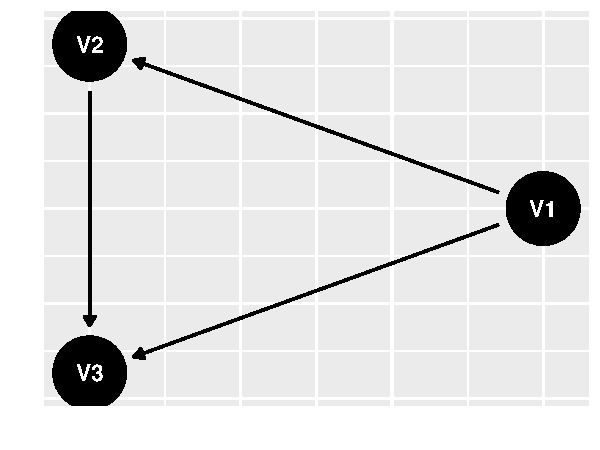
\includegraphics[width=\maxwidth]{./figures/grafo1-1} 

}

\caption[Exemplo de grafo]{Exemplo de grafo.}\label{fig:grafo1}
\end{figure}

\end{knitrout}

Grafos direcionados serão úteis para 
representar causalidade pois 
seus vértices serão variáveis e
suas arestas irão apontar de 
cada causa imediata para seu efeito.
Por exemplo, no \Cref{cap:intro}
consideramos um caso em que Sexo e Tratamento são
causas imediatas de recuperação e, além disso,
Sexo é causa imediata de Tratamento.
O grafo na \cref{fig:grafo1} poderia
representar estas relações se definirmos que
$V_1$ é Sexo, $V_2$ é Tratamento e 
$V_3$ é Recuperação.

Usando a representação de um grafo,
podemos imaginar caminhos sobre ele.
Um \textbf{caminho direcionado} inicia-se 
em um determinado vértice e, 
seguindo a direção das setas, 
vai de um vértice para outro.
Por exemplo, $(V_1, V_2, V_3)$ é
um caminho direcionado na 
\cref{fig:grafo1}, pois existe
uma seta de $V_1$ para $V_2$ e
de $V_2$ para $V_3$.
É comum denotarmos este caminho direcionado por
$V_1 \rightarrow V_2 \rightarrow V_3$.
Similarmente, $(V_1, V_3, V_2)$ não é
um caminho direcionado, pois
não existe seta de $V_3$ para $V_2$.
A definição de caminho direcionado é
formalizada a seguir:

\begin{definition}
 \label{lem:caminhodir}
 Um \textbf{caminho direcionado} é 
 uma sequência de vértices em
 um grafo direcionado,
 $C = \{C_1, \ldots, C_n\}$ tal que, 
 para cada $1 \leq i < n$,
 $(C_i, C_{i+1}) \in \sE$.
\end{definition}

\begin{definition}
 \label{def:descendente}
 Dizemos que $V_2$ é descendente de $V_1$ se
 existe um caminho direcionado de $V_1$ em $V_2$.
\end{definition}

Um \textit{caminho} é uma generalização 
de caminho direcionado.
Em um caminho, começamos em um vértice e,
seguindo por setas, mas 
não necessariamente na direção 
em que elas apontam, vamos
de um vértice para outro.
Por exemplo, na \cref{fig:grafo1}
vimos que $(V_1, V_3, V_2)$ não é um 
caminho direcionado pois não existe seta de $V_3$ para $V_2$.
Contudo, $(V_1, V_3, V_2)$ é um caminho pois
existe uma seta ligando $V_3$ e $V_2$,
a seta que aponta de $V_2$ para $V_3$.
É comum representarmos este caminho por
$V_1 \rightarrow V_3 \leftarrow V_2$.
Caminho é formalizado a seguir:

\begin{definition}
 \label{def:caminho}
 Um \textbf{caminho} é uma sequência de vértices,
 $C = \{C_1, \ldots, C_n\}$ tal que, 
 para cada $1 \leq i < n$,
 $(C_i, C_{i+1}) \in \sE$ ou 
 $(C_{i+1}, C_{i}) \in \sE$. 
 $(V_i, V_{i+1}) \in \sE$ ou 
 $(V_{i+1}, V_{i}) \in \sE$. 
\end{definition}

\subsection{Grafo Direcionado Acíclico (DAG)}

Um DAG é um grafo direcionado tal que,
para todo vértice, $V$, não é possível
seguir setas partindo de $V$ e
voltar para $V$. Este conceito é
formalizado a seguir:

\begin{definition}
 \label{def:dag}
 Um \textbf{grafo direcionado acíclico} (DAG) é
 um grafo direcionado, $\sG = (\sV, \sE)$,
 tal que, para todo
 vértice, $V \in \sV$, não existe um
 caminho direcionado, $C = \{C_1, \ldots, C_n\}$
 tal que $C_1 = V = C_n$.
\end{definition}

Usualmente representaremos
as relações causais por meio de um DAG.
Especificamente, existirá uma aresta de $V_1$ para $V_2$
para indicar que $V_1$ é causa imediata de $V_2$.
Caso um grafo direcionado não seja um DAG,
então existe um caminho de $V$ em $V$, isto é,
$V$ seria uma causa de si mesma, 
o que desejamos evitar.

Um DAG induz uma \textit{ordem parcial} entre 
os seus vértices. Isto é,
se existe uma aresta de $V_1$ para $V_2$,
então podemos interpretar que
$V_1$ antecede $V_2$ causalmente.
Com base nesta ordem parcial, é
possível construir diversas
definições que nos serão úteis.

Dizemos que $V_1$ é pai de $V_2$ em
um DAG, $\sG$, se
existe uma aresta de $V_1$ a $V_2$,
isto é, $(V_1, V_2) \in \sE$.
Denotamos por $Pa(V)$ o
conjunto de todos os pais de $V$:

\begin{definition}
 \label{def:pais}
 O conjunto de \textbf{pais} de $V \in \sV$ 
 em um DAG, $\sG = (\sV, \sE)$, é:
 $$Pa(V) := \{V^* \in \sV: (V^*, V) \in \sE\}.$$
\end{definition}

Similarmente, dizemos que $V_1$ é um ancestral de $V_2$ em
um DAG, se $V_1$ antecede $V_2$ causalmente. Isto é,
se $V_1$ é pai de $V_2$ ou, pai de pai de $V_2$, ou
pai de pai de pai de $V_2$, e assim por diante $\ldots$
Denotamos por $Anc(\V)$ o conjunto de 
todos os ancestrais de elementos de $\V$:

\begin{definition}
 \label{def:ancestrais}
 Em um DAG, $\sG = (\sV, \sE)$,
 o conjunto de \textbf{ancestrais} de $\V \subseteq \sV$, 
 $Anc(\V)$, é tal que
 $Anc(\V) \subseteq \sV$ e
 $V^* \in Anc(\V)$ se e somente se existe
 $V \in \V$ e
 um caminho direcionado, C, tal que
 $C_1 = V^*$ e $C_i = V$.
\end{definition}

Note que podemos interpretar $Anc(\V)$ como
o conjunto de todas as causas diretas e indiretas de $\V$.

Finalmente, diremos que um conjunto de vértices,
$\sA \subseteq \sV$ é \textit{ancestral} em um DAG,
se não existe algum vértice fora de $\sA$ que
seja pai de algum vértice em $\sA$.
Segundo nossa interpretação causal,
$\sA$ será ancestral quando 
nenhum vértice fora de $\sA$ 
é causa direta de 
algum vértice em $\sA$:

\begin{definition}
 \label{def:ancestral}
 Dizemos que $\sA \subseteq \sV$ é 
 \textbf{ancestral} em um DAG se,
 para todo vértice $V \in \sA$, temos que
 $Pa(V) \subseteq \sA$.
\end{definition}

\begin{lemma}
 \label{lem:anc}
 Em um DAG, $\sG$,
 para todo $\V \subseteq \sV$, 
 $Anc(\V)$ é ancestral.
\end{lemma}

\subsection{Modelo Probabilístico em um DAG}

Um modelo probabilístico em um DAG é
tal que cada um dos vértices é uma variável aleatória.
O DAG será usado para descrever 
relações de independência condicional existentes entre
estas variáveis.
Mais especificamente, cada vértice será
independente dos demais vértices dados os seus pais.
Uma maneira alternativa de pensar sobre esta afirmação é
imaginar que cada vértice é gerado somente pelos seus pais.
Esta intuição é formalizada em \cref{def:compativel}:

\begin{definition}
 \label{def:compativel}
 Para $\sV$ um conjunto de variáveis aleatórias,
 dizemos que uma função de densidade sobre $\sV$, 
 $f$, é compatível com um DAG, $\sG$, se:
 $$f(v_1,\ldots,v_n) = \prod_{i=1}^n f(v_i|Pa(v_i))$$
\end{definition}

Na prática, pode ser difícil verificar 
se a \cref{def:compativel} está satisfeita 
Para esses casos,
pode ser útil aplicar o 
\cref{lem:compativel-equiv}:

\begin{lemma}
 \label{lem:compativel-equiv}
 Uma função de densidade, $f$, é
 compatível com um DAG, $\sG$,
 se e somente se, existem funções,
 $g_1,\ldots,g_n$ tais que:
 $$f(v_1,\ldots,v_n) = \prod_{i=1}^n g_i(v_i, Pa(v_i))$$
\end{lemma}

O seguinte lema também é útil

\begin{lemma}
 \label{lem:anc_fat}
 Seja $\sG = (\sV, \sE)$ um DAG.
 Se $\sA$ é ancestral e 
 $f$ é compatível com $\sG$, então
 \begin{align*}
  f(\sA) = \prod_{V \in \sA} f(V|Pa(V))
 \end{align*}
\end{lemma}

A seguir, estudaremos três tipos fundamentais
de modelos probabilísticos em DAG's com
$3$ vértices. 
A intuição obtida a partir destes
exemplos continuará valendo quando
estudarmos grafos mais gerais.

\subsection{Exemplos de Modelo Probabilístico em um DAG}
\label{sec:dag-ex}

Nos exemplos a seguir, considere que
$\sV = (V_1, V_2, V_3)$.

\subsubsection{Confundidor (Confounder)}

No modelo de confundidor, 
as únicas duas arestas são 
$(V_2, V_1)$ e $(V_2, V_3)$.
Uma ilustração de um confundidor
pode ser encontrada 
na \cref{fig:confundidor}.
O modelo de confundidor pode ser usado quando
acreditamos que $V_2$ é uma causa comum a
$V_1$ e a $V_3$. Além disso,
$V_1$ não é causa imediata de $V_3$ 
nem vice-versa.

\begin{knitrout}
\definecolor{shadecolor}{rgb}{0.969, 0.969, 0.969}\color{fgcolor}\begin{figure}[t]

{\centering 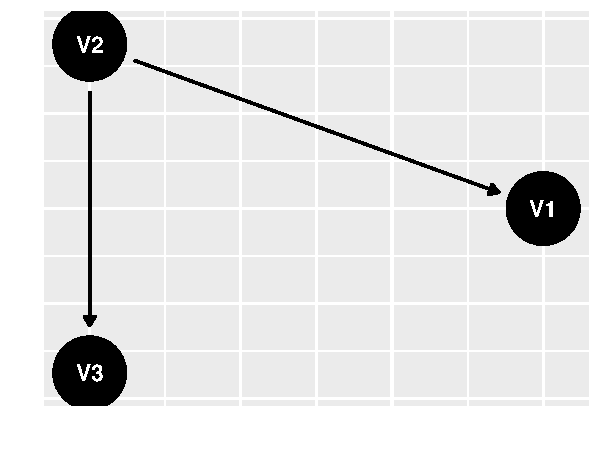
\includegraphics[width=\maxwidth]{./figures/confundidor-1} 

}

\caption[Ilustração de confundidor]{Ilustração de confundidor.}\label{fig:confundidor}
\end{figure}

\end{knitrout}

Em um modelo de confundidor 
a relação de dependência entre 
$V_1$ e $V_3$ é explicada pelos
resultados a seguir:

\begin{lemma}
 \label{lem:conf-ind}
 Para qualquer probabilidade compatível com 
 o DAG na \cref{fig:confundidor},
 $V_1 \ind V_3 | V_2$.
\end{lemma}

\begin{proof}
 \begin{align*}
  f(v_1,v_3|v_2) 
  &= \frac{f(v_1,v_2,v_3)}{f(v_2)} \\
  &= \frac{f(v_2)f(v_1|v_2)f(v_3|v_2)}{f(v_2)} 
  & \text{\cref{def:compativel}} \\
  &= f(v_1|v_2)f(v_3|v_2)
 \end{align*}
\end{proof}

\begin{lemma}
 \label{lem:conf-dep}
 Existe ao menos uma probabilidade compatível com
 o DAG na \cref{fig:confundidor} tal que
 $V_1 \not\ind V_3$.
\end{lemma}

\begin{proof}
 Considere que $V_2 \sim \text{Bernoulli}(0.02)$.
 Além disso, $V_1, V_3 \in \{0,1\}$ são independentes dado $V_2$. 
 Também,
 $\P(V_1 = 1|V_2 = 1) = \P(V_3 = 1|V_2 = 1) = 0.9$ e
 $\P(V_1 = 1|V_2 = 0) = \P(V_3 = 1|V_2 = 0) = 0.05$.
 Note que, por construção, $\P$ é 
 compatível com \cref{fig:confundidor}.
 Isto é, $P(v_1,v_2,v_3) = \P(v_2)\P(v_1|v_2)\P(v_3|v_2)$.
 Além disso,
 \begin{align*}
  \P(V_1 = 1) &= \P(V_1 = 1, V_2 = 1) + \P(V_1 = 1, V_2 = 0) \\
              &= \P(V_2=1)\P(V_1=1|V_2=1)
               +\P(V_2=0)\P(V_1=1|V_2=0) \\
              &= 0.02 \cdot 0.9 + 0.98 \cdot 0.05= 0.067
 \end{align*}
 Por simetria, $\P(V_3=1) = 0.067$. Além disso,
 \begin{align*}
  \P(V_1 = 1, V_3 = 1)
  &= \P(V_1 = 1, V_3 = 1, V_2 = 1) 
  +  \P(V_1 = 1, V_3 = 1, V_2 = 0) \\
  &= \P(V_2 = 1)\P(V_1 = 1|V_2 = 1)\P(V_3 = 1|V_2 = 1)
  +  \P(V_2 = 0)\P(V_1 = 1|V_2 = 0)\P(V_3 = 1|V_2 = 0) \\
  &= 0.02 \cdot 0.9 \cdot 0.9 + 0.98 \cdot 0.05 \cdot 0.05 = 0.01865
 \end{align*}
 Como $\P(V_1=1)\P(V_3=1) = 0.067 \cdot 0.067 \approx 0.0045 \neq 0.01865 = \P(V_1=1,V_3=1)$,
 temos que $V_1$ e $V_3$ não são independentes.
\end{proof}

Combinando os \cref{lem:conf-ind,lem:conf-dep} é 
possível compreender melhor como 
usaremos confundidores num contexto causal.
Nestes casos, $V_2$ será uma causa comum a $V_1$ e a $V_3$.
Esta causa comum torna $V_1$ e $V_3$ associados,
ainda que nenhum seja causa direta ou indireta do outro.

Podemos contextualizar estas ideias
em um caso de diagnóstico de dengue.
Considere que 
$V_2$ é a indicadora de que um indivíduo tem dengue, e
$V_1$ e $V_3$ são indicadoras de sintomas típicos de dengue, como
dor atrás dos olhos e febre.
Neste caso, $V_1$ e $V_3$ tipicamente são associados:
caso um paciente tenha febre,
aumenta a probabilidade de que tenha dengue e, portanto,
aumenta a probabilidade de que tenha dor atrás dos olhos.
Contudo, apesar dessa associação 
$V_3$ não tem influência causal sobre $V_1$.
Se aumentarmos a temperatura corporal do indivíduo,
não aumentará a probabilidade de que ele tenha dor atrás dos olhos.
A dengue que causa febre, não o contrário.

\subsubsection{Cadeia (Chain)}

No modelo de cadeia, 
as únicas duas arestas são 
$(V_1, V_2)$ e $(V_2, V_3)$.
Uma ilustração de uma cadeia
pode ser encontrada 
na \cref{fig:cadeia}.
Neste modelo, acreditamos que 
$V_1$ é causa de $V_2$ que,
por sua vez, é causa de $V_3$.
Assim, $V_1$ é ancestral de $V_3$,
isto é, o primeiro é 
causa indireta do segundo.


\begin{knitrout}
\definecolor{shadecolor}{rgb}{0.969, 0.969, 0.969}\color{fgcolor}\begin{figure}[t]

{\centering 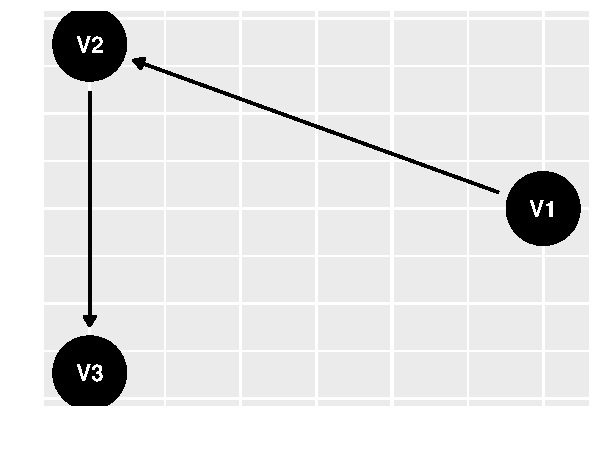
\includegraphics[width=\maxwidth]{./figures/cadeia-1} 

}

\caption[Ilustração de cadeia]{Ilustração de cadeia.}\label{fig:cadeia}
\end{figure}

\end{knitrout}

Em um modelo de cadeia 
a relação de dependência entre 
$V_1$ e $V_3$ é explicada pelos
resultados a seguir:

\begin{lemma}
 \label{lem:med-ind}
 Para qualquer probabilidade compatível com 
 o DAG na \cref{fig:cadeia},
 $V_1 \ind V_3 | V_2$.
\end{lemma}

\begin{proof}
 \begin{align*}
  f(v_3|v_1,v_2) 
  &= \frac{f(v_1,v_2,v_3)}{f(v_1,v_2)} \\
  &= \frac{f(v_1)f(v_2|v_1)f(v_3|v_2)}{f(v_1)f(v_2|v_1)} 
  & \text{\cref{def:compativel}} \\
  &= f(v_3|v_2)
 \end{align*}
\end{proof}

\begin{lemma}
 \label{lem:med-dep}
 Existe ao menos uma probabilidade compatível com
 o DAG na \cref{fig:cadeia} tal que
 $V_1 \not\ind V_3$.
\end{lemma}

\begin{proof}
 Considere que $V_1 \sim \text{Bernoulli}(0.5)$,
 $\P(V_2=1|V_1=1)=0.9$, $\P(V_2=1|V_1=0)=0.05$,
 $\P(V_3=1|V_2=1,V_1)=0.9$, e $\P(V_3=1|V_2=0,V_1)=0.05$.
 Note que $(V_1,V_2,V_3)$ formam uma Cadeia de Markov.
 Note que, por construção, $\P$ é 
 compatível com \cref{fig:cadeia}.
 Isto é, $P(v_1,v_2,v_3) = \P(v_1)\P(v_2|v_1)\P(v_3|v_2)$.
 Além disso,
 \begin{align*}
  \P(V_3 = 1) &= \P(V_1=0, V_2=0, V_3=1) + \P(V_1=0, V_2=1, V_3=1) \\
              &+ \P(V_1=1, V_2=0, V_3=1) + \P(V_1=1, V_2=1, V_3=1) \\
              &= 0.5 \cdot 0.9 \cdot 0.05 + 0.5 \cdot 0.05 \cdot 0.9 \\
              &+ 0.5 \cdot 0.05 \cdot 0.05 + 0.5 \cdot 0.9 \cdot 0.9 
              = 0.45125
 \end{align*}
 Além disso,
 \begin{align*}
  \P(V_1 = 1, V_3 = 1)
  &= \P(V_1 = 1, V_2 = 0, V_3 = 1) 
  +  \P(V_1 = 1, V_2 = 1, V_3 = 1) \\
  &= 0.5 \cdot 0.05 \cdot 0.9 + 0.5 \cdot 0.9 \cdot 0.9
  = 0.40625
 \end{align*}
 Como $\P(V_1=1)\P(V_3=1) = 0.5 \cdot 0.45125 \approx 0.226 \neq 
 0.40625 = \P(V_1=1,V_3=1)$,
 temos que $V_1$ e $V_3$ não são independentes.
\end{proof}

Combinando os \cref{lem:med-ind,lem:med-dep} é 
possível compreender melhor como 
usaremos cadeias num contexto causal.
Nestes casos, $V_2$ será uma consequência de $V_1$ e
uma causa de $V_3$. Assim, a cadeia torna
$V_1$ e $V_3$ e associados, 
ainda que nenhum seja causa direta do outro.
Contudo, ao contrário do confundidor,
neste caso $V_1$ é uma causa indireta de $V_3$,
isto é, tem influência causal sobre $V_3$.

Para contextualizar estas ideias,
considere que $V_1$ é a indicadora de consumo elevado de sal,
$V_2$ é a indicadora de pressão alta, e
$V_3$ é a indicadora de ocorrência de um derrame.
Como consumo elevado de sal causa pressão alta e
pressão alta tem influência causal sobre a ocorrência de um derrame,
pressão alta é uma cadeia que é
um mediador entre consumo elevado de sal e
ocorrência de derrame. Assim,
consumo elevado de sal tem influência causal sobre
a ocorrência de derrame.

\subsubsection{Colisor (Collider)}

O último exemplo de DAG com $3$ vértices que 
estudaremos é o de modelo de colisor, em que
as únicas duas arestas são 
$(V_1, V_2)$ e $(V_3, V_2)$.
Uma ilustração de um colisor
pode ser encontrada 
na \cref{fig:colisor}.
O modelo de colisor pode ser usado quando
acreditamos que $V_1$ e $V_3$ são 
causas comuns a $V_2$. Além disso,
$V_1$ não é causa imediata de $V_3$ 
nem vice-versa.

\begin{knitrout}
\definecolor{shadecolor}{rgb}{0.969, 0.969, 0.969}\color{fgcolor}\begin{figure}[t]

{\centering 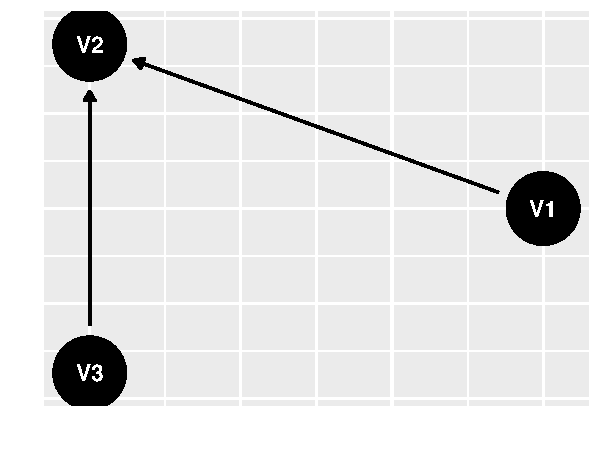
\includegraphics[width=\maxwidth]{./figures/colisor-1} 

}

\caption[Ilustração de colisor]{Ilustração de colisor.}\label{fig:colisor}
\end{figure}

\end{knitrout}

Em um modelo de colisor 
a relação de dependência entre 
$V_1$ e $V_3$ é explicada pelos
resultados a seguir:

\begin{lemma}
 \label{lem:col-ind}
 Para qualquer probabilidade compatível com 
 o DAG na \cref{fig:colisor},
 $V_1 \ind V_3$.
\end{lemma}

\begin{proof}
 \begin{align*}
  f(v_1,v_3) 
  &= \int f(v_1, v_2, v_3) dv_2 \\
  &= \int f(v_1)f(v_3)f(v_2|v_1,v_3) dv_2 
  & \text{\cref{def:compativel}} \\
  &= f(v_1)f(v_3) \int f(v_2|v_1,v_3) dv_2 \\
  &= f(v_1)f(v_3)
 \end{align*}
\end{proof}

\begin{lemma}
 \label{lem:col-dep}
 Existe ao menos uma probabilidade compatível com
 o DAG na \cref{fig:colisor} tal que
 $V_1 \not\ind V_3 | V_2$.
\end{lemma}

\begin{proof}
 Considere que $V_1$ e $V_3$ são
 independentes e tem distribuição $\text{Bernoulli}(0.5)$.
 Além disso, $V_2 \equiv V_1+V_3$.
 Como $\P(V_3 = 1) = 0.5$ e
 $\P(V_3=1|V_1=1,V_2=2) = 1$, conclua que
 $V_1 \not\ind V_3 | V_2$.
\end{proof}

Combinando os \cref{lem:col-ind,lem:col-dep} vemos 
como utilizaremos confundidores num contexto causal.
Nestes casos, $V_1$ e $V_3$ serão causas comuns e independentes de $V_2$.
Uma vez que obtemos informação sobre o efeito comum, $V_2$,
$V_1$ e $V_3$ passam a ser associados.

Esse modelo pode ser contextualizado observando
a prevalência de doenças em uma determinada população 
\citep{Sackett1979}.
Considere que  $V_1$ e $V_3$ são 
indicadoras de que um indivíduo tem
doenças que ocorrem independentemente na população.
Além disso, $V_2$ é a indicadora de que 
o indíviduo foi hospitalizado, isto é,
$V_2$ é influeciado causalmente 
tanto por $V_1$ quanto por $V_3$.
Para facilitar as contas envolvidas,
desenvolveremos o exemplo com distribuições fictícias.
Considere que
$V_1$ e $V_3$ são independentes e
tem distribuição Bernoulli(0.05).
Além disso, quanto maior o número de doenças,
maior a probabilidade de o indíviduo ser hospitalizado.
Por exemplo,
$\P(V_2=1|V_1=0,V_3=0) = 0.01$,
$\P(V_2=1|V_1=0,V_3=1) = 0.1$,
$\P(V_2=1|V_1=1,V_3=0) = 0.1$, e
$\P(V_2=1|V_1=1,V_3=1) = 0.5$.

Com base nestas especificações, podemos
verificar se $V_1$ e $V_3$ estão associados
quando $V_2=1$. Para tal,
primeiramente calcularemos algumas
probabilidades conjuntas que serão úteis:
\begin{align}
 \label{eq:ex-col-1}
 \begin{cases}
  \P(V_1=0,V_2=1,V_3=0) &= 0.95 \cdot 0.01 \cdot 0.95 = 0.009025 \\
  \P(V_1=0,V_2=1,V_3=1) &= 0.95 \cdot 0.1 \cdot 0.05 = 0.0475 \\
  \P(V_1=1,V_2=1,V_3=0) &= 0.05 \cdot 0.1 \cdot 0.95 = 0.0475 \\
  \P(V_1=1,V_2=1,V_3=1) &= 0.05 \cdot 0.5 \cdot 0.05 = 0.00125
 \end{cases}
\end{align}

Com base nestes cálculos é possível obter
a prevalência da doença dentre os indivíduos hospitalizados:
\begin{align*}
 \P(V_1=1|V_2=1) 
 &= \frac{\P(V_1=1,V_2=1)}{\P(V_2=1)} \\
 &= \frac{0.0475 + 0.00125}{0.009025 + 0.0475 + 0.0475 + 0.00125} 
 & \text{\cref{eq:ex-col-1}} \\
 &\approx 0.46
\end{align*}

Finalmente,
\begin{align*}
 \P(V_1 = 1|V_2 = 1, V_3 = 1)
 &= \frac{\P(V_1=1,V_2=1,V_3=1)}{\P(V_2=1,V_3=1)} \\
 &= \frac{\P(V_1=1,V_2=1,V_3=1)}
 {\P(V_1=0,V_2=1,V_3=1) + \P(V_1=1,V_2=1,V_3=1)} \\
 &= \frac{0.00125}{0.0475 + 0.00125} & \text{\cref{eq:ex-col-1}} \\
 &\approx 0.26 
\end{align*}

Como $\P(V_1=1|V_2=1) = 0.46 \neq 0.26 \approx \P(V_1=1|V_2=1,V_3=1)$,
verificamos que $V_1$ não é independente de $V_3$ dado $V_2$.
De fato, ao observar que um indivíduo está hospitalizado e
tem uma das doenças, a probabilidade de que ele tenha
a outra doença é inferior àquela obtida se soubéssemos apenas
que o indivíduo está hospitalizado.

Esta observação 
não implica que uma doença tenha influência causal sobre a outra.
Note que a frequência de hospitalização aumenta 
drasticamente quando um indivíduo tem ao menos uma das doenças.
Além disso, cada uma das doenças é relativamente rara na população geral.
Assim, dentre os indíviduos hospitalizados,
a frequência daqueles que tem somente uma das doenças é
maior do que seria caso as doenças não estivessem associadas.
Quando fixamos o valor de uma consequência comum (hospitalização),
as causas (doenças) passam a ser associadas.
Esta associação não significa que
infectar um indivíduo com uma das doenças
reduz a probabilidade que ele tenha a outra.

\subsection{Modelo Estrutural Causal (Structural Causal Model)}

Com base nos conceitos abordados anteriormente,
finalmente podemos definir formalmente
o Modelo Estrutural Causal (SCM):

\begin{definition}
 \label{def:scm}
 Um SCM é um par $(\sG,f)$ tal que
 $\sG = (\sV, \sE)$ é um DAG (\cref{def:dag}) e
 $f$ é uma função de densidade sobre $\sV$
 compatível com $\sG$ (\cref{def:compativel}).
 Neste caso, é comum chamarmos $\sG$ de
 \textbf{grafo causal} do SCM $(\sG,f)$.
\end{definition}

Note pela \cref{def:scm} que
um SCM é formalmente um modelo probabilístico em um DAG.
O principal atributo de um SCM que 
o diferencia de um modelo probabilístico genérico em um DAG é
como o interpretamos.
Existe uma aresta de $V_1$ em $V_2$ em um SCM
se e somente se $V_1$ é uma causa direta de $V_2$.

\begin{definition}
 Dizemos que $(\sG,f)$ é um SCM linear Gaussiano se,
 existe matriz diagonal positiva, $\Sigma$, e
 $\beta in \Re^{n \times n}$ tal que,
 para todo vértice $V_i$,
 $\beta_{i,j} = 0$ quando $V_j \notin Pa(V_i)$ e
 \begin{align*}
  V_i|Pa(V) &\sim N(\beta_i, \Sigma_{i,i})
 \end{align*}
\end{definition}

\begin{lemma}
 Se $(\sG,f)$ é um SCM linear Gaussiano, então
 $\sV \sim N(0, (I-\beta)^{-1}\Sigma((I-\beta)^{-1})^t)$.
 
\end{lemma}

No próximo capítulo estudaremos consequências desta interpretação causal.
Contudo, antes disso, a próxima seção desenvolverá
um resultado fundamental de modelos probabilísticos em DAGs que
será fundamental nos capítulos posteriores.

\subsection{Exercícios}

\begin{exercise}
 Em um DAG, $\sG = (\sV, \sE)$,
 Considere que $Anc^*(\V) \subseteq \sV$ é
 definido como o menor conjunto tal que
 $\V \subseteq Anc^*(\V)$ e,
 se $V \in Anc^*(\V)$, então
 $Pa(V) \subseteq Anc^*(\V)$.
 Prove que $Anc(\V) \equiv Anc^*(\V)$.
\end{exercise}

\begin{exercise} 
 Prove o \cref{lem:anc}.
\end{exercise}

\begin{exercise}
 \label{lemma:anc_fact}
 Prove que se $\Z$ é ancestral, então
 $f(\Z) = \prod_{Z \in \Z}f(Z|Pa(Z))$. 
\end{exercise}

\begin{exercise}
 Sejam $\sG_1 = (\sV, \sE_1)$ e
 $\sG_2 = (\sV, \sE_2)$ grafos
 tais que $\sE_1 \subseteq \sE_2$.
 Prove que se 
 $f$ é compatível com $\sG_2$, então 
 $f$ é compatível com $\sG_1$.
\end{exercise}

\begin{exercise}
 Prove o \cref{lem:compativel-equiv}.
\end{exercise}

\begin{exercise}
 Prove o \cref{lem:anc_fat}.
\end{exercise}

\begin{exercise}
 Considere que $(X_1,X_2)$ são independentes e
 tais que $\P(X_i=1)=\P(X_i=-1)=0.5$.
 Além disso, $Y \equiv X_1 \cdot X_2$.
 \begin{enumerate}[label=(\alph*)]
  \item Desenhe um DAG compatível
  com as relações de independência dadas pelo enunciado.
  \item Prove que $Y$ e $X_1$ são independentes.
  Isso contradiz sua resposta para o item anterior?
 \end{enumerate}
\end{exercise}

\begin{exercise}
 Para cada um dos modelos de confundidor, cadeia e colisor,
 dê exemplos de situações práticas em que este modelo é razoável.
\end{exercise}

\begin{exercise}
 Considere que, dado $T$, $X_1,\ldots,X_n$ são i.i.d. e
 $X_i|T \sim \text{Bernoulli}(T)$. Além disso,
 $T \sim \text{Beta}(a,b)$.
 \begin{enumerate}[label=(\alph*)]
  \item Seja $f(t,x_1,\ldots,x_n)$ dada pelo enunciado.
  Exiba um DAG, $\sG$, tal que $f$ é compatível com $\sG$.
  \item $(X_1,\ldots,X_n)$ são independentes?
  \item Determine $f(x_1,\ldots,x_n)$.
 \end{enumerate}
\end{exercise}

\begin{exercise}
 Exiba um exemplo em que $V_1$, $V_2$, $V_3$ sejam binárias,
 que $V_2$ seja um colisor e que, além disso,
 $Corr[V_1,V_3|V_2=1] > 0$.
\end{exercise}

\begin{exercise}
 Seja $\sV = (V_1, V_2, V_3)$
 Exiba um exemplo de $f$ sobre $\sV$ e
 grafos $\sG_1$ e $\sG_2$ sobre $\sV$ tais que
 $\sG_1 \neq \sG_2$ e
 $f$ é compatível tanto com $\sG_1$ 
 quanto com $\sG_2$.
\end{exercise}

\begin{exercise}
 Seja $f$ uma densidade arbitrária sobre $\sV = (V_1,\ldots,V_n)$.
 Exiba um DAG sobre $\sV$, $\sG$,
 tal que $f$ é compatível com $\sG$.
\end{exercise}

\begin{exercise}
 Exiba um exemplo em que $V_2$ é um colisor 
 entre $V_1$ e $V_2$, 
 $V_4$ tem como único pai $V_2$ e
 $V_1$ e $V_3$ são dependentes dado $V_4$.
\end{exercise}

\section{Independência Condicional e D-separação}
\label{sec:d-sep}

Independência condicional é uma forma fundamental de
indicar relações entre variáveis aleatórias.
Se $\X_1,\ldots,\X_d$ e $\Y$ são vetores de variáveis aleatórias,
definimos que $(\X_1,\ldots,\X_d) | \Y$, isto é,
$\X_1,\ldots,\X_d$ são independentes dado $\Y$, se
conhecido o valor de $\Y$, 
observar quaisquer valores de $\X$ não traz 
informação sobre os demais valores.
Nesta seção veremos que 
as relações de independência condicional em um SCM
estão diretamente ligadas ao seu grafo.

\subsection{Independência Condicional}
\label{sec:indep}

\begin{definition}
 \label{def:indep}
 Dizemos que $(\X_1,\ldots,\X_d)$ são independentes dado $\Y$ se,
 para qualquer $\x_1,\ldots,\x_n$ e $\y$,
 \begin{align*}
  f(\x_1,\ldots,\x_n|\y)	&= \prod_{i=1}^d f(\x_i|\y)
 \end{align*}
 Em particular, $(\X_1,\ldots,\X_d)$ são independentes se,
 para quaiquer $(\x_1,\ldots,\x_d)$,
 \begin{align*}
  f(\x_1,\ldots,\x_d)	&= \prod_{i=1}^d f(\x_i)
 \end{align*}
\end{definition}

Verificar se a \cref{def:indep} está satisfeita nem sempre é fácil.
A princípio, ela exige obter tanto a distribuição condicional conjunta, 
$f(\x_1,\ldots,\x_d|\y)$, quanto cada uma das marginais, $f(\x_i|\y)$.
O \cref{lemma:equivIndep} a seguir apresenta outras condições que
são equivalentes a independência condicional:

\begin{lemma}
 \label{lemma:equivIndep}
 As seguintes afirmações são equivalentes:
 \begin{enumerate}
  \item $(\X_1,\ldots,\X_d)$ são independentes dado $\Y$,
  \item Existem funções, $h_1,\ldots,h_d$ tais que
  $f(\x_1,\ldots,\x_d|\y) = \prod_{j=1}^{d}{h_j(\x_j,\y)}$.	
	\item Para todo $i$, 
	$f(\x_i|\x_{-i},\y) = f(\x_i|\y)$.
	\item Para todo $i$,
	$f(\x_i|\x_1^{i-1},\y) = f(\x_i|\y)$.
 \end{enumerate}
\end{lemma}

As condições no \cref{lemma:equivIndep} são, em geral,
mais fáceis de verificar do que 
a definição direta de independência condicional.
A seguir veremos que, em um SMC, pode
ser mais fácil ainda verificar
muitas das relações de independência condicional.

\subsection{D-separação}

Em um SCM, é possível indicar 
as relações de independência incondicional em $\sV$
por meio do grafo associado.
Intuitivamente, haverá uma dependência
entre $V_1$ e $V_2$ se for possível
transmitir a informação de $V_1$ para $V_2$
por um caminho que ligue ambos os vértices.
Para entender se a informação 
pode ser transmitida por um caminho,
classificaremos a seguir os vértices que o constituem.

\begin{definition}
 \label{def:caminho-cat}
 Seja $C = (C_1,\ldots,C_n)$ um caminho 
 em um DAG, $\sG = (\sV,\sE)$.
 Para cada $2 \leq i \leq n-1$:
 \begin{enumerate}
  \item $C_i$ é um \textbf{confundidor} em $C$ se
  $(C_i,C_{i-1}) \in \sE$ e $(C_i,C_{i+1}) \in \sE$,
  isto é, existem arestas apontando de $C_i$ para
  $C_{i-1}$ e $C_{i+1}$. Neste caso, desenhamos
  $C_{i-1} \leftarrow C_i \rightarrow C_{i+1}$.
  \item $C_i$ é uma \textbf{cadeia} em $C$ se
  $(C_{i-1},C_{i}) \in \sE$ e $(C_i,C_{i+1}) \in \sE$, ou
  $(C_{i+1},C_{i}) \in \sE$ e $(C_i,C_{i-1}) \in \sE$,
  isto é, $(C_{i-1},C_i,C_{i+1})$ ou $(C_{i+1},C_i,C_{i-1})$ é 
  um caminho direcionado. Neste caso, desenhamos
  $C_{i-1} \rightarrow C_i \rightarrow C_{i+1}$ ou
  $C_{i-1} \leftarrow C_i \leftarrow C_{i+1}$.
  \item $C_i$ é um \textbf{colisor} em $C$ se
  $(C_{i-1},C_{i}) \in \sE$ e $(C_{i+1},C_{i}) \in \sE$,
  isto é, existem arestas apontando de $C_{i-1}$ e de $C_{i+1}$ 
  para $C_{i}$. Neste caso, desenhamos
  $C_{i-1} \rightarrow C_i \leftarrow C_{i+1}$.
 \end{enumerate}
\end{definition}

Note que a classificação na \cref{def:caminho-cat}
generaliza os exemplos de DAG's com 3 vértices 
na \cref{sec:dag-ex}. 

Essa classificação é ilustrada com 
o DAG na \cref{fig:caminho-cat}.
Existem dois caminhos que vão de $V_1$ a $V_4$:
$V_1 \rightarrow V_2 \leftarrow V_4$ e
$V_1 \rightarrow V_2 \rightarrow V_3 \leftarrow V_4$.
No primeiro caminho $V_2$ é um colisor, pois
o caminho passa por duas arestas que apontam para $V_2$.
Já no segundo caminho $V_2$ é uma cadeia e
$V_3$ é um colisor.
Note que a classificação do vértice depende 
do caminho analisado.
Enquanto que no primeiro caminho $V_2$ é um colisor,
no segundo $V_2$ é uma cadeia

\begin{knitrout}
\definecolor{shadecolor}{rgb}{0.969, 0.969, 0.969}\color{fgcolor}\begin{figure}[t]

{\centering 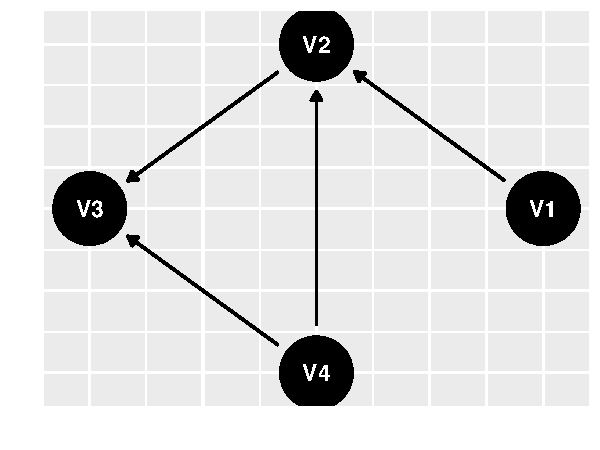
\includegraphics[width=\maxwidth]{./figures/caminho-cat-1} 

}

\caption[Ilustração do conceito de bloqueio de um caminho]{Ilustração do conceito de bloqueio de um caminho. No caminho (V1, V2, V4), V2 é um colisor. Isto ocorre pois, para chegar de V1 a V4 passando apenas por V2, as duas arestas apontam para V2. Já no caminho (V1, V2, V3, V4) temos que V2 é uma cadeia. Para chegar de V1 a V3 passando por V2, passa-se por duas arestas, uma entrando e outra saindo de V2. Como V2 é um colisor em (V1, V2, V4), este caminho está bloqueado se e somente se o valor de V2 é desconhecido. Como V2 é uma cadeia em (V1, V2, V3, V4), esse caminho está bloqueado quando o valor de V2 é conhecido.}\label{fig:caminho-cat}
\end{figure}

\end{knitrout}

Com base na \cref{def:caminho-cat}, é
possível compreender se um caminho permite a
passagem de informação.
Na \cref{sec:dag-ex} vimos que,
se $V_2$ é um confundidor ou uma cadeia entre
$V_1$ e $V_3$, então
$V_1$ e $V_3$ são independentes dado $V_2$.
Por analogia, podemos intuir que um vértice que
é um confundidor ou uma cadeia num caminho
não permite a passagem de informação
quando seu valor é conhecido.
Similarmente, na \cref{sec:dag-ex},
se $V_2$ é um colisor entre
$V_1$ e $V_3$, então 
$V_1$ e $V_3$ são independentes.
Assim, também podemos intuir que um vértice que
é um colisor em um caminho não permite
a passagem de informação quando seu valor é desconhecido.
Finalmente, a informação não passa pelo caminho quando
ela não passa por pelo menos um de seus vértices.
Neste caso, dizemos que o caminho está \textit{bloqueado}:

\begin{definition}
 \label{def:caminho-bloq}
 Seja $C = (C_1,\ldots,C_n)$ um caminho 
 em um DAG, $\sG = (\sV,\sE)$.
 Dizemos que $C$ está bloqueado dado $\Z \subset \sV$, se
 \begin{enumerate}
  \item Existe algum $2 \leq i \leq n-1$ tal que
  $C_i$ é um confundidor ou cadeia em $C$ e $C_{i} \in \Z$, ou
  \item Existe algum $2 \leq i \leq n-1$ tal que 
  $C_i$ é um colisor em $C$ e $C_{i} \notin Anc(\Z)$.
 \end{enumerate}
\end{definition}

Finalmente, dizemos que $\V_1$ está d-separado de $\V_2$
dado $\V_3$ se todos os caminhos de 
$\V_1$ a $\V_2$ estão bloqueados dado $\V_3$:

\begin{definition}
 \label{def:d-sep}
 Seja $\sG = (\sV, \sE)$ um DAG. 
 Para $\V_1,\V_2,\V_3 \subseteq \sV$, dizemos que
 $\V_1$ está d-separado de $\V_2$ dado $\V_3$ se,
 para todo caminho $C = (C_1,\ldots,C_n)$ tal que
 $C_1 \in V_1$ e $C_n \in \V_2$,
 $C$ está bloqueado dado $\V_3$.
 Neste caso, escrevemos $\V_1 \perp \V_2 | \V_3$.
\end{definition}

Intuitivamente, se $\V_1 \perp \V_2 | \V_3$, então 
não é possível passar informação de $\V_1$ a $\V_2$ quando
$\V_3$ é conhecido.
Assim, temos razão para acreditar que
$\V_1$ é condicionalmente independente de $\V_2$ dado $\V_3$,
isto é $\V_1 \ind \V_2 | \V_3$.
Esta conclusão é apresentada no 
\cref{thm:d-sep} a seguir:

\begin{theorem}
 \label{thm:d-sep}
 Seja $\sG = (\sV, \sE)$ um DAG e
 $\sV$ um conjunto de variáveis aleatórias.
 $\V_1$ está d-separado de $\V_2$ dado $\V_3$
 se e somente se, para todo $f$ compatível com $\sG$,
 $\V_1 \ind^f \V_2 | \V_3$.
\end{theorem}

\begin{example}
 \label{ex:dsep}
 Considere o DAG na \cref{fig:caminho-cat}.
 Para avaliar se $V_1$ e $V_3$ são d-separados,
 precisamos analisar todos os caminhos de um para o outro.
 Estes caminhos são: $V_1 \rightarrow V_2 \rightarrow V_3$, e
 $V_1 \rightarrow V_2 \leftarrow V_4 \rightarrow V_3$.
 No primeiro caminho $V_2$ é um confundidor e, assim,
 o caminho não está bloqueado marginalmente.
 Portanto, $V_1$ e $V_3$ não são d-separados marginalmente.
 Por outro lado, no segundo caminho $V_2$ é um colisor e
 $V_4$ é um confundidor. Assim,
 condicionando em $V_2$, este caminho não está bloqueado.
 Portanto, $V_1$ e $V_3$ não são d-separados dado $V_2$.
 Finalmente, dado $V_2$ e $V_4$, 
 ambos os caminhos estão bloqueados, 
 pois $V_2$ é um confundidor no primeiro e
 $V_4$ é um confundidor no segundo.
 Assim, $V_1$ e $V_3$ são d-separados dado $(V_2,V_4)$.
 Para treinar este raciocínio,
 continue analisando a d-separação entre $V_1$ e $V_4$.
 
 O algoritmo para testar d-separação está
 implementado em diversos pacotes.
 Além disso, é possível utilizar o
 \cref{thm:d-sep} para enunciar 
 todas as relações de independência condicional que
 são necessárias em um grafo.
 Estas implementações estão ilustradas abaixo:
\begin{knitrout}
\definecolor{shadecolor}{rgb}{0.969, 0.969, 0.969}\color{fgcolor}\begin{kframe}
\begin{alltt}
\hlcom{# Especificar o grafo}
\hlstd{grafo} \hlkwb{<-} \hlstr{"dag\{
   V1 -> V2 <- V4;
   V2 -> V3 <- V4
\}"}

\hlkwd{dseparated}\hlstd{(grafo,} \hlstr{"V1"}\hlstd{,} \hlstr{"V3"}\hlstd{,} \hlkwd{c}\hlstd{(}\hlstr{"V2"}\hlstd{))}
\end{alltt}
\begin{verbatim}
## [1] FALSE
\end{verbatim}
\begin{alltt}
\hlkwd{dseparated}\hlstd{(grafo,} \hlstr{"V1"}\hlstd{,} \hlstr{"V3"}\hlstd{,} \hlkwd{c}\hlstd{(}\hlstr{"V4"}\hlstd{))}
\end{alltt}
\begin{verbatim}
## [1] FALSE
\end{verbatim}
\begin{alltt}
\hlkwd{dseparated}\hlstd{(grafo,} \hlstr{"V1"}\hlstd{,} \hlstr{"V3"}\hlstd{,} \hlkwd{c}\hlstd{(}\hlstr{"V2"}\hlstd{,} \hlstr{"V4"}\hlstd{))}
\end{alltt}
\begin{verbatim}
## [1] TRUE
\end{verbatim}
\begin{alltt}
\hlkwd{impliedConditionalIndependencies}\hlstd{(grafo)}
\end{alltt}
\begin{verbatim}
## V1 _||_ V3 | V2, V4
## V1 _||_ V4
\end{verbatim}
\end{kframe}
\end{knitrout}
\end{example}

\begin{example}
 Considere que $\V_1$ e $\V_2$ 
 não são d-separados dado $\V_3$.
 O \cref{thm:d-sep} garante apenas que existe
 algum $f$ compatível com o DAG tal que
 $\V_1$ e $\V_2$ são 
 condicionalmente dependentes dado $\V_3$
 segundo $f$.
 É possível mostrar que
 o conjunto de $f$'s compatíveis com o grafo
 em que $\V_1$ e $\V_2$ são 
 condicionalmente independentes dado $\V_3$ é
 relativamente pequeno àquele em que
 $\V_1$ e $\V_2$ são condicionalmente dependentes.
 Estudaremos um caso em que
 é possível observar esta relação em mais detalhe.
 
 Considere que $V_1, V_2$, e $Z$ são binárias e
 formam o grafo $V_1 \leftarrow Z \rightarrow V_2$,
 isto é, $Z$ é um confundidor.
 Além disso, $\P(Z = 1) = 0.5$,
 $\P(V_i = 1|Z = j) =: p_j$.
 Como $V_3$ é um confundidor,
 $V_1$ e $V_2$ não são d-separados marginalmente.
 Para quais valores de $p$ temos que 
 $V_1$ e $V_2$ são marginalmente independentes?
 Para que $V_1$ e $V_2$ sejam independentes,
 é necessário que $Cov[V_1,V_2] = 0$.
 Note que
 \begin{align*}
  \E[V_i] 
  &= \E[\E[V_i|Z]]
  = 0.5 p_1 + 0.5 p_0 \\
  \E[V_1 V_2]
  &= \E[|E[V_1 V_2|Z]]
  = 0.5 p_1^2 + 0.5 p_0^2
 \end{align*}
 Assim, para que $Cov[V_1,V_2] = 0$, temos:
 \begin{align*}
  0.5 p^2_1 + 0.5 p^2_0
  &= (0.5 p_1 + 0.5 p_0)(0.5 p_1 + 0.5 p_0) \\
  0.5 p^2_1 + 0.5 p^2_0
  &= 0.25 p_1^2 + +0.5p_1p_0 0.25 p_0^2 \\
  0.25 p^2_1 - 0.5 p_1 p_0 + 0.25 p^2_0 &= 0 \\
  0.25(p_1 - p_0)^2 &= 0 \\
  p_1 &= p_0
 \end{align*}
 Em outras palavras, dentre todos $(p_0,p_1)$
 no quadrado $[0,1]^2$, 
 somente os valores no segmento $p_1 = p_0$
 tem alguma chance de levarem à 
 independência entre $V_1$ e $V_2$.
 Se imaginarmos que $(p_0,p_1)$ são
 equidistribuídos em $[0,1]^2$, então
 a probabilidade de sortearmos valores em que
 $V_1$ e $V_2$ são independentes é 0.
 
 Em conclusão, como $V_1$ e $V_2$ não são d-separados,
 somente para um conjunto pequeno de possíveis $f$'s
 temos que $V_1$ e $V_2$ são independentes.
\end{example}

\subsection{Exercícios}

\begin{exercise}
 Considere que $f$ é uma densidade sobre 
 $\sV = (V_1, V_2, V_3, V_4)$ que é compatível com
 o grafo em \cref{fig:colisor-desc}.
 Além disso, cada $V_i \in \{0,1\}$,
 $V_1, V_2 \sim \text{Bernoulli}(0.5)$,
 $V_3 \equiv V_1 \cdot V_2$ e
 $\P(V_4 = i | V_3 = i) = 0.9$, para todo $i$.
 \begin{enumerate}[label=(\alph*)]
  \item $V_1$ e $V_2$ são d-separados dado $V_3$?
  \item $V_1$ e $V_2$ são condicionalmente independentes dado $V_3$?
  \item $V_1$ e $V_2$ são d-separados dado $V_4$?
  \item $V_1$ e $V_2$ são condicionalmente independentes dado $V_4$?
 \end{enumerate}
 
\begin{knitrout}
\definecolor{shadecolor}{rgb}{0.969, 0.969, 0.969}\color{fgcolor}\begin{figure}[t]

{\centering 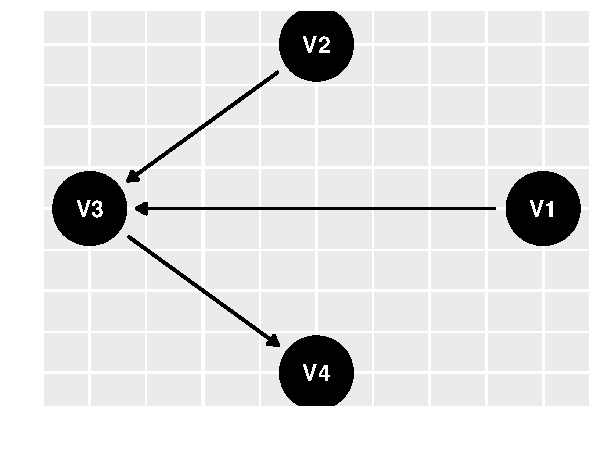
\includegraphics[width=\maxwidth]{./figures/colisor-desc-1} 

}

\caption[Exemplo em que V4 é um descendente de um colisor, V3]{Exemplo em que V4 é um descendente de um colisor, V3.}\label{fig:colisor-desc}
\end{figure}

\end{knitrout}
\end{exercise}

\begin{exercise}
 Prove que se um caminho,
 $C = (C_1, \ldots, C_n)$, está bloqueado
 dado $\V$, então sempre que $C$ é um sub-caminho de $C^*$,
 isto é, $C^* = (A_1, \ldots, A_m, C_1, \ldots, C_n, B_1, \ldots, B_l)$,
 temos que $C^*$ está bloqueado dado $\V$.
\end{exercise}

\begin{exercise}
 Prove que se $\V_1 \perp \V_3 | \V_4$ e
 $\V_2 \perp \V_3 | \V_4$, então
 $\V_1 \cup \V_2 \perp \V_3 | \V_4$.
\end{exercise}

\begin{exercise}
 Prove que se $\V_1 \perp \V_2 | \V_3$, então
 para todo $V \in \sV$, 
 $V \perp \V_1 | \V_3$ ou
 $V \perp \V_2 | \V_3$.
\end{exercise}

\chapter{Intervenções}
\label{cap:intervencao}

% Add: Fórmula do ajuste com score de propensidade
% Add: Demonstração IPW

\section{O modelo de probabilidade para intervenções}

Com base no modelo estrutural causal discutido 
no \cref{cap:dag}, agora estabeleceremos
um significado para o efeito causal
de uma variável em outra.

\begin{knitrout}
\definecolor{shadecolor}{rgb}{0.969, 0.969, 0.969}\color{fgcolor}\begin{figure}

{\centering 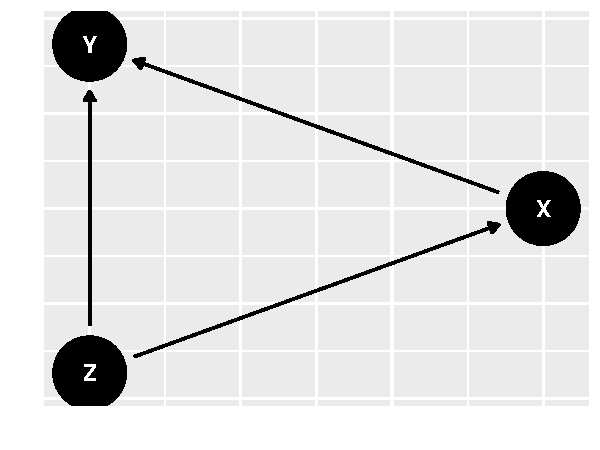
\includegraphics[width=\maxwidth]{./figures/simpson_sexo-1} 

}

\caption[Grafo que representa as relações causais entre Z (Sexo), X (Tratamento), e Y (Cura)]{Grafo que representa as relações causais entre Z (Sexo), X (Tratamento), e Y (Cura).}\label{fig:simpson_sexo}
\end{figure}

\end{knitrout}

Para iniciar esta discussão, considere
as variáveis $Z$ (Sexo), $X$ (Tratamento), 
e $Y$ (Cura), discutidas no \cref{cap:intro}.
Podemos considerar que $Z$ é uma causa
tanto de $X$ quanto de $Y$ e que
$X$ é uma causa de $Y$. Assim,
podemos representar as relações causais 
entre estas variáveis por meio do grafo
na \cref{fig:simpson_sexo}.
Usando este grafo, podemos 
discutir mais a fundo porque 
a probabilidade condicional de cura dado tratamento é
distinta do efeito causal do tratamento na cura.

Quando calculamos a probabilidade condicional
de cura dado o tratamento, estamos perguntando:
``Qual é a probabilidade de que um indivíduo selecionado
  aleatoriamente da população se cure dado que
  \textbf{aprendemos} que recebeu o tratamento?''
Para responder a esta pergunta, propagamos
a informação do tratamento usado em 
todos os caminhos do tratamento para a cura.
Assim, além do efeito direto que o tratamento tem na cura,
o tratamento também está associado ao sexo do paciente,
o que indiretamente traz mais informação sobre a cura deste.
Isto é, neste caso o tratamento traz informação
tanto sobre seus efeitos (cura), 
quanto sobre suas causas (sexo).
Uma outra maneira de verificar estas afirmações é
calculando diretamente $f(y|x)$:
\begin{align}
 \label{eq:prob_causa_1}
 f(y|x)
 &= \sum_s f(z,y|x) \nonumber \\
 &= \sum_s \frac{f(z,y,x)}{f(x)} \nonumber \\
 &= \sum_s \frac{f(z,x)f(y|z,x)}{f(x)} \nonumber \\
 &= \sum_s f(z|x)f(y|z,x)
\end{align}
Notamos na \cref{eq:prob_causa_1} que 
$f(y|x)$ é a média das probabilidades de cura em 
cada sexo, $f(y|z,x)$,
ponderadas pela distribuição do sexo
após aprender o tratamento do indivíduo, $f(z|x)$.

A probabilidade condicional de cura dado tratamento
não corresponde àquilo que entendemos por
efeito causal de tratamento em cura. 
Este efeito é a resposta para a pergunta:
``Qual a probabilidade de que um indivíduo selecionado
  aleatoriamente da população se cure dado que
  \textbf{prescrevemos} a ele o tratamento?''.
Ao contrário da primeira pergunta,
em que apenas \textbf{observamos} a população,
nesta segunda fazemos uma \textbf{intervenção} sobre
o comportamento do indivíduo.
Assim, estamos fazendo uma pergunta sobre 
uma distribuição de probabilidade diferente,
em que estamos agindo sobre a unidade amostral.
Por exemplo, suponha que prescreveríamos o tratamento
a qualquer indivíduo que fosse amostrado.
Neste caso, saber qual tratamento foi aplicado 
não traria qualquer informação sobre o sexo do indivíduo.
Em outras palavras, se chamarmos $f(y|do(x))$ como
a probabilidade de cura dado que fazemos uma intervenção no tratamento,
faria sentido obtermos:
\begin{align}
 \label{eq:prob_causa_2}
 f(y|do(x)) 
 &= \sum_s f(z)f(y|z,x)
\end{align}
Na \cref{eq:prob_causa_2} temos que o efeito causal 
do tratamento na cura é a média ponderada
das probabilidades de cura em cada sexo ponderada
pelas probabilidades de sexo 
de um indivíduo retirado aleatoriamente da população.
Isto é, ao contrário da \cref{eq:prob_causa_1},
a distribuição do sexo do indivíduo não é alterada quando
fazemos uma intervenção sobre o tratamento.

\begin{knitrout}
\definecolor{shadecolor}{rgb}{0.969, 0.969, 0.969}\color{fgcolor}\begin{figure}

{\centering 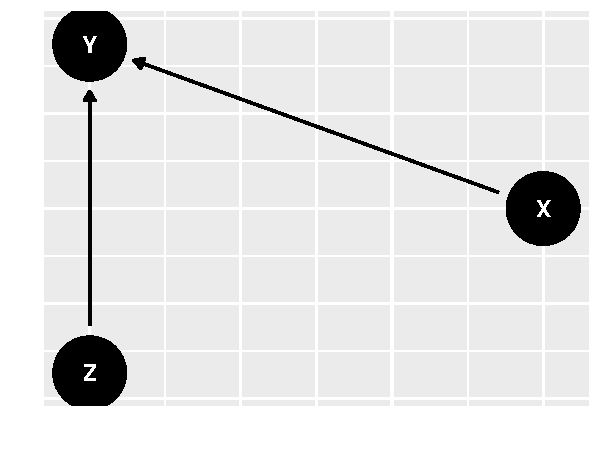
\includegraphics[width=\maxwidth]{./figures/simpson_sexo_inter-1} 

}

\caption[Grafo que representa as relações causais entre S (Sexo), T (Tratamento), e C (Cura) quando há uma intervenção sobre T]{Grafo que representa as relações causais entre S (Sexo), T (Tratamento), e C (Cura) quando há uma intervenção sobre T.}\label{fig:simpson_sexo_inter}
\end{figure}

\end{knitrout}


Com base neste exemplo, podemos generalizar
o que entendemos por intervenção.
Quando fazemos uma intervenção em uma variável, $V_1$,
tomamos uma ação para que $V_1$ assuma um determinado valor.
Assim, as demais variáveis que comumente seriam 
causas de $V_1$ deixam de sê-lo.
Por exemplo, para o caso na \cref{fig:simpson_sexo},
o modelo de intervenção removeria a aresta de
Sexo para Tratamento, resultado na \cref{fig:simpson_sexo_inter}.

Com base nas observações acima, finalmente
podemos definir o modelo de probabilidade sob intervenção:

\begin{definition}
 \label{def:intervencao}
 Seja $\sG = (\sV, \sE)$ um DAG,
 $(\sG,f)$ um SCM (\cref{def:scm}),
 $\V_1 \subseteq \sV$, e 
 $\V_2 = \sV - \V_1$. 
 O modelo de probabilidade obtido após
 uma intervenção em $\V_1$ é dado por:
 \begin{align*}
  f(\V_2|do(\V_1))
  &:= \prod_{V_2 \in \V_2} f(V_2|Pa(V_2))
  &\text{, ou equivalentemente} \\
  f(\V_2|do(\V_1 = \bv_1))
  &:= \left(\prod_{(v_1,V_1) \in (\bv_1,\V_1)} \I(V_1 = v_1)\right)
  \cdot \left(\prod_{V_2 \in \V_2} f(V_2|Pa(V_2))\right)
 \end{align*}
\end{definition}
Para compreender a \cref{def:intervencao}, 
podemos comparar o modelo de intervenção com
o modelo observacional:
\begin{align*}
 f(\V_2|\V_1)
 &\propto f(\V_1,\V_2)
 = \left(\prod_{V_1 \in \V_1}f(V_1|Pa(V_1)\right) \cdot
   \left(\prod_{V_2 \in \V_2}f(V_2|Pa(V_2)\right)
\end{align*}
No modelo observacional, a densidade de $\V_2$ dado $\V_1$ é
proporcional ao produto, para todos os vértices,
da densidade do vértice dadas suas causas.
Ao contrário, no modelo de intervenção supomos que
os vértices em $\V_1$ são pré-fixados e, assim,
não são gerados por suas causas usuais.
Assim, na \cref{def:intervencao},
a densidade de $\V_2$ dada uma intervenção em $\V_1$ é
dada o produto somente nos vértices de $\V_2$
das densidades do vértice dadas suas causas.

Com base na discussão acima, podemos definir
o \textbf{efeito causal} que um conjunto de variáveis, $\X$,
tem em outro conjunto, $\Y$.

\begin{definition}
 \label{def:exp_inter}
 $\E[\Y|do(\X)] := \int \y \cdot f(\y|do(\X)) d\y$.
\end{definition}

\begin{definition}
 \label{def:ace}
 O efeito causal médio, \ACE,\footnote{
 A sigla ACE tem como origem a expressão em inglês,
 \textit{Average Causal Effect}. Optamos por manter a sigla 
 sem tradução para facilitar a comparação com artigos da área.
 Em outros contextos, este termo também é chamado de 
 \textit{Average Treatment Effect} e recebe o acrônimo ATE.}
 de $X \in \Re$ em $Y \in \Re$ é dado por:
 \begin{align*}
  \ACE &=
  \begin{cases}
   \E[Y|do(X=1)] - \E[Y|do(X=0)]
   & \text{, se $X$ é binário}, \\
   \frac{d\E[Y|do(X=x)]}{dx}
   & \text{, se $X$ é contínuo}.
  \end{cases}
 \end{align*}
\end{definition}

Com a \cref{def:ace} podemos finalmente desvendar
o Paradoxo de Simpson discutido no \cref{cap:intro}.
Veremos que o método que desenvolvemos resolve
a questão com simplicidade,
assim trazendo clareza ao Paradoxo.

\begin{example}
 \label{ex:simpson_fim}
 Considere que $(X,Y,Z) \in \Re^3$ são tais que
 $X$ e $Y$ são as indicadores de que, respectivamente, 
 o paciente recebeu o tratamento e se curou. 
 Além disso, suponha que a distribuição conjunta de $(X,Y,Z)$ é
 dada pelas frequências na \cref{tabs:simpson}. Isto é:
 \begin{align*}
  &\P(Z = 1) = \frac{25+55+71+192}{750} \approx 0.46 \\
  &\P(Z = 1|X = 0) = \frac{25+55}{25+55+36+234} \approx 0.23 \\
  &\P(Z = 1|X = 1) = \frac{71+192}{71+192+6+81} \approx 0.75 \\
  &\P(Y = 1|X = 0, Z = 0) = \frac{234}{234+36} \approx 0.87 \\
  &\P(Y = 1|X = 1, Z = 0) = \frac{81}{81+6} \approx 0.93 \\
  &\P(Y = 1|X = 0, Z = 1) = \frac{55}{25+55} \approx 0.69 \\
  &\P(Y = 1|X = 1, Z = 1) = \frac{192}{71+192} \approx 0.73
 \end{align*}
 Agora, veremos que a probabilidade de $Y$ 
 dada uma intervenção em $X$ depende do DAG usado
 no modelo causal estrutural.
 
 Suponha que $Z$ é a indicadora de que 
 o sexo do paciente é masculino.
 Neste caso, utilizarem como 
 grafo causal aquele em \cref{fig:simpson_sexo}.
 Utilizando este grafo, obtemos:
 \begin{align}
  \label{eq:simpson_sexo}
  \P_1(Y=i,Z=j|do(X=k))
  &= \P(Z=j)\P(Y=i|X=k,Z=j) 
  & \text{\cref{def:intervencao}}
 \end{align}
 Assim,
 \begin{align*}
  \P_1(Y=1|do(X=1))
  &= \P_1(Y=1,Z=0|do(X=1)) + \P_1(Y=1,Z=1|do(X=1)) \\
  &= \P(Z=0)\P(Y=1|X=1,Z=0) + \P(Z=1)\P(Y=1|X=1,Z=1)
  & \text{\cref{eq:simpson_sexo}} \\
  &\approx 0.54 \cdot 0.93 + 0.46 \cdot 0.73 \approx 0.84 \\
  \P_1(Y=1|do(X=0))
  &= \P_1(Y=1,Z=0|do(X=0)) + \P_1(Y=1,Z=1|do(X=0)) \\
  &= \P(Z=0)\P(Y=1|X=0,Z=0) + \P(Z=1)\P(Y=1|X=0,Z=1)
  & \text{\cref{eq:simpson_sexo}} \\
  &\approx 0.54 \cdot 0.87 + 0.46 \cdot 0.69 \approx 0.79 \\
 \end{align*}
 Portanto, o efeito causal do tratamento na cura quando
 $Z$ é o sexo do paciente é obtido abaixo:
 \begin{align*}
  \ACE_1 &= \E_1[Y|do(X=1)] - \E_1[Y|do(X=0)] 
  & \text{\cref{def:ace}} \\
  &= \P_1(Y=1|do(X=1)) - \P_1(Y=1|do(X=0)) \approx 0.05
  & \text{\cref{def:exp_inter}}
 \end{align*}
 Como esperado da discussão na \cref{sec:simpson},
 o tratamento tem efeito causal médio positivo, isto é,
 ele aumenta a probabilidade de cura do paciente.
 
\begin{knitrout}
\definecolor{shadecolor}{rgb}{0.969, 0.969, 0.969}\color{fgcolor}\begin{figure}

{\centering 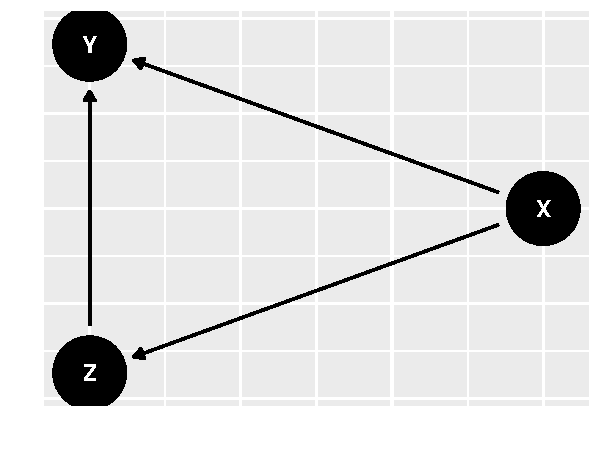
\includegraphics[width=\maxwidth]{./figures/simpson_pressao-1} 

}

\caption[Grafo que representa as relações causais entre Z (Pressão sanguínea elevada), X (Tratamento), e Y (Cura)]{Grafo que representa as relações causais entre Z (Pressão sanguínea elevada), X (Tratamento), e Y (Cura).}\label{fig:simpson_pressao}
\end{figure}

\end{knitrout}
 
 A seguir, consideramos que $Z$ é
 a indicadora de pressão sanguínea elevada do paciente.
 Assim, tomamos o grafo causal como 
 aquele na \cref{fig:simpson_pressao}.
 Utilizando este grafo, obtemos:
 \begin{align}
  \label{eq:simpson_pressao}
  \P_2(Y=i,Z=j|do(X=k))
  &= \P(Z=j|X=k)\P_1(Y=i|X=k,Z=j) 
  & \text{\cref{def:intervencao}}
 \end{align}
 Assim,
 \begin{align*}
  \P_2(Y=1|do(X=1))
  &= \P_2(Y=1,Z=0|do(X=1)) + \P_2(Y=1,Z=1|do(X=1)) \\
  &= \P(Z=0|X=1)\P(Y=1|X=1,Z=0) + \P(Z=1|X=1)\P(Y=1|X=1,Z=1)
  & \text{\cref{eq:simpson_pressao}} \\
  &\approx 0.25 \cdot 0.93 + 0.75 \cdot 0.73 \approx 0.78 \\
  \P_2(Y=1|do(X=0))
  &= \P_2(Y=1,Z=0|do(X=0)) + \P_2(Y=1,Z=1|do(X=0)) \\
  &= \P(Z=0|X=0)\P(Y=1|X=0,Z=0) + \P(Z=1|X=0)\P(Y=1|X=0,Z=1)
  & \text{\cref{eq:simpson_pressao}} \\
  &\approx 0.77 \cdot 0.87 + 0.23 \cdot 0.69 \approx 0.83 \\
 \end{align*}
 Portanto, o efeito causal do tratamento na cura quando
 $Z$ é a pressão sanguínea do paciente é obtido abaixo:
 \begin{align*}
  \ACE_1 &= \E_2[Y|do(X=1)] - \E_2[Y|do(X=0)] 
  & \text{\cref{def:ace}} \\
  &= \P_2(Y=1|do(X=1)) - \P_2(Y=1|do(X=0)) \approx -0.05
  & \text{\cref{def:exp_inter}}
 \end{align*}
 Como esperado da discussão na \cref{sec:simpson},
 o tratamento tem efeito causal médio negativo, isto é,
 ele tem como efeito colateral grave a
 elevação da pressão sanguínea do paciente,
 reduzindo a probabilidade de cura deste.
 
 Comparando as expressões obtidas em $\ACE_1$ e $\ACE_2$,
 verificamos que o grafo causal desempenha papel fundamental
 na determinação do modelo de probabilidade sob intervenção.
 Ademais, o uso do grafo causal adequado em cada situação formaliza
 a discussão qualitativa desenvolvida na \cref{sec:simpson}.
 Não há paradoxo!
\end{example}

Além do efeito causal médio, 
às vezes desejamos determinar 
o efeito causal de $X$ em $Y$ quando
observamos que a unidade amostral
faz parte de determinado estrato da população.
Em outras palavras, desejamos saber 
o efeito causal de $X$ em $Y$ quando observamos que
outras variáveis, $\Z$, assumem um determinado valor.

\begin{definition}
 \label{def:cace}
 O efeito causal médio condicional, \CACE,
 de $X \in \Re$ em $Y \in \Re$ dado $\Z$ é:
 \begin{align*}
  \CACE(\Z) &=
  \begin{cases}
   \E[Y|do(X=1),\Z] - \E[Y|do(X=0),\Z]
   & \text{, se $X$ é binário}, \\
   \frac{d\E[Y|do(X=x),\Z]}{dx}
   & \text{, se $X$ é contínuo}.
  \end{cases}
 \end{align*}
\end{definition}

Uma vez estabelecido o modelo de probabilidade
utilizado quando estudamos intervenções,
agora podemos fazer inferência sobre o efeito causal.
Para realizar tal inferência, 
em geral teremos de abordar duas questões:

\begin{enumerate}
 \item \textbf{Identificação causal}: Temos acesso a dados que 
 são gerados segundo a distribuição observacional.
 Como é possível determinar o efeito causal
 em termos da distribuição observacional?
 
 \item \textbf{Estimação}: Uma vez estabelecida 
 uma ligação entre a distribuição observacional dos dados e
 o efeito causal, como é possível estimá-lo?
\end{enumerate}

Nas próximas seções estudaremos 
algumas estratégias gerais para 
a resolução destas questões.
Consideraremos que desejamos medir
o efeito causal de $X$ em $Y$, 
onde $X, Y \in \sV$.

\subsection{Exercícios}

\begin{exercise}
 Considere que $X_1$ e $X_2$ são variáveis binárias.
 Também considere as seguintes definições:
 \textbf{ACE} := $\P(X_2=1|do(X_1=1))-\P(X_2=1|do(X_1=0))$, e
 \textbf{RD} := $\P(X_2=1|X_1=1)-\P(X_2=1|X_1=0)$.
 Explique em palavras a diferença entre ACE e RD e
 apresente um exemplo em que essa diferença ocorre.
\end{exercise}

\begin{exercise}[{\citet{Glymour2016}[p.32]}]
 $(X_1,X_2,X_3,X_4)$ são 
 variáveis binárias tais que
 $X_{i-1}$ é a única causa imediata de $X_i$.
 Além disso, $\P(X_1=1)=0.5$,
 $\P(X_i=1|X_{i-1}=1)=p_{11}$ e
 $\P(X_i=1|X_{i-1}=0)=p_{01}$.
 Calcule:
 \begin{enumerate}[label=(\alph*)]
  \item $\P(X_1=1,X_2=0,X_3=1,X_4=0)$,
  \item $\P(X_4=1|X_1=1)$, $\P(X_4=1|do(X_1=1)$, 
  \item $\P(X_1=1|X_4=1)$, $\P(X_1=1|do(X_4=1)$, e
  \item $\P(X_3=1|X_1=0,X_4=1)$
 \end{enumerate}
\end{exercise}

\begin{exercise}[{\citet{Glymour2016}[p.29]}]
 Considere que $(U_1, U_2, U_3)$ são independentes e
 tais que $U_i \sim N(0,1)$. Também,
 $X_1 \equiv U_1$,
 $X_2 \equiv 3^{-1}X_1 + U_2$, e
 $X_3 \equiv 2^{-4}X_2 + U_3$.
 Considere que $X_1$ é 
 a causa imediata de $X_2$,
 que por sua vez é a causa imediata de $X_3$.
 Além disso, cada $U_i$ influencia diretamente somente $X_i$.
 \begin{enumerate}[label=(\alph*)]
  \item Desenhe o DAG que representa 
  a estrutura causal indicada no enunciado. 
  \item Calcule $\E[X_2|X_1 = 3]$ e $\E[X_2|do(X_1 = 3)]$.
  \item Calcule $\E[X_3|X_1 = 6]$ e $\E[X_3|do(X_1 = 6)]$.
  \item Calcule $\E[X_1|X_2 = 1]$ e $\E[X_1|do(X_2 = 1)]$.
  \item Calcule $\E[X_2|X_1 = 1, X_3 = 3]$,
  $\E[X_2|X_1 = 1, do(X_3 = 3)]$, e
  $\E[X_2|do(X_1 = 1), X_3 = 3]$.
 \end{enumerate}
\end{exercise}

\section{Controlando confundidores (critério \textit{backdoor})}
\label{sec:backdoor}

Um confundidor é uma causa comum, 
direta ou indireta, de $X$ em $Y$.
Na existência de confundidores,
a regressão de $Y$ em $X$ no modelo observacional, 
$\E[Y|X]$, é diferente desta regressão
no modelo de intervenção, $\E[Y|do(X)]$.
Isto ocorre pois, quando calculamos $\E[Y|X]$,
utilizamos toda a informação em $X$ para prever $Y$.
Esta informação inclui não apenas 
o efeito causal de $X$ em $Y$, como 
também a informação que $X$ traz indiretamente sobre $Y$ 
pelo fato de ambas estarem associados aos seus confundidores.

Para ilustrar este raciocínio, 
podemos revisitar o \cref{ex:simpson_fim}.
uma vez que Sexo (Z) é causa comum do Tratamento (X) e
da Cura (Y), Z é um confundidor.
Quando calculamos $f(y|x)$ (\cref{eq:prob_causa_1}), 
utilizamos não só o efeito direto de $X$ em $Y$, 
expresso em $f(y|x,z)$, como também 
a informação que indireta que $X$ traz sobre $Y$
por meio do confundidor $Z$,
expressa pela combinação de $f(z|x)$ com $f(y|x,z)$.

Esta seção desenvolve uma estratégia para
medir o efeito causal chamada de 
critério \textit{backdoor}, que
consiste em bloquear 
todos os caminhos de informação que passam por confundidores:

\begin{definition}
 \label{def:backdoor}
 Seja $\sG = (\sV, \sE)$ um grafo causal e $X, Y \in \sV$.
 Dizemos que $\Z \subseteq \sV - \{X,Y\}$ satisfaz 
 o critério ``backdoor'' se:
 \begin{itemize}
  \item $X \notin Anc(\Z)$,
  \item Para todo caminho de $X$ em $Y$, 
  $C = (X, C_2, \ldots, C_{n-1}, Y)$ tal que
  $(C_2, X) \in \sE$, $C$ está bloqueado dado $\Z$.
 \end{itemize}
\end{definition}

\begin{example}
 No \cref{ex:simpson_fim} o único caminho de $X$ em $Y$ em que
 o vértice ligado a $X$ é pai de $X$ é $X \leftarrow Z \rightarrow Y$.
 Como $Z$ é um confudidor neste caminho, ele o bloqueia.
 Assim, $Z$ satisfaz o critério backdoor.
\end{example}

\begin{example}
\begin{knitrout}
\definecolor{shadecolor}{rgb}{0.969, 0.969, 0.969}\color{fgcolor}\begin{figure}[t]

{\centering 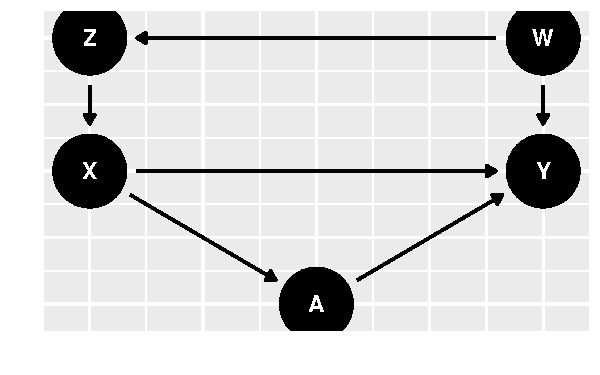
\includegraphics[width=\maxwidth]{./figures/backdoor_ex_1-1} 

}

\caption[Para medir o efeito causal de X em Y, podemos aplicar o critério backdoor]{Para medir o efeito causal de X em Y, podemos aplicar o critério backdoor. Neste grafo o único caminho aplicável ao critério backdoor é (X, Z, W, Y). Neste caminho, $Z$ é uma cadeia e $W$ é um confundidor. Assim, todas as possibilidades dentre Z, W, (Z,W) bloqueiam o caminho e satisfazem o critério backdoor.}\label{fig:backdoor_ex_1}
\end{figure}

\end{knitrout}

 Considere o grafo causal na \cref{fig:backdoor_ex_1}.
 Para aplicar o critério backdoor, devemos identificar
 todos os caminhos de $X$ em $Y$ em que
 o vértice ligado a $X$ é pai de $X$, isto é,
 temos $X \leftarrow$. O único caminho deste tipo é:
 $X \leftarrow Z \leftarrow W \rightarrow Y$.
 Neste caminho, $Z$ é uma cadeia e $W$ é um confudidor.
 Assim, é possível bloquear este caminho condicionando
 em $Z$, em $W$, e em $(Z,W)$.
 Isto é, todos estas combinações 
 satisfazem o critério backdoor.
\end{example}

\begin{example}
\begin{knitrout}
\definecolor{shadecolor}{rgb}{0.969, 0.969, 0.969}\color{fgcolor}\begin{figure}[t]

{\centering 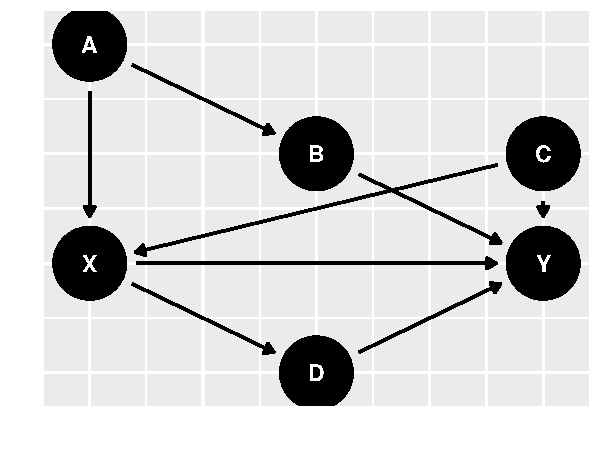
\includegraphics[width=\maxwidth]{./figures/backdoor_ex_2-1} 

}

\caption[Para medir o efeito causal de X em Y, podemos aplicar o critério backdoor]{Para medir o efeito causal de X em Y, podemos aplicar o critério backdoor. Neste grafo existem dois caminhos aplicáveis ao critério backdoor: (X, A, B, Y) e (X, C, Y). No primeiro, A é um confundidor. No segundo caminho, C é um confudidor. Assim, (A,C) bloqueia ambos os caminhos e satisfaz o critério backdoor.}\label{fig:backdoor_ex_2}
\end{figure}

\end{knitrout}

 Considere o grafo causal na \cref{fig:backdoor_ex_2}.
 Para aplicar o critério backdoor,
 encontramos todos os caminhos de $X$ em $Y$ em que
 o vértice ligado a $X$ é pai de $X$. 
 Há dois caminhos deste tipo:
 $X \leftarrow A \rightarrow B \rightarrow Y$ e
 $X \leftarrow C \rightarrow Y$.
 Como $A$ e $C$ são confudidores, respectivamente,
 no primeiro e segundo caminhos, 
 $(A,C)$ bloqueia ambos eles.
 Assim $(A,C)$ satisfaz o critério backdoor.
 Você consegue encontrar outro conjunto de variáveis que
 satisfaz o critério backdoor?
 
 Também é possível identificar 
 os conjuntos de variáveis que satisfazem
 o critério backdoor por meio
 do pacote \textit{dagitty},
 como ilustrado a seguir:
 
\begin{knitrout}
\definecolor{shadecolor}{rgb}{0.969, 0.969, 0.969}\color{fgcolor}\begin{kframe}
\begin{alltt}
\hlkwd{library}\hlstd{(dagitty)}
\hlcom{# Especificar o grafo}
\hlstd{grafo} \hlkwb{<-} \hlkwd{dagitty}\hlstd{(}\hlstr{"dag\{
    X[e] Y[o]
    A -> \{ X B \}; B -> \{ Y \}; C -> \{ X Y \};
    X -> \{ D Y \}; D -> Y \}"}\hlstd{)}

\hlkwd{adjustmentSets}\hlstd{(grafo,} \hlkwc{type} \hlstd{=} \hlstr{"all"}\hlstd{)}
\end{alltt}
\begin{verbatim}
## { A, C }
## { B, C }
## { A, B, C }
\end{verbatim}
\end{kframe}
\end{knitrout}
\end{example}

O critério backdoor generaliza duas condições especiais que
são muito utilizadas.
Em uma primeira condição, 
o valor de $X$ é gerado integralmente por
um aleatorizador, independente de todas as demais variáveis.
Esta ideia é captada pela 
\cref{def:aleatorizacao}, abaixo:

\begin{definition}
 \label{def:aleatorizacao}
 Dizemos que $X$ é um experimento aleatorizado simples 
 se $X$ é ancestral.
\end{definition}

Em um experimento aleatorizado simples não há confundidores.
Assim, $\emptyset$ satisfaz o critério backdoor:

\begin{lemma}
 \label{lemma:backdoor_random}
 Se $X$ é um experimento aleatorizado simples, então
 $\emptyset$ satisfaz o critério backdoor.
\end{lemma}

Veremos que em um experimento aleatorizado simples a
distribuição intervencional é igual 
à distribuição observacional.
Assim, $\E[Y|do(X)] = \E[Y|X]$ e
a inferência causal é reduzida 
à inferência comumente usadas para
a distribuição observacional.

Além disso, o conjunto de todos os pais de $X$
também satisfaz o critério backdoor:

\begin{lemma}
 \label{lemma:backdoor_pais}
 $\Z = Pa(X)$ satisfaz o critério backdoor para
 medir o efeito causal de $X$ em $Y$.
\end{lemma}

A seguir, veremos como o critério backdoor permite
a identificação causal, isto é,
uma equivalência entre quantidades de interesse
obtidas pelo modelo de intervenção e
quantidades obtidas pelo modelo observacional.

\subsection{Identificação causal usando o critério backdoor}

A seguir, o \cref{thm:backdoor} mostra que,
se $\Z$ satisfaz o critério backdoor, então
é possível ligar algumas 
distribuições sob intervenção em $X$ a
distribuições observacionais:

\begin{theorem}
 \label{thm:backdoor}
 Se $\Z$ satisfaz 
 o critério backdoor para medir
 o efeito causal de $X$ em $Y$, então
 \begin{align*}
  f(\z|do(x)) 
  &= f(\z), \text{ e } \\
  f(y|do(x), \z) 
  &= f(y|x, \z).
 \end{align*}
\end{theorem}

O \cref{thm:backdoor} mostra que,
se $\Z$ satisfaz o critério backdoor, então
distribuição de $\Z$ quando
aplicamos uma intervenção em $X$ é igual
à distribuição marginal de $\Z$.
Além disso, a distribuição condicional de
$Y$ dado $\Z$ quando aplicamos uma intervenção em $X$ é igual 
à distribuição de $Y$ dado $X$ e $Z$.
Assim, o \cref{thm:backdoor} relaciona
distribuições que não geraram os dados a 
distribuições que os geraram.
Com base neste resultado, é possível determinar
$f(y|do(x))$ a partir de $f(y,x,\z)$:

\begin{corollary}
 \label{cor:backdoor}
 Se $\Z$ satisfaz 
 o critério backdoor para medir
 o efeito causal de $X$ em $Y$, então
 \begin{align*}
  f(y|do(x)) &=
  \int f(y|x,\z)f(\z)d\z.
 \end{align*}
\end{corollary}

Para compreender intuitivamente o \cref{cor:backdoor},
podemos retornar ao \cref{ex:simpson_fim}.
Considere o caso em que $X, Y, Z$ são as indicadoras de que,
respectivamente, o paciente foi submetido ao tratamento,
se curou e, é de sexo masculino.
Similarmente ao \cref{thm:backdoor},
vimos em \cref{ex:simpson_fim} que $f(y|do(x))$ é
a média de $f(y|x,z)$ ponderada por $f(z)$.
Nesta ponderação, utilizamos $f(z)$ 
ao invés de $f(z|x)$ pois $Z$ é um confundidor e,
assim, no modelo intervencional não propagamos
a informação em $X$ por esta variável.
A mesma lógica se aplica 
às variáveis que satisfazem o critério backdoor.

Para calcular quantidades 
como o $\ACE$ (\cref{def:ace}), 
utilizamos $\E[Y|do(X)]$.
Por meio do \cref{thm:backdoor},
é possível obter equivalências entre
$\E[Y|do(X)]$ e esperanças obtidas
no modelo observacional.
Estas equivalências são descritas
nos \cref{thm:backdoor_ajuste,thm:backdoor_ipw}.

\begin{theorem}
 \label{thm:backdoor_ajuste}
 Se $\Z$ satisfaz 
 o critério backdoor para medir
 o efeito causal de $X$ em $Y$, então
 \begin{align*}
  \E[g(Y)|do(X=x),\Z]
  &= \E[g(Y)|X=x,\Z], \text{ e } \\
  \E[g(Y)|do(X=x)] 
  &= \E[\E[g(Y)|X=x,\Z]]
 \end{align*}
\end{theorem}

\begin{theorem}
 \label{thm:backdoor_ipw}
 Se $\Z$ satisfaz 
 o critério backdoor para medir
 o efeito causal de $X$ em $Y$ e
 $X$ é discreto, então
 \begin{align*}
  \E[g(Y)|do(X=x),\Z] 
  &= \frac{\E[g(Y)\I(X=x)|\Z]}{f(x|\Z)}, \text{ e } \\
  \E[g(Y)|do(X=x)]
  &= \E\left[\frac{g(Y)\I(X=x)}{f(x|\Z)}\right]
 \end{align*}
\end{theorem}

A seguir, veremos como os
\cref{thm:backdoor_ajuste,thm:backdoor_ipw} podem
ser usados para estimar o efeito causal.
Para provar resultados sobre os estimadores obtidos,
a seguinte definição será útil

\begin{definition}
 \label{def:perm}
 Seja $\hat{g}$ um estimador treinado com
 os dados $(\sV_1,\ldots,\sV_n)$.
 Dizemos que $\hat{g}$ é 
 invariante a permutações se
 o estimador não depende da ordem dos dados.
 Isto é, para qualquer permutações dos índices,
 $\pi: \{1,\ldots,n\} \rightarrow \{1,\ldots,n\}$,
 $\hat{g}(\sV_1,\ldots,\sV_n) \equiv 
 \hat{g}(\sV_{\pi(1)},\ldots,\sV_{\pi(n)})$
\end{definition}

\begin{example}
 \label{ex:perm}
 A média amostral é invariante a permutações pois,
 para qualquer permutação $\pi$,
 \begin{align*}
  \frac{\sum_{i=1}^n X_i}{n} 
  = \frac{\sum_{i=1}^n X_{\pi(i)}}{n}.
 \end{align*} 
\end{example}

\subsection{Estimação usando o critério backdoor}
\label{sec:backdoor_est}

\subsubsection{Fórmula do ajuste}

O \cref{thm:backdoor_ajuste} determina que, 
se $\Z$ satisfaz o critério backdoor, então
$\E[Y|do(X),\Z] = \E[Y|X,\Z]$.
Como $\mu(X,Z) := \E[Y|X,\Z]$ é 
a função de regressão de $Y$ em $X$ e $Z$,
podemos estimar $\mu$ utilizando 
quaisquer métodos de estimação para regressão.
Por exemplo, se $Y$ é contínua,
possíveis métodos são:
regressão linear, Nadaraya-Watson, 
floresta aleatória de regressão, redes neurais, \ldots
Por outro lado, se $Y$ é discreta,
então a função de regressão é estimada por
métodos de classificação como:
regressão logística, k-NN, 
floresta aleatória de classificação,
redes neurais, \ldots
Para qualquer opção escolhida,
denotamos o estimador de $\mu$ por $\hmu$.

Utilizando $\hmu$, podemos estimar
$\CACE(\Z)$ diretamente.
Para tal, note que $\CACE(\Z)$ é
função de $\E[Y|do(X),\Z]$.
Como o \cref{thm:backdoor_ajuste} garante que
$\E[Y|do(X=x),\Z] = \mu(x,\Z)$,
podemos definir o estimador
$\hdoyz := \hmu(x,\Z)$.

O \cref{thm:backdoor_ajuste} também 
orienta a estimação do $\ACE$. 
Similarmente ao caso anterior,
o $\ACE$ é função de $\E[Y|do(X)]$.
Pelo \cref{thm:backdoor_ajuste},
$\E[Y|do(X=x)] = \E[\mu(x,\Z)]$.
Assim, se $\hmu \approx \mu$,
$\E[Y|do(X=x)] \approx \E[\hmu(x,\Z)]$.
Como $\E[\hmu(x,\Z)]$ é simplesmente 
uma média populacional,
podemos estimá-la com base
na média amostral:
\begin{align*}
 \hdoy := \frac{\sum_{i=1}^n \hmu(x,\Z_i)}{n} \approx \E[\hmu(x,\Z)]
\end{align*}

\begin{definition}
 \label{def:ajuste}
 Considere que $\Z$ satisfaz o critério backdoor para
 medir o efeito causal de $X$ em $Y$ e
 $\hmu(x,\z)$ é uma estimativa 
 da regressão $\E[Y|X=x,\Z=\z]$.
 Os estimadores de 
 $\E[Y|do(X=x),\Z]$ e
 $\E[Y|do(X=x)]$ pela
 fórmula do ajuste são:
\begin{align*}
 \hdoyz &:= \hmu(x,\Z) \\
 \hdoy &:= \frac{\sum_{i=1}^n \hmu(x,\Z_i)}{n}
\end{align*}
\end{definition}

A seguir mostraremos que,
se $\hmu$ converge para $\mu$, então
$\hdoy$ converge para $\E[Y|do(X=x)]$.
Em outras palavras, é possível utilizar
$\hdoy$ para estimar o efeito causal de $X$ em $Y$
por meio de expressões como o $\ACE$.

\begin{theorem}
 \label{thm:conv_ajuste}
 Seja $\mu(X,\Z) := \E[Y|X,\Z]$.
 Se $\Z$ satisfaz o critério backdoor para
 medir o efeito causal de $X$ em $Y$,
 $\E[|\mu(x,\Z_1)|] < \infty$,
 $\E[|\hmu(x,\Z_1)-\mu(x,\Z_1)|] = o(1)$, 
 e $\hmu$ é invariante a permutações (\cref{def:perm}), então
 $\hdoy \convp \E[Y|do(X=x)]$.
\end{theorem}

A seguir, utilizamos dados simulados para
ilustrar a implementação da fórmula do ajuste.

\begin{example}
 \label{ex:backdoor_est_ajuste}
\begin{knitrout}
\definecolor{shadecolor}{rgb}{0.969, 0.969, 0.969}\color{fgcolor}\begin{figure}[t]

{\centering 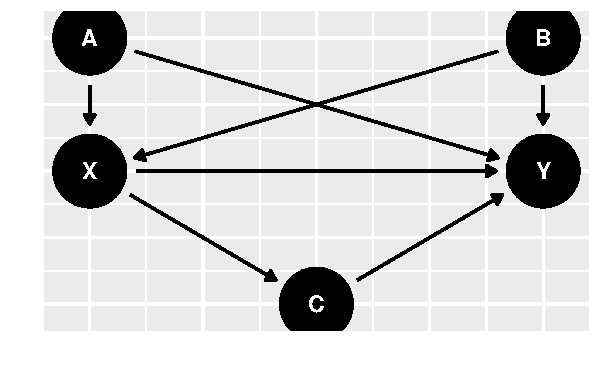
\includegraphics[width=\maxwidth]{./figures/backdoor_est_ex-1} 

}

\caption[DAG usado como exemplo para estimar efeito de X em Y]{DAG usado como exemplo para estimar efeito de X em Y.}\label{fig:backdoor_est_ex}
\end{figure}

\end{knitrout}

Considere que o grafo causal é
dado pela \cref{fig:backdoor_est_ex}.
Vamos supor que os dados são gerados da seguinte forma:
$\sigma^2 = 0.01$,
$A \sim N(0, \sigma^2)$, 
$B \sim N(0, \sigma^2)$,
$\epsilon \sim Bernoulli(0.95)$
$X \equiv \I(A + B > 0)\epsilon + \I(A + B < 0)(1-\epsilon)$,
$C \sim N(X, \sigma^2)$, e
$Y \sim N(A + B + C + X, \sigma^2)$:

\begin{knitrout}
\definecolor{shadecolor}{rgb}{0.969, 0.969, 0.969}\color{fgcolor}\begin{kframe}
\begin{alltt}
\hlcom{# Especificar o grafo}
\hlstd{grafo} \hlkwb{<-} \hlstd{dagitty}\hlopt{::}\hlkwd{dagitty}\hlstd{(}\hlstr{"dag \{
    X[e] Y[o]
    \{A B\} -> \{ X Y \}; X -> \{C Y\}; C -> Y \}"}\hlstd{)}

\hlcom{# Simular os dados}
\hlstd{n} \hlkwb{<-} \hlnum{10}\hlopt{^}\hlnum{5}
\hlstd{sd} \hlkwb{=} \hlnum{0.1}
\hlstd{A} \hlkwb{<-} \hlkwd{rnorm}\hlstd{(n,} \hlnum{0}\hlstd{, sd)}
\hlstd{B} \hlkwb{<-} \hlkwd{rnorm}\hlstd{(n,} \hlnum{0}\hlstd{, sd)}
\hlstd{eps} \hlkwb{<-} \hlkwd{rbinom}\hlstd{(n,} \hlnum{1}\hlstd{,} \hlnum{0.8}\hlstd{)}
\hlstd{X} \hlkwb{<-} \hlkwd{as.numeric}\hlstd{(eps}\hlopt{*}\hlstd{((A} \hlopt{+} \hlstd{B)} \hlopt{>} \hlnum{0}\hlstd{)} \hlopt{+}
                  \hlstd{(}\hlnum{1}\hlopt{-}\hlstd{eps)}\hlopt{*}\hlstd{((A} \hlopt{+} \hlstd{B)} \hlopt{<=} \hlnum{0}\hlstd{))}
\hlstd{C} \hlkwb{<-} \hlkwd{rnorm}\hlstd{(n, X, sd)}
\hlstd{Y} \hlkwb{<-} \hlkwd{rnorm}\hlstd{(n, A} \hlopt{+} \hlstd{B} \hlopt{+} \hlstd{C} \hlopt{+} \hlstd{X, sd)}
\hlstd{data} \hlkwb{<-} \hlstd{dplyr}\hlopt{::}\hlkwd{tibble}\hlstd{(A, B, C, X, Y)}
\end{alltt}
\end{kframe}
\end{knitrout}

Estimaremos o efeito causal pela
fórmula do ajuste (\cref{def:ajuste}).
Iniciaremos a análise utilizando $\hmu$ como
sendo uma regressão linear simples:

\begin{knitrout}
\definecolor{shadecolor}{rgb}{0.969, 0.969, 0.969}\color{fgcolor}\begin{kframe}
\begin{alltt}
\hlcom{# Sejam Z variáveis que satisfazem o critério backdoor para}
\hlcom{# estimar o efeito causal de causa em efeito em grafo.}
\hlcom{# Retorna uma fórmula do tipo Y ~ X + Z_1 + ... + Z_d}
\hlstd{fm_ajuste} \hlkwb{<-} \hlkwa{function}\hlstd{(}\hlkwc{grafo}\hlstd{,} \hlkwc{causa}\hlstd{,} \hlkwc{efeito}\hlstd{)}
\hlstd{\{}
  \hlstd{var_backdoor} \hlkwb{<-} \hlstd{dagitty}\hlopt{::}\hlkwd{adjustmentSets}\hlstd{(grafo)[[}\hlnum{1}\hlstd{]]}
  \hlstd{regressores} \hlkwb{=} \hlkwd{c}\hlstd{(causa, var_backdoor)}
  \hlstd{fm} \hlkwb{=} \hlkwd{paste}\hlstd{(regressores,} \hlkwc{collapse} \hlstd{=} \hlstr{"+"}\hlstd{)}
  \hlstd{fm} \hlkwb{=} \hlkwd{paste}\hlstd{(}\hlkwd{c}\hlstd{(efeito, fm),} \hlkwc{collapse} \hlstd{=} \hlstr{"~"}\hlstd{)}
  \hlkwd{as.formula}\hlstd{(fm)}
\hlstd{\}}

\hlcom{# Estima E[Efeito|do(causa = x)] pela }
\hlcom{# formula do ajuste usando mu_chapeu como regressao }
\hlstd{est_do_x_lm} \hlkwb{<-} \hlkwa{function}\hlstd{(}\hlkwc{data}\hlstd{,} \hlkwc{mu_chapeu}\hlstd{,} \hlkwc{causa}\hlstd{,} \hlkwc{x}\hlstd{)}
\hlstd{\{}
  \hlstd{data} \hlopt
    \hlstd{dplyr}\hlopt{::}\hlkwd{mutate}\hlstd{(\{\{causa\}\}} \hlkwb{:=} \hlstd{x)} \hlopt
    \hlkwd{predict}\hlstd{(mu_chapeu,} \hlkwc{newdata} \hlstd{= .)} \hlopt
    \hlkwd{mean}\hlstd{()}
\hlstd{\}}

\hlcom{# Estimação do ACE com regressão linear simples}
\hlstd{fm} \hlkwb{<-} \hlkwd{fm_ajuste}\hlstd{(grafo,} \hlstr{"X"}\hlstd{,} \hlstr{"Y"}\hlstd{)}
\hlstd{mu_chapeu_lm} \hlkwb{<-} \hlkwd{lm}\hlstd{(fm,} \hlkwc{data} \hlstd{= data)}
\hlstd{ace_ajuste_lm} \hlkwb{=} \hlkwd{est_do_x_lm}\hlstd{(data, mu_chapeu_lm,} \hlstr{"X"}\hlstd{,} \hlnum{1}\hlstd{)} \hlopt{-}
  \hlkwd{est_do_x_lm}\hlstd{(data, mu_chapeu_lm,} \hlstr{"X"}\hlstd{,} \hlnum{0}\hlstd{)}
\hlkwd{round}\hlstd{(ace_ajuste_lm)}
\end{alltt}
\begin{verbatim}
## [1] 2
\end{verbatim}
\end{kframe}
\end{knitrout}

Em alguns casos, não é razoável supor que 
$\E[Y|X,\Z]$ é linear. Nestas situações,
é fácil adaptar o código anterior para
algum método não-paramétrico arbitrário.
Exibimos uma implementação usando XGBoost 
\citep{Chen2023}:

\begin{knitrout}
\definecolor{shadecolor}{rgb}{0.969, 0.969, 0.969}\color{fgcolor}\begin{kframe}
\begin{alltt}
\hlkwd{library}\hlstd{(xgboost)}
\hlstd{var_backdoor} \hlkwb{<-} \hlstd{dagitty}\hlopt{::}\hlkwd{adjustmentSets}\hlstd{(grafo,} \hlstr{"X"}\hlstd{,} \hlstr{"Y"}\hlstd{)[[}\hlnum{1}\hlstd{]]}
\hlstd{mu_chapeu} \hlkwb{<-} \hlkwd{xgboost}\hlstd{(}
  \hlkwc{data} \hlstd{= data} \hlopt
    \hlstd{dplyr}\hlopt{::}\hlkwd{select}\hlstd{(}\hlkwd{all_of}\hlstd{(}\hlkwd{c}\hlstd{(var_backdoor,} \hlstr{"X"}\hlstd{)))} \hlopt
    \hlkwd{as.matrix}\hlstd{(),}
  \hlkwc{label} \hlstd{= data} \hlopt
    \hlstd{dplyr}\hlopt{::}\hlkwd{select}\hlstd{(Y)} \hlopt
    \hlkwd{as.matrix}\hlstd{(),}
  \hlkwc{nrounds} \hlstd{=} \hlnum{100}\hlstd{,}
  \hlkwc{objective} \hlstd{=} \hlstr{"reg:squarederror"}\hlstd{,}
  \hlkwc{early_stopping_rounds} \hlstd{=} \hlnum{3}\hlstd{,}
  \hlkwc{max_depth} \hlstd{=} \hlnum{2}\hlstd{,}
  \hlkwc{eta} \hlstd{=} \hlnum{.25}\hlstd{,}
  \hlkwc{verbose} \hlstd{=} \hlnum{FALSE}
\hlstd{)}

\hlstd{est_do_x_xgb} \hlkwb{<-} \hlkwa{function}\hlstd{(}\hlkwc{data}\hlstd{,} \hlkwc{mu_chapeu}\hlstd{,} \hlkwc{causa}\hlstd{,} \hlkwc{x}\hlstd{)}
\hlstd{\{}
  \hlstd{data} \hlopt
    \hlstd{dplyr}\hlopt{::}\hlkwd{mutate}\hlstd{(\{\{causa\}\}} \hlkwb{:=} \hlstd{x)} \hlopt
    \hlstd{dplyr}\hlopt{::}\hlkwd{select}\hlstd{(}\hlkwd{c}\hlstd{(var_backdoor, causa))} \hlopt
    \hlkwd{as.matrix}\hlstd{()} \hlopt
    \hlkwd{predict}\hlstd{(mu_chapeu,} \hlkwc{newdata} \hlstd{= .)} \hlopt
    \hlkwd{mean}\hlstd{()}
\hlstd{\}}

\hlstd{ace_est_xgb} \hlkwb{=} \hlkwd{est_do_x_xgb}\hlstd{(data, mu_chapeu,} \hlstr{"X"}\hlstd{,} \hlnum{1}\hlstd{)} \hlopt{-}
  \hlkwd{est_do_x_xgb}\hlstd{(data, mu_chapeu,} \hlstr{"X"}\hlstd{,} \hlnum{0}\hlstd{)}
\hlkwd{round}\hlstd{(ace_est_xgb,} \hlnum{2}\hlstd{)}
\end{alltt}
\begin{verbatim}
## [1] 2
\end{verbatim}
\end{kframe}
\end{knitrout}

 Como o modelo linear era adequado para $\E[Y|X,\Z]$,
 não vemos diferença entre a estimativa obtida
 pela regressão linear simples e pelo XGBoost.
 Mas será que as estimativas estão adequadas?
 Como simulamos os dados,
 é possível calcular diretamente $\E[Y|do(X=x)]$:
 \begin{align}
  \label{eq:ex_backdoor_1}
  \E[Y|do(X=x)]
  &= \E[\E[Y|X=x, A, B]]
  & \text{\cref{thm:backdoor_ajuste}} \nonumber \\
  &= \E[\E[\E[Y|X=x, A, B, C]|X=x, A, B]]
  & \text{Lei da esperança total} \nonumber \\
  &= \E[\E[A+B+C+X|X=x, A, B]]
  & Y \sim N(A+B+C+X, \sigma^2) \nonumber \\
  &= \E[A + B + 2x]
  & C \sim N(X, \sigma^2) \nonumber \\
  &= 2x
  & \E[A] = \E[B] = 0
 \end{align}
 Uma vez calculado $\E[Y|do(X=x)]$,
 podemos obter o $\ACE$:
 \begin{align*}
  \ACE
  &= \E[Y|do(X=1)] - \E[Y|do(X=0)] \\
  &= 2 \cdot 1 - 2 \cdot 0 = 2
  & \text{\cref{eq:ex_backdoor_1}}
 \end{align*}
 Portanto, as estimativas do $\ACE$ obtidas 
 pela regressão linear e pelo xgboost 
 estão adequadas.
\end{example}

\subsubsection{Ponderação pelo inverso do escore de propensidade (IPW)}

Uma outra forma de estimar 
$\E[Y|do(X=x)]$ e $\E[Y|do(X=x),\Z]$ é
motivada pelo \cref{thm:backdoor_ipw}.
Este resultado determina que, 
se $\Z$ satisfaz o critério backdoor, então
\begin{align*}
 \E[Y|do(X=x),\Z] 
 &= \frac{\E\left[Y \I(X=x)|\Z\right]}{f(x|\Z)}.
\end{align*}
Na segunda expressão, $\E[Y \I(X=x)|\Z]$ é 
a regressão de $Y\I(X=x)$ em $\Z$.
Assim, esta quantidade pode ser estimada por
um método de regressão arbitrário, que
denotaremos por $\widehat{\E}[Y \I(X=x)|\Z]$.
Também $f(x|\z)$ é 
usualmente chamado de \textit{escore de propensidade}.
Este escore captura a forma como 
os confundidores atuam sobre $X$
nos dados observacionais.
Como $f$ em geral é desconhecido,
$f(x|\z)$ também o é.
Contudo, quando $X$ é discreto,
podemos estimar $f(x|\z)$ utilizando
algum algoritmo arbitrário de classificação.
Denotaremos esta estimativa por $\hf(x|\z)$.
Se a estimativa for boa, temos
\begin{align*}
 \E[Y|do(X=x),\Z]
 &= \frac{\widehat{\E}[Y \I(X=x)|\Z]}{f(x|\Z)}
 \approx \frac{\widehat{\E}[Y \I(X=x)|\Z]}{\hf(x|\z)}.
\end{align*}

O \cref{thm:backdoor_ipw} também orienta
a estimação de $\E[Y|do(X=x)]$.
Se $\Z$ satisfaz o critério backdoor, então
\begin{align*}
 \E[Y|do(X=x)]
 &= \E\left[\frac{Y \I(X=x)}{f(x|\Z)}\right]
\end{align*}
Como nesta expressão a esperança é
uma média populacional,
ela pode ser aproximada pela média amostral
\begin{align*}
 \E\left[\frac{Y \I(X=x)}{f(x|\Z)}\right]
 &\approx n^{-1} \sum_{i=1}^n \frac{Y_i \I(X_i=x)}{\hf(x|\Z_i)}.
\end{align*}

Combinando estas aproximações, obtemos:
\begin{definition}
 \label{def:ipw}
 Considere que $\Z$ satisfaz o critério backdoor para
 medir o efeito causal de $X$ em $Y$ e
 $\hf(x|\z)$ é uma estimativa de $f(x|\z)$.
 Os estimadores de $\E[Y|do(X=x),\Z]$ e $\E[Y|do(X=x)]$ 
 por IPW são:
\begin{align*}
 \hdoyzb &:= \frac{\widehat{\E}[Y \I(X=x)|\Z]}{\hf(x|\z)} \\
 \hdoyb &:= n^{-1} \sum_{i=1}^n \frac{Y_i \I(X_i=x)}{\hf(x|\Z_i)}.
\end{align*}
\end{definition}

Se $\hf$ converge para $f$, então sob 
condições relativamente pouco restritivas
$\hdoyb$ converge para $\E[Y|do(X=x)]$.

\begin{theorem}
 \label{thm:conv_ipw}
 Se $\hf$ é invariante a permutações (\cref{def:perm}),
 $\E[|\hf(x|\Z_1)-f(x|\Z_1)|] = o(1)$, e
 existe $M > 0$ tal que
 $\sup_\z \E[|Y| \I(X=x)|\Z=\z] < M$, e
 existe $\delta > 0$ tal que
 $\inf_z \min\{f(x|\Z_1), \hf(x|\Z_1)\} > \delta$, então
 $\hdoyb \convp \E[Y|do(X=x)]$.
\end{theorem}

A seguir, utilizamos novamente dados simulados para
ilustrar a implementação de IPW:

\begin{example}
\label{ex:backdoor_est_ipw}
Considere que o grafo causal e
o modelo de geração dos dados são 
idênticos àqueles do \cref{ex:backdoor_est_ajuste}.
Iniciaremos a análise utilizando 
regressão logística para estimar $\hf$.
 
\begin{knitrout}
\definecolor{shadecolor}{rgb}{0.969, 0.969, 0.969}\color{fgcolor}\begin{kframe}
\begin{alltt}
\hlcom{# Sejam Z variáveis que satisfazem o critério backdoor para}
\hlcom{# estimar o efeito causal de causa em efeito em grafo.}
\hlcom{# Retorna uma fórmula do tipo X ~ Z_1 + ... + Z_d}
\hlstd{fm_ipw} \hlkwb{<-} \hlkwa{function}\hlstd{(}\hlkwc{grafo}\hlstd{,} \hlkwc{causa}\hlstd{,} \hlkwc{efeito}\hlstd{)}
\hlstd{\{}
 \hlstd{var_backdoor} \hlkwb{<-} \hlstd{dagitty}\hlopt{::}\hlkwd{adjustmentSets}\hlstd{(grafo)[[}\hlnum{1}\hlstd{]]}
 \hlstd{fm} \hlkwb{=} \hlkwd{paste}\hlstd{(var_backdoor,} \hlkwc{collapse} \hlstd{=} \hlstr{"+"}\hlstd{)}
 \hlstd{fm} \hlkwb{=} \hlkwd{paste}\hlstd{(}\hlkwd{c}\hlstd{(causa, fm),} \hlkwc{collapse} \hlstd{=} \hlstr{"~"}\hlstd{)}
 \hlkwd{as.formula}\hlstd{(fm)}
\hlstd{\}}

\hlcom{# Estimação do ACE por IPW onde}
\hlcom{# Supomos X binário e}
\hlcom{# f_1 é o vetor P(X_i=1|Z_i)}
\hlstd{ACE_ipw} \hlkwb{<-} \hlkwa{function}\hlstd{(}\hlkwc{data}\hlstd{,} \hlkwc{causa}\hlstd{,} \hlkwc{efeito}\hlstd{,} \hlkwc{f_1}\hlstd{)}
\hlstd{\{}
 \hlstd{data} \hlopt
 \hlkwd{mutate}\hlstd{(}\hlkwc{f_1} \hlstd{= f_1,}
        \hlkwc{est_1} \hlstd{= \{\{efeito\}\}}\hlopt{*}\hlstd{(\{\{causa\}\}}\hlopt{==}\hlnum{1}\hlstd{)}\hlopt{/}\hlstd{f_1,}
        \hlkwc{est_0} \hlstd{= \{\{efeito\}\}}\hlopt{*}\hlstd{(\{\{causa\}\}}\hlopt{==}\hlnum{0}\hlstd{)}\hlopt{/}\hlstd{(}\hlnum{1}\hlopt{-}\hlstd{f_1)}
 \hlstd{)} \hlopt
 \hlkwd{summarise}\hlstd{(}\hlkwc{do_1} \hlstd{=} \hlkwd{mean}\hlstd{(est_1),}
           \hlkwc{do_0} \hlstd{=} \hlkwd{mean}\hlstd{(est_0))} \hlopt
 \hlkwd{mutate}\hlstd{(}\hlkwc{ACE} \hlstd{= do_1} \hlopt{-} \hlstd{do_0)} \hlopt
 \hlstd{dplyr}\hlopt{::}\hlkwd{select}\hlstd{(ACE)}
\hlstd{\}}

\hlstd{fm} \hlkwb{<-} \hlkwd{fm_ipw}\hlstd{(grafo,} \hlstr{"X"}\hlstd{,} \hlstr{"Y"}\hlstd{)}
\hlstd{f_chapeu} \hlkwb{<-} \hlkwd{glm}\hlstd{(fm,} \hlkwc{family} \hlstd{=} \hlstr{"binomial"}\hlstd{,} \hlkwc{data} \hlstd{= data)}
\hlstd{f_1_lm} \hlkwb{<-} \hlkwd{predict}\hlstd{(f_chapeu,} \hlkwc{type} \hlstd{=} \hlstr{"response"}\hlstd{)}
\hlstd{ace_ipw_lm} \hlkwb{<-} \hlstd{data} \hlopt \hlkwd{ACE_ipw}\hlstd{(X, Y, f_1_lm)} \hlopt \hlkwd{as.numeric}\hlstd{()}
\hlstd{ace_ipw_lm} \hlopt \hlkwd{round}\hlstd{(}\hlnum{2}\hlstd{)}
\end{alltt}
\begin{verbatim}
## [1] 2.09
\end{verbatim}
\end{kframe}
\end{knitrout}

Também é fácil adaptar o código acima para
estimar $\ACE$ por IPW utilizando
algum método não-paramétrico para estimar $\hf$.
Abaixo há um exemplo utilizando o XGBoost:

\begin{knitrout}
\definecolor{shadecolor}{rgb}{0.969, 0.969, 0.969}\color{fgcolor}\begin{kframe}
\begin{alltt}
\hlstd{var_backdoor} \hlkwb{<-} \hlstd{dagitty}\hlopt{::}\hlkwd{adjustmentSets}\hlstd{(grafo)[[}\hlnum{1}\hlstd{]]}
\hlstd{f_chapeu} \hlkwb{<-} \hlkwd{xgboost}\hlstd{(}
 \hlkwc{data} \hlstd{= data} \hlopt
   \hlstd{dplyr}\hlopt{::}\hlkwd{select}\hlstd{(}\hlkwd{all_of}\hlstd{(var_backdoor))} \hlopt
   \hlkwd{as.matrix}\hlstd{(),}
 \hlkwc{label} \hlstd{= data} \hlopt
   \hlstd{dplyr}\hlopt{::}\hlkwd{select}\hlstd{(X)} \hlopt
   \hlkwd{as.matrix}\hlstd{(),}
 \hlkwc{nrounds} \hlstd{=} \hlnum{100}\hlstd{,}
 \hlkwc{objective} \hlstd{=} \hlstr{"binary:logistic"}\hlstd{,}
 \hlkwc{early_stopping_rounds} \hlstd{=} \hlnum{3}\hlstd{,}
 \hlkwc{max_depth} \hlstd{=} \hlnum{2}\hlstd{,}
 \hlkwc{eta} \hlstd{=} \hlnum{.25}\hlstd{,}
 \hlkwc{verbose} \hlstd{=} \hlnum{FALSE}
\hlstd{)}

\hlstd{covs} \hlkwb{<-} \hlstd{data} \hlopt \hlstd{dplyr}\hlopt{::}\hlkwd{select}\hlstd{(}\hlkwd{all_of}\hlstd{(var_backdoor))} \hlopt \hlkwd{as.matrix}\hlstd{()}
\hlstd{f_1} \hlkwb{<-} \hlkwd{predict}\hlstd{(f_chapeu,} \hlkwc{newdata} \hlstd{= covs)}
\hlstd{data} \hlopt \hlkwd{ACE_ipw}\hlstd{(X, Y, f_1)} \hlopt \hlkwd{as.numeric}\hlstd{()} \hlopt \hlkwd{round}\hlstd{(}\hlnum{2}\hlstd{)}
\end{alltt}
\begin{verbatim}
## [1] 1.97
\end{verbatim}
\end{kframe}
\end{knitrout}
\end{example}

\subsubsection{Estimador duplamente robusto}

Os \cref{thm:conv_ajuste,thm:conv_ipw} mostram que,
sob suposições diferentes, 
$\hdoy$ e $\hdoyb$ convergem para $\E[Y|do(X=x)]$.
A ideia do estimador duplamente robusto é
combinar ambos os estimadores de forma
a garantir esta convergência sob 
suposições mais fracas.
Para tal, a ideia por trás do 
estimador duplamente é que
este convirja junto a $\hdoy$ 
quando este é consistente e
para $\hdoyb$ quando aquele o é.

\begin{definition}
 Sejam $\Z$ variáveis que satisfazem o critério backdoor
 para medir o efeito causal de $X$ em $Y$ e 
 sejam $\hf$ e $\hmu$ tais quais nas
 \cref{def:ajuste,def:ipw}.
 O estimador duplamente robusto para
 $\E[Y|do(X=x)]$, $\hdoyc$ é tal que
 \label{def:duplo_robusto}
 \begin{align*}
  \hdoyc 
  &= \hdoy + \hdoyb 
  - \sum_{i=1}^n \frac{\I(X_i=x)\hmu(x,\Z_i)}{n\hat{f}(x|\Z_i)}
 \end{align*}
\end{definition}

O estimador duplamente robusto é consistente para
$\E[Y|do(X=x)]$ tanto sob as condições do
\cref{thm:conv_ajuste} quanto sob as do
\cref{thm:conv_ipw}. A ideia básica é que,
sob as condições do \cref{thm:conv_ajuste},
$\hdoy$ é consistente para $\E[Y|do(X=x)]$ e
$\hdoyb - \sum_{i=1}^n \frac{\I(X_i=x)\hmu(x,\Z_i)}{n\hat{f}(x|\Z_i)}$
converge para $0$. Isto é,
quando $\hdoy$ é consistente,
o estimador duplamente robusto seleciona este termo.
Similarmente, sob as condições do \cref{thm:conv_ipw},
$\hdoyb$ é consistente para $\E[Y|do(X=x)]$ e
$\hdoy - \sum_{i=1}^n \frac{\I(X_i=x)\hmu(x,\Z_i)}{n\hat{f}(x|\Z_i)}$
converge para $0$.

\begin{theorem}
 \label{thm:conv_duplo_robusto}
 Suponha que existe $\epsilon > 0$ tal que
 $\inf_\z \hf(x|\z) > \epsilon$,
 existe $M > 0$ tal que 
 $\sup_\z \hmu(x,\z) < M$, e
 $\hmu$ e $\hf$ são invariantes 
 a permutações (\cref{def:perm}).
 Se as condições do \cref{thm:conv_ajuste} ou
 do \cref{thm:conv_ipw} estão satisfeitas, então
 \begin{align*}
  \hdoyc \convp \E[Y|do(X=x)].
 \end{align*}
\end{theorem}

\begin{example}[Estimador duplamente robusto]
\label{ex:backdoor_est_robusto}
Considere que o grafo causal e
o modelo de geração dos dados são iguais
àqueles descritos no \cref{ex:backdoor_est_ajuste}.
Para implementar o estimador duplamente robusto
combinaremos o estimador da fórmula do ajuste obtido 
por regressão linear no \cref{ex:backdoor_est_ajuste} e
aquele de IPW por regressão logística
no \cref{ex:backdoor_est_ipw}.
\begin{knitrout}
\definecolor{shadecolor}{rgb}{0.969, 0.969, 0.969}\color{fgcolor}\begin{kframe}
\begin{alltt}
\hlstd{mu_1_lm} \hlkwb{<-} \hlstd{data} \hlopt
  \hlstd{dplyr}\hlopt{::}\hlkwd{mutate}\hlstd{(}\hlkwc{X} \hlstd{=} \hlnum{1}\hlstd{)} \hlopt
  \hlkwd{predict}\hlstd{(mu_chapeu_lm,} \hlkwc{newdata} \hlstd{= .)}
\hlstd{mu_0_lm} \hlkwb{<-} \hlstd{data} \hlopt
  \hlstd{dplyr}\hlopt{::}\hlkwd{mutate}\hlstd{(}\hlkwc{X} \hlstd{=} \hlnum{0}\hlstd{)} \hlopt
  \hlkwd{predict}\hlstd{(mu_chapeu_lm,} \hlkwc{newdata} \hlstd{= .)}
\hlstd{corr} \hlkwb{<-} \hlstd{data} \hlopt
  \hlkwd{mutate}\hlstd{(}\hlkwc{mu_1} \hlstd{= mu_1_lm,}
         \hlkwc{mu_0} \hlstd{= mu_0_lm,}
         \hlkwc{f_1} \hlstd{= f_1_lm,}
         \hlkwc{corr_1} \hlstd{= (X} \hlopt{==} \hlnum{1}\hlstd{)}\hlopt{*}\hlstd{mu_1}\hlopt{/}\hlstd{f_1,}
         \hlkwc{corr_0} \hlstd{= (X} \hlopt{==} \hlnum{0}\hlstd{)}\hlopt{*}\hlstd{mu_0}\hlopt{/}\hlstd{(}\hlnum{1}\hlopt{-}\hlstd{f_1))} \hlopt
  \hlkwd{summarise}\hlstd{(}\hlkwc{corr_1} \hlstd{=} \hlkwd{mean}\hlstd{(corr_1),}
            \hlkwc{corr_0} \hlstd{=} \hlkwd{mean}\hlstd{(corr_0))} \hlopt
  \hlkwd{mutate}\hlstd{(}\hlkwc{corr} \hlstd{= corr_1} \hlopt{-} \hlstd{corr_0)} \hlopt
  \hlstd{dplyr}\hlopt{::}\hlkwd{select}\hlstd{(corr)} \hlopt
  \hlkwd{as.numeric}\hlstd{()}
\hlstd{ace_rob_lm} \hlkwb{<-} \hlstd{ace_ajuste_lm} \hlopt{+} \hlstd{ace_ipw_lm} \hlopt{-} \hlstd{corr}
\hlstd{ace_rob_lm} \hlopt \hlkwd{round}\hlstd{(}\hlnum{2}\hlstd{)}
\end{alltt}
\begin{verbatim}
## [1] 2
\end{verbatim}
\end{kframe}
\end{knitrout}
\end{example}

\subsection{Exercícios}

\begin{exercise}
 Prove o \cref{lemma:backdoor_random}.
\end{exercise}

\begin{exercise}
 Prove o \cref{lemma:backdoor_pais}.
\end{exercise}

\begin{exercise}
 Prove que a variância amostral satisfaz
 o \cref{def:perm}.
\end{exercise}

\begin{exercise}
 Utilizando como referência o grafo e
 o código no \cref{ex:backdoor_est_ajuste},
 simule dados tais que a estimativa do $\ACE$ é
 diferente quando um método de regressão linear e
 um de regressão não-paramétrica são usados.
\end{exercise}

\subsection{Regression Discontinuity Design (RDD)}

Em determinadas situações,
$X$ é completamente determinado
pelos confundidores, $\Z$ \citep{Lee2010}.
Por exemplo, considere que 
desejamos determinar o efeito causal que
um determinado programa social do governo traz 
sobre o nível de educação dos cidadãos.
Neste caso, $X$ é a indicadora de que
o indíviduo é elegível ao programa e
$Y$ mede o seu nível de educação.
Em alguns casos, é razoável supor que
$X$ é completamente determinado por $Z$,
a renda do indivíduo.

A situação acima traz desafios para
a fórmula do ajuste e IPW discutidos anteriormente.
Primeiramente, como $X = h(\Z)$, 
não é possível estimar $\E[Y|X=x,\Z=\z]$
quando $x \neq h(\z)$.
Portanto, não é possível utilizar
a fórmula do ajuste, uma vez que
ela se baseia na expressão $\E[\E[Y|X=x,\Z]]$.
Similarmente, o estimador de IPW envolve
uma divisão por $f(x|\Z)$.
Assim, quando $x \neq h(\Z)$
há uma divisão por $0$, 
o que torna o estimador indefinido.

\subsubsection{Identificação causal no RDD}

Apesar destas dificuldades,
é possível medir nestas situações
parte do efeito causal de $X$ em $Y$.
Suponha que $\Z \in \Re$ e que 
existe $z_1$ tal que $X = \I(\Z \geq \z_1)$. 
Por exemplo, um benefício pode estar disponível
apenas para cidadãos que tenham renda 
abaixo de um teto ou
uma lei pode ter efeitos
a partir de uma determinada data.

Neste caso, podemos estar interessados em
$\E[Y|do(X=x),\Z=\z_1]$, 
o efeito causal que $X$ tem na 
fronteira de sua implementação.
Intuitivamente, próximo a esta fronteira,
as unidades amostrais são todas similares 
em relação aos confundidores.
Assim, se na fronteira houver uma diferença em $Y$ entre
os valores de $X$, esta diferença 
deve ser decorrente do efeito causal de $X$.
Esta intuição é formalizada no resultado de
identicação causal abaixo:

\begin{theorem}[\citet{Hahn2001}]
 \label{thm:id_rdd}
 Considere que $\Z \in \Re$ satisfaz o critério backdoor para
 estimar o efeito causal de $X \in \{0,1\}$ em $Y$ e que
 $\E[Y|do(X=0),\Z]$ e $\E[Y|do(X=1),\Z]$ são 
 contínuas em $\Z=\z_1$.
 
 Se $X \equiv \I(\Z \geq \z_1)$, então
 \begin{align*}
  \CACE(\Z=\z_1)
  &= \lim_{\z \downarrow \z_1} \E[Y|\Z = \z] 
  - \lim_{\z \uparrow \z_1} \E[Y|\Z = \z].
 \end{align*}
 
 Se $f(x|\Z) \in (0,1)$ é contínua exceto em $\z_1$, então
 \begin{align*}
  \CACE(\Z=\z_1)
  &= \frac{\lim_{\z \downarrow \z_1} \E[Y|\Z = \z] 
  - \lim_{\z \uparrow \z_1} \E[Y|\Z = \z]}
  {\lim_{\z \downarrow \z_1} f(X=1|\Z=\z) 
  - \lim_{\z \uparrow \z_1} f(X=1|\Z=\z)}.
 \end{align*}
\end{theorem}

Um detalhe sutil do \cref{thm:id_rdd} é que
$X \equiv \I(\Z > \z_1)$ não é
o suficiente para termos certeza que
$\Z$ satisfaz o critério backdoor.
Por exemplo, considere que 
o governo criasse um benefício fiscal para
todas empresas sediadas em um determinado município.
Neste caso, a ocorrência do benefício é
função da sede da empresa. 
Contudo, a relação causal é mais complexa.
Se o benefício for suficientemente alto,
poderia motivar empresas a 
moverem sua sede para o município.
Em outras palavras, 
o benefício seria causa da localização da sede e não o contrário.
Neste caso, não seria possível aplicar o \cref{thm:id_rdd}.
Este tipo de raciocínio indica que a análise por RDD é
mais efetiva quando é difícil interferir sobre o valor de $\Z$.
Por exemplo, como um indivíduo não pode interferir sobre a sua idade,
é mais fácil justificar o uso de RDD em
uma campanha de vacinação em que
apenas indivíduos acima de uma determinada idade são vacinados.

Um outro ponto importante de interpretação do \cref{thm:id_rdd} é que,
embora $\E[Y|do(X=0),\Z]$ e $\E[Y|do(X=1),\Z]$ sejam supostas contínuas,
$f(X=1|\Z)$ e $\E[Y|\Z]$ não o são. Intuitivamente,
podemos imaginar $X$ representa a indicadora de que
uma determinada política é adotada.
Por exemplo, podemos imaginar que $X$ indica que um indivíduo foi vacinado,
$\Z$ a sua idade e $Y$ a sua hospitalização.
Neste caso, $\E[Y|do(X=0),\Z]$ e $\E[Y|do(X=1),\Z]$ representam
a taxa de hospitalização quando
todos os indivíduos são vacinados ou
quando todos eles não o são.
Nestas situações, seria razoável supor que
a taxa de hospitalização é contínua em função da idade, pois
não esperamos que exista uma grande descontinuidade 
nas condições de saúde entre
indivíduos com $69$ e com $70$ anos de idade.
Este tipo de conclusão muitas vezes é resumido pela expressão em latim
\textit{natura non facit saltus}
(a natureza não faz saltos).
Por outro lado, nos dados observados,
a política não é adotada para uma faixa de valores de $\Z$ e
passa a ser adotada a partir de um ponto,
o que é responsável pela descontinuidade em
$\E[Y|\Z]$ e em $f(X=1|\Z)$.
Podemos imaginar que a vacinação é empregada 
somente em indivíduos com mais de $70$ anos.
Esta descontinuidade na política humana cria
uma diferença importante entre indivíduos
com $69$ e com $70$ anos,
o que explica uma diferença grande 
nas taxas de hospitalização entre estas idades
nos dados observados.

\subsubsection{Estimação no RDD}

O \cref{thm:id_rdd} indica que $\CACE(\Z=\z_1)$ é
função da regressão de $Y$ sobre $\Z$, $\E[Y|\Z]$, e
sobre o classificador, $f(X=1|\Z)$.
Uma possível estratégia é estimarmos 
estas quantidades separadamente e, a seguir,
estimarmos o $\CACE$ trocando
as quantias populacionais pelas quantias estimadas.

Uma dificuldade nesta estratégia é que
sabemos que $\E[Y|\Z]$ e $f(X=1|\Z)$ são discontínuas.
Para lidar com esta dificuldade, 
uma possibilidade é 
realizar uma regressão para $\Z < \z_1$ e
outra para $\Z \geq \z_1$.

\begin{definition}
 \label{def:est_rdd}
 Seja $D_{<} = \{i: \Z_i < \z_1\}$
 o conjunto de unidades amostrais em que $\Z_i < \z_1$,
 $\widehat{\E}_{<}[Y|\Z]$ e $\hf_{<}(X=1|\Z)$ regressões ajustadas
 utilizando apenas dados em $D_{<}$ e
 $\widehat{\E}_{\geq}[Y|\Z]$ e $\hf_{\geq}(X=1|\Z)$ ajustadas
 em $D^{c}_{<}$.
 O estimador RDD para $\CACE(\z_1)$ é
 \begin{align*}
  \hCACE(\z_1)
  := \frac{\widehat{\E}_{\geq}[Y|\z_1] - \widehat{\E}_{<}[Y|\z_1]}
  {\hf_{\geq}(X=1|\Z) - \hf_{<}(X=1|\Z)}.
 \end{align*}
 Em particular, se sabemos a priori que
 $f(X=1|\z) = 1$ para $\z \geq \z_1$ e
 $f(X=1|\z) = 0$ para $\z < \z_1$, então
 \begin{align*}
  \hCACE(\z_1)
  := \widehat{\E}_{\geq}[Y|\z_1] - \widehat{\E}_{<}[Y|\z_1]
 \end{align*}
\end{definition}

O exemplo a seguir ilustra a implementação de RDD quando
$X \equiv \I(\Z \geq \z_1)$ utilizando 
tanto regressão linear quanto 
regressão de Kernel de Nadaraya-Watson.

\begin{example}
 \label{ex:rdd}
 Considere que $Z_i$ satisfaz 
 o critério backdoor para estimar 
 o efeito causal de $X$ em $Y$.
 Além disso, $Z_i \sim N(0,1)$,
 $X_i \equiv \I(Z_i \geq 0)$ e
 $Y_i|X_i,Z_i \sim N(50(X_i+1)(Z_i + 1), 1)$.
 Podemos simular os dados da seguinte forma:
 
\begin{knitrout}
\definecolor{shadecolor}{rgb}{0.969, 0.969, 0.969}\color{fgcolor}\begin{kframe}
\begin{alltt}
\hlstd{n} \hlkwb{<-} \hlnum{1000}
\hlstd{Z} \hlkwb{<-} \hlkwd{rnorm}\hlstd{(n)}
\hlstd{X} \hlkwb{<-} \hlstd{Z} \hlopt{>=} \hlnum{0}
\hlstd{Y} \hlkwb{<-} \hlkwd{rnorm}\hlstd{(n,} \hlnum{50}\hlopt{*}\hlstd{(X}\hlopt{+}\hlnum{1}\hlstd{)}\hlopt{*}\hlstd{(Z}\hlopt{+}\hlnum{1}\hlstd{))}
\hlstd{data} \hlkwb{<-} \hlkwd{tibble}\hlstd{(X, Y, Z)}
\hlkwd{plot}\hlstd{(Z, Y)}
\end{alltt}
\end{kframe}\begin{figure}[t]

{\centering 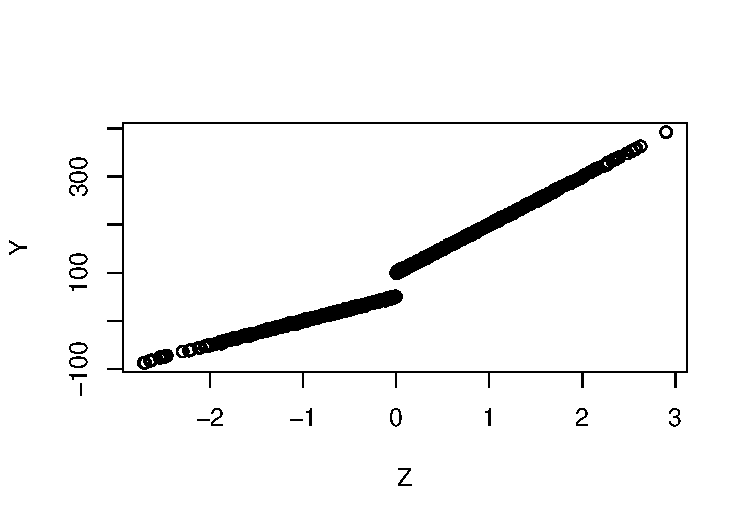
\includegraphics[width=\maxwidth]{./figures/rdd_ex_1_1-1} 

}

\caption[Exemplo em que Z satisfaz o critério backdoor para medir o efeito causal de X em Y e X = I(Z > 0)]{Exemplo em que Z satisfaz o critério backdoor para medir o efeito causal de X em Y e X = I(Z > 0). Como resultado da descontinuidade da propensidade de X em Z = 0, há uma descontinuidade na regressão E[Y|Z] no ponto Z=0.}\label{fig:rdd_ex_1_1}
\end{figure}

\end{knitrout}
 
 Como estamos simulando os dados,
 podemos calcular $\CACE(0)$:
 \begin{align*}
  \CACE(0) 
  &= \lim_{\z \downarrow 0}\E[Y|\Z=\z] 
  - \lim_{\z \uparrow 0}\E[Y|\Z=\z]
  & \text{\cref{thm:id_rdd}} \\
  &= \lim_{\z \downarrow 0}\E[Y|X=1,\Z=\z]
  - \lim_{\z \uparrow 0}\E[Y|X=0,\Z=\z] \\
  &= \lim_{\z \downarrow 0} 50(1+1)(\z+1)
  - \lim_{\z \uparrow 0} 50(0+1)(\z+1)
  = 50
 \end{align*}
\end{example}

O código abaixo estima $\CACE(0)$ usando regressão linear:

\begin{knitrout}
\definecolor{shadecolor}{rgb}{0.969, 0.969, 0.969}\color{fgcolor}\begin{kframe}
\begin{alltt}
\hlstd{regs} \hlkwb{=} \hlstd{data} \hlopt
  \hlkwd{mutate}\hlstd{(}\hlkwc{Z1} \hlstd{= (Z} \hlopt{>=} \hlnum{0}\hlstd{))} \hlopt
  \hlkwd{group_by}\hlstd{(Z1)} \hlopt
  \hlkwd{summarise}\hlstd{(}
    \hlkwc{intercepto} \hlstd{=} \hlkwd{lm}\hlstd{(Y} \hlopt{~} \hlstd{Z)}\hlopt{$}\hlstd{coefficients[}\hlnum{1}\hlstd{],}
    \hlkwc{coef_angular} \hlstd{=} \hlkwd{lm}\hlstd{(Y} \hlopt{~} \hlstd{Z)}\hlopt{$}\hlstd{coefficients[}\hlnum{2}\hlstd{]}
  \hlstd{)}
\hlstd{regs}
\end{alltt}
\begin{verbatim}
## # A tibble: 2 x 3
##   Z1    intercepto coef_angular
##   <lgl>      <dbl>        <dbl>
## 1 FALSE       50.1         50.1
## 2 TRUE        99.9        100.
\end{verbatim}
\begin{alltt}
\hlstd{est_cace} \hlkwb{=} \hlnum{1}\hlopt{*}\hlstd{regs[}\hlnum{2}\hlstd{,} \hlnum{2}\hlstd{]} \hlopt{+} \hlnum{0}\hlopt{*}\hlstd{regs[}\hlnum{2}\hlstd{,} \hlnum{3}\hlstd{]} \hlopt{-}
  \hlnum{1}\hlopt{*}\hlstd{regs[}\hlnum{1}\hlstd{,} \hlnum{2}\hlstd{]} \hlopt{+} \hlnum{0}\hlopt{*}\hlstd{regs[}\hlnum{1}\hlstd{,} \hlnum{3}\hlstd{]}
\hlkwd{round}\hlstd{(}\hlkwd{as.numeric}\hlstd{(est_cace),} \hlnum{2}\hlstd{)}
\end{alltt}
\begin{verbatim}
## [1] 49.81
\end{verbatim}
\end{kframe}
\end{knitrout}

Similarmente, podemos estimar $\CACE(0)$ usando
regressão por kernel de Nadaraya-Watson:

\begin{knitrout}
\definecolor{shadecolor}{rgb}{0.969, 0.969, 0.969}\color{fgcolor}\begin{kframe}
\begin{alltt}
\hlkwd{library}\hlstd{(np)}
\hlkwd{options}\hlstd{(}\hlkwc{np.messages} \hlstd{=} \hlnum{FALSE}\hlstd{)}
\hlstd{nw_reg} \hlkwb{<-} \hlkwa{function}\hlstd{(}\hlkwc{data}\hlstd{,} \hlkwc{valor}\hlstd{)}
\hlstd{\{}
  \hlstd{bw} \hlkwb{<-} \hlkwd{npregbw}\hlstd{(}\hlkwc{xdat} \hlstd{= data}\hlopt{$}\hlstd{Z,} \hlkwc{ydat} \hlstd{= data}\hlopt{$}\hlstd{Y)}\hlopt{$}\hlstd{bw}
  \hlkwd{npksum}\hlstd{(}\hlkwc{txdat}\hlstd{= data}\hlopt{$}\hlstd{Z,} \hlkwc{exdat} \hlstd{= valor,} \hlkwc{tydat} \hlstd{= data}\hlopt{$}\hlstd{Y,} \hlkwc{bws} \hlstd{= bw)}\hlopt{$}\hlstd{ksum}\hlopt{/}
    \hlkwd{npksum}\hlstd{(}\hlkwc{txdat} \hlstd{= data}\hlopt{$}\hlstd{Z,} \hlkwc{exdat} \hlstd{= valor,} \hlkwc{bws} \hlstd{= bw)}\hlopt{$}\hlstd{ksum}
\hlstd{\}}

\hlstd{reg_baixo} \hlkwb{<-} \hlstd{data} \hlopt
  \hlkwd{filter}\hlstd{(Z} \hlopt{<} \hlnum{0}\hlstd{)} \hlopt
  \hlkwd{nw_reg}\hlstd{(}\hlnum{0}\hlstd{)}
\hlstd{reg_cima} \hlkwb{<-} \hlstd{data} \hlopt
  \hlkwd{filter}\hlstd{(Z} \hlopt{>=} \hlnum{0}\hlstd{)} \hlopt
  \hlkwd{nw_reg}\hlstd{(}\hlnum{0}\hlstd{)}
\hlstd{est_cace} \hlkwb{<-} \hlstd{reg_cima} \hlopt{-} \hlstd{reg_baixo}
\hlkwd{round}\hlstd{(est_cace,} \hlnum{2}\hlstd{)}
\end{alltt}
\begin{verbatim}
## [1] 51.31
\end{verbatim}
\end{kframe}
\end{knitrout}

\subsection{Exercícios}

\begin{exercise}
 Crie um exemplo em que,
 ao contrário do \cref{ex:rdd},
 $\E[Y|X=1,\Z]$ não é linear em $\Z$.
 Compare as estimativas de $\CACE$ usando
 a regressão linear e 
 algum método de regressão não-paramétrica.
\end{exercise}

\section{Do-calculus}
\label{sec:do_calculus}

\begin{theorem}
 \label{thm:do_calculus}
 Teste
 \begin{enumerate}
  \item Seja $\sG^*$ o grafo obtido retirando de $\sG$ 
  todas as arestas que apontam para $\X$. 
  Se $\Y \dsep \Z | \X \cup \W$ em $\sG^*$, então
  \begin{align*}
   f(\Y|do(\X), \Z, \W) &= f(\Y|do(\X), \W)
  \end{align*}
  \item Seja $\sG^+$ o grafo obtido retirando de $\sG$ 
  todas as arestas que 
  apontam para $\X$ ou 
  que partem de $\Z$. 
  Se temos que $\Y \dsep \Z | \X \cup \W$ em $\sG^+$, então
  \begin{align*}
   f(\Y|do(\X), do(\Z), \W) &= f(\Y|do(\X), \W)
  \end{align*}
  \item 
 \end{enumerate}
\end{theorem}

\section{Controlando mediadores (critério frontdoor)}
\label{sec:frontdoor}

\begin{knitrout}
\definecolor{shadecolor}{rgb}{0.969, 0.969, 0.969}\color{fgcolor}\begin{figure}[t]

{\centering 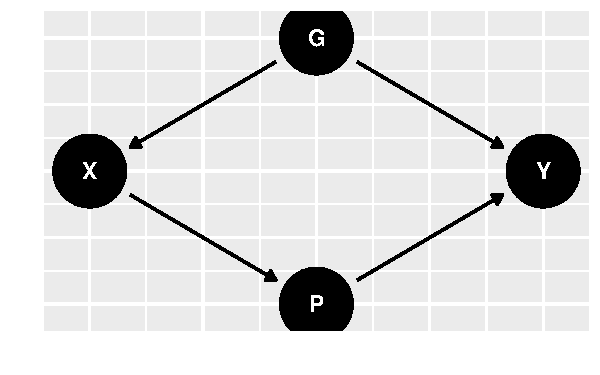
\includegraphics[width=\maxwidth]{./figures/frontdoor_ex_1-1} 

}

\caption[]{.}\label{fig:frontdoor_ex_1}
\end{figure}

\end{knitrout}

Há casos em que não existem variáveis observadas que 
satisfazem o critério backdoor.
Por exemplo, considere o grafo causal 
na \cref{fig:frontdoor_ex_1} \citep{Glymour2016}.
Neste grafo, estamos interessados em
compreender o efeito causal
do fumo ($X$) sobre a incidência de câncer ($Y$).
Além disso, fatores genéticos não observáveis ($G$)
são um potencial confundidor, uma vez que 
podem ter influência tanto sobre o fumo quanto 
sobre a incidência de câncer.
Assim, como $G$ não é observado,
não é possível implementar 
os métodos de estimação vistos na última seção.

Apesar desta dificuldade, 
ainda é possível medir o efeito causal de $X$ em $Y$
na \cref{fig:frontdoor_ex_1}.
Para tal, a estratégia é 
mensurar o efeito de 
todos os caminhos direcionados que 
partem de $X$ e chegam a $Y$.
Em outras palavras, 
a estratégia é 

\begin{align*}
 f(y|do(X)) 
 &= \int f(y|do(W))f(W|do(X))dW
\end{align*}

\begin{align*}
 \E[Y|do(X)]
 &= \int y f(y|do(X)) \\
 &= \int \int y f(y|do(W)) f(W|do(X)) dW dy
\end{align*}

\subsection{Exercícios}

\begin{exercise}[{\citet{Glymour2016}[p.48]}]
 \label{ex:d-sep}
 Considere o modelo estrutural causal
 em \cref{fig:d-sep}.
 \begin{enumerate}[label=(\alph*)]
  \item Para cada um dos pares de variáveis a seguir,
  determine um conjunto de outras variáveis que
  as d-separa: $(Z_1,W)$, $(Z_1,Z_2)$, $(Z_1,Y)$, 
  $(Z_3,W)$, e $(X,Y)$.
  \item Para cada par de variáveis no item anterior,
  determine se elas são d-separadas dado
  todas as demais variáveis.
  \item Determine conjuntos de variáveis que
  satisfazem, respectivamente, 
  o ``backdoor criterion'' e 
   o ``frontdoor criterion'' para
  estimar o efeito causal de $X$ em $Y$.
  \item Considere que para cada variável, $V$, temos que
  $V \equiv \beta_V \cdot Pa(V) + \epsilon_V$,
  onde os $\epsilon$ são i.i.d. e normais padrão e
  $\beta_V$ são vetores conhecidos. Isto é,
  a distribuição de cada variável é 
  determinada através de 
  uma regressão linear simples em seus pais.
  Determine $f(Y|do(X=x))$ utilizando a fórmula do ajuste
  nos $2$ casos abordados no item anterior.
 \end{enumerate}
\begin{figure}
 \centering
 \tikz{
    \node (z1) {$Z_1$};
    \node (z3) [below right = of z1] {$Z_3$};
    \node (z2) [above right = of z3] {$Z_2$};
    \node (x) [below left = of z3] {$X$};
    \node (w1) [right = of x] {$W_1$};
    \node (w2) [below = of w1] {$W_2$};
    \node (y) [right = of w1] {$Y$};
    \path (z1) edge (z3);
    \path (z1) edge (x);
    \path (z2) edge (z3);
    \path (z2) edge (y);
    \path (z3) edge (x);
    \path (z3) edge (y);
    \path (x) edge (w1);
    \path (w1) edge (y);
    \path (x) edge (w2);
    \path (w2) edge (y);
}
 \caption{Modelo estrutural causal do \cref{ex:d-sep}}
 \label{fig:d-sep}
\end{figure}
\end{exercise}

\begin{exercise}
 Considere que $\sG = (\sV, \sE)$ é um grafo causal e
 $\X,\W,\Y \subseteq \sV$. Além disso,
 para todo caminho, $C = (C_1,\ldots,C_n)$,
 com $C_1 = X \in \X$, $C_n = Y \in \Y$, e
 com $X \rightarrow C_2$,
 $C$ está bloqueado dado $\W$.
 Prove que $f(\y|do(\X)) 
 = \int f(\y|\w)f(\w|do(\X))d\w$ e
 $\E[Y|do(\X)] = \E[\E[Y|\W]|do(\X)]$.
\end{exercise}

\bibliographystyle{apalike}
\bibliography{book}


\appendix

\chapter{Demonstrações}

\section{Relativas à \text{\cref{sec:d-sep}}}

\subsection{Relativas ao \cref{lemma:equivIndep}}

\begin{proof}[Prova do \cref{lemma:equivIndep}]
 A prova consistirá em demonstrar que,
 para cada $i$, a afirmação $i$ decorre da afirmação $i-1$.
 Finalmente, a afirmação $1$ decorre da afirmação $4$.
 Os símbolos $\X$ e $\x$ referem-se a 
 $(\X_1,\ldots,\X_d)$ e $(\x_1,\ldots,\x_d)$. 
 \begin{itemize}
  \item $(1 \Longrightarrow 2)$
	\begin{align*}
	 f(\x|\y)	&= \prod_{j=1}^{d}{f(\x_j|\y)}  & (1) \\
	          &= \prod_{j=1}^{d}{h(\x_j,\y)}
	          & h(\x_j,\y) = f(\x_j|\y)
	\end{align*}
	\vspace{-5mm}
  \item $(2 \Longrightarrow 3)$ Note que,
	\begin{align*}
	 f(\x_i|\x_{-i},\y)	
	 &= \frac{f(\x|\y)}{f(\x_1,\ldots,\x_{i-1},\x_{i+1},\ldots\x_d|\y)}	\\
	 &= \frac{f(\x|\y)}{\int_{\mathbb{R}}{f(\x|\y)d\x_i}} \\
	 &= \frac{\prod_{j=1}^{d}{h_j(\x_j,\y)}}
	 {\int_{\mathbb{R}}{\prod_{j=1}^{d}{h_j(\x_j,\y)}d\x_i}} (2) \\
	 &= \frac{\prod_{j=1}^{d}{h_j(\x_j,\y)}}
	 {\prod_{j \neq i}{h_j(\x_j,\y)} \int_{\mathbb{R}}{h_i(\x_i,\y)d\x_i}}	\\
	 &= \frac{\tilde{h}_i(\x_i,\y)}{\int_{\mathbb{R}}{h_i(\x_i,\y)d\x_i}}	\\
	 &= \frac{\prod_{j \neq i}{\int_{\mathbb{R}}{h_j(\x_j,\y)d\x_j}}}
	 {\prod_{j \neq i}{\int_{\mathbb{R}}{h_j(\x_j,\y)d\x_j}}} \cdot 
	 \frac{h_i(\x_i,\y)}{\int_{\mathbb{R}}{h_i(\x_i,\y)d\x_i}}	\\
	 &= \frac{\int_{\mathbb{R}^{d-1}}{\prod_{j=1}^{d}{h_j(\x_j,\y)}d\x_{-i}}}
	 {\int_{\mathbb{R}^{d}}{\prod_{j=1}^{d}{h_j(\x_j,\y)}d\x}}	\\
	 &= \frac{\int_{\mathbb{R}^{d-1}}{f(\x|\y)d\x_{-i}}}
	 {\int_{\mathbb{R}^{d}}{f(\x|\y)d\x}} & (2) \\
	 &= f(\x_i|\y)
	\end{align*}

 \vspace{-5mm}
 \item $(3 \Longrightarrow 4)$
 \begin{align*}
  f(\x_i|\x_1^{i-1},\y)	
  &= \frac{f(\x_1^{i}|\y)}{f(\x_1^{i-1}|\y)} \\
	&= \frac{\int_{\mathbb{R}^{d-i}}{f(\x|\y)}d\x_{i+1}^{d}}
	{f(\x_1^{i-1}|\y)} \\
	&= \frac{\int_{\mathbb{R}^{d-i}}{f(\x_{-i}|\y)f(\x_i|\x_{-i},\y)d\x_{i+1}^{d}}}
	{f(\x_1^{i-1}|\y)} \\
	&= \frac{f(\x_i|\y)\int_{\mathbb{R}^{d-i}}{f(\x_{-i}|\y)d\x_{i+1}^{d}}}
	{f(\x_1^{i-1}|\y)} & (3) \\
	&= \frac{f(\x_i|\y)f(\x_1^{i-1}|\y)}
	{f(\x_1^{i-1}|\y)} \\
	&= f(\x_i|\y)
 \end{align*}

 \item $(4 \Longrightarrow 1)$
 \begin{align*}
  f(\x|\y)	
  &= \prod_{i=1}^{d}{f(\x_i|\x_1^{i-1},\y)} \\
	&= \prod_{i=1}^{d}{f(\x_i|\y)} & (4)
 \end{align*}
 \end{itemize}
\end{proof}

\subsection{Relativas ao \cref{thm:d-sep}}

\begin{lemma}
 \label{lem:dsep_indep_anc}
 Seja $\sG = (\sV, \sE)$ um DAG.
 Se $\sA = \V_1 \cup \V_2 \cup \V_3$ é ancestral e
 $\V_1 \perp \V_2 | \V_3$, então, 
 para todo $f$ compatível com $\sG$,
 $\V_1 \ind^f \V_2 | \V_3$.
\end{lemma}

\begin{proof}
 Defina $\V^*_1 = \{V \in \sA: 
 V \in \V_1 \text{ ou } V_1 \rightarrow V,
 \text{ para algum } V_1 \in \V_1\}$ e
 $\V^*_2 = \sA - \V^*_1$.
 Como $\V_1 \perp \V_2 | \V_3$, decorre de
 \cref{def:d-sep} que não existe
 $V_1 \in \V_1$ e $V_2 \in \V_2$ tal que
 $V_1 \rightarrow V_2$. Portanto,
 \begin{align}
  \label{eq:d_sep_tot_1}
  \V^*_1 \subseteq \V_1 \cup \V_3 \text{ e }
  \V^*_2 \subseteq \V_2 \cup \V_3
 \end{align}
 A seguir, demonstraremos que
 \begin{align}
  \label{eq:d_sep_tot_2}
  \forall i \in \{1,2\} \text{ e }
  V^*_i \in \V^*_i:
  Pa(V^*_i) \subseteq \V_i \cup \V_3
 \end{align}
 Tome $V^*_1 \in \V^*_1$.
 Como $V^*_1 \in \sA$ e $\sA$ é ancestral,
 decorre da \cref{def:ancestral} que
 $Pa(V^*_1) \subseteq \sA$.
 Assim, basta demonstrar que 
 $Pa(V^*_1) \cap \V_2 = \emptyset$. 
 Se $V^*_1 \in \V_1$, então decorre de
 \cref{def:d-sep} que não existe
 $V_2 \in \V_2$ tal que $V_2 \rightarrow V^*_1$.
 Caso contrário, se $V^*_1 \in \V_3$,
 então existe $V_1 \in \V_1$ tal que
 $V_1 \rightarrow V^*_1$.
 Decorre de \cref{def:d-sep} que não existe 
 $V_1 \in \V_1$, $V_2 \in \V_2$ e
 $V_3 \in \V_3$ tais que $V_3$ é
 um colisor entre $V_1$ e $V_2$, isto é,
 $V_1 \rightarrow V_3 \leftarrow V_2$.
 Portanto, não existe $V_2 \in \V_2$ tal que
 $V_2 \rightarrow V^*_1$.
 Conclua que $Pa(V^*_1) \subseteq \V_1 \cup \V_3$.
 
 A seguir, note que 
 pela definição de $\V^*_1$, 
 se $V \in \sA$ é tal que
 existe $V_1 \in \V_1$ com
 $V_1 \rightarrow V$, então
 $V \in \V^*_1$. Portanto,
 como $\V^*_2 = \sV - \V^*_1$, 
 para todo $V^*_2 \in \V^*_2$,
 não existe $V_1 \in \V_1$ tal que
 $V_1 \rightarrow V^*_2$.
 Isto é, $Pa(V^*_2) \subseteq \sV - \V_1$.
 Como $V^*_2 \in \sA$ e $\sA$ é ancestral,
 conclua da \cref{def:ancestral} que
 $Pa(V^*_2) \subseteq \sA$.
 Combinando as duas últimas frases,
 $Pa(V^*_2) \subseteq \V_2 \cup \V_3$.
 
 Decorre da conclusão dos dois últimos parágrafos que
 \cref{eq:d_sep_tot_2} está demonstrado.
 \begin{align*}
  f(\V_1,\V_2|\V_3)
  &= \frac{f(\V_1,\V_2,\V_3)}{f(\V_3)} \\
  &= \frac{\prod_{V \in \sA}f(V|Pa(V))}
  {f(\V_3)} 
  & \text{\cref{lem:anc_fat}} \\
  &= \frac{\left(\prod_{V^*_1 \in \V^*_1}
  f(V^*_1|Pa(V^*_1))\right)
  \left(\prod_{V^*_2 \in \V^*_2}
  f(V^*_2|Pa(V^*_2))\right)}
  {f(\V_3)} 
  & \V^*_1 \text{ e } \V^*_2 \text{ particionam } \sA \\
  &= h_1(\V_1, \V_3) h_2(\V_2, \V_3)
  & \text{\cref{eq:d_sep_tot_1,eq:d_sep_tot_2}}
 \end{align*}
 Assim, decorre do \cref{lemma:equivIndep} que
 $\V_1 \ind^f \V_2 | \V_3$.
\end{proof}

\begin{lemma}
 \label{lem:dsep_indep}
 Se $f$ é compatível com $\sG$ e
 $\V_1 \perp \V_2 | \V_3$, então
 $\V_1 \ind^f \V_2 | \V_3$.
\end{lemma}

\begin{proof}
 Defina $\sA = Anc(\V_1 \cup \V_2 \cup \V_3)$,
 $\V^*_1 = \{V \in \sA: V \text{ não é d-separado de } \V_1 | \V_3\}$, e $\V^*_2 = \sA - \V^*_1$.
 Por definição,
 \begin{align}
  \label{eq:dsep_indep_0}
  \V_1 \subseteq \V^*_1 \text{ e }
  \V_2 \subseteq \V^*_2
 \end{align}

 O primeiro é provar que
 $\V^*_1 \perp \V^*_2 | \V_3$.
 Pela definição de $\V^*_2$, 
 para todo $V_1 \in \V_1$ e $V^*_2 \in \V^*_2$, 
 $V_1 \perp V^*_2 | \V_3$, isto é,
\begin{align}
 \label{eq:dsep_indep_1}
 \V_1 \perp \V^*_2 | \V_3
\end{align}
 Suponha por absurdo que existam
 $V^*_1 \in \V^*_1$ e $V^*_2 \in \V^*_2$
 tais que $V^*_1$ e $V^*_2$ 
 não são d-separados dado $\V_3$.
 Portanto, existe um caminho ativo dado $\V_3$,
 $(V^*_1,C_2,\ldots,C_{n-1},V^*_2)$.
 Pela definição de $\V^*_1$, existe
 $V_1 \in \V_1$ e um caminho ativo dado $\V_3$,
 $(V_1,C^*_2,\ldots,C^*_{m-1},V^*_1)$. Assim,
 $(V_1,C^*_2,\ldots,C^*_{m-1},
 V^*_1,C_2,\ldots,C_{n-1},V^*_2)$ é
 é um caminho ativo dado $\V_3$ de
 $V_1$ a $V^*_2$, uma contradição com
 \cref{eq:dsep_indep_1}. Conclua que
 $\V^*_1 \perp \V^*_2 | \V_3$.

 A seguir, provaremos que
 $\V^*_1 \ind^f \V^*_2 | \V_3$.
 Como $\sA = Anc(\V_1 \cup \V_2 \cup \V_3)$,
 decorre do \cref{lem:anc} que
 $\sA$ é ancestral. Portanto, como
 $\sA = \V^*_1 \cup \V^*_2 \cup \V_3$ e
 $\V^*_1 \perp \V^*_2 | \V_3$, decorre do
 \cref{lem:dsep_indep_anc} que
 $\V^*_1 \ind^f \V^*_2 | \V_3$.

Como $\V^*_1 \ind^f \V^*_2 | \V_3$,
 a conclusão do lema decorre do fato de que
 $\V_1 \subseteq \V^*_1$ e 
 $\V_2 \subseteq \V^*_2$. 
\end{proof}

\begin{lemma}
 \label{lemma:d-sep-volta}
 Se $\V_1$ não é d-separado de $\V_2$
 dado $\V_3$ segundo o DAG $\sG = (\sV, \sE)$, então
 existe $f$ compatível com $\sG$ tal que
 $\V_1$ e $\V_2$ são condicionalmente dependentes
 dado $\V_3$ segundo $f$
\end{lemma}

\begin{proof}
\end{proof}

\begin{proof}[Prova do \cref{thm:d-sep}]
 Decorre dos 
 \cref{lem:dsep_indep,lemma:d-sep-volta}.
\end{proof}

\section{Relativas à \cref{sec:backdoor}}

\subsection{Relativas ao \cref{thm:backdoor}}

Para realizar a demonstração do \cref{thm:backdoor},
consideraremos um SCM aumentado, 
em que existe uma variável que representa
a ocorrência de uma intervenção em X.
Uma consequência interessante desta construção será
a de que o modelo intervencional é equivalente
ao condicionamento usual no SCM aumentado.

\begin{definition}
 \label{def:scm_star}
 Seja $(\sG_*, f_*)$ um SCM expandido tal que
 $\sG_* = (\sV \cup \{I\}, \sE_*)$, e
 $\sE_* = \sE \cup \{(I \rightarrow X)\}$.
 Isto é, $\sG_*$ é uma cópia de $\sG$ em que
 adicionamos o vértice $I \in \{0,1\}$ e 
 uma única aresta de $I$ para $X$.
 
 $\sG^*$ admite uma interpretação intuitiva.
 $I$ é a indicadora de que fazemos uma intervenção em $X$,
 fazendo que esta assuma o valor $x$.
 Se $I = 0$, não há uma intervenção e, assim,
 $X$ segue a sua distribuição observacional.
 Se $I = 1$, $X$ assume o valor $x$ com probabilidade $1$.
 
 Finalmente, considerando $Pa(X)$ como os
 pais de $X$ segundo $\sG$, definimos que:
 \begin{align*}
  f_*(X|Pa(X), I) 
  &= \begin{cases}
   f(X|Pa(X)) & \text{, se $I = 0$, e} \\
   \I(X = x) & \text{, caso contrário.}
  \end{cases}
 \end{align*}
\end{definition}

\begin{lemma}
 \label{lemma:backdoor_1}
 Se $(\sG^*, f^*)$ é tal qual em \cref{def:scm_star}, então:
 \begin{align*}
  f(y|do(X=x)) &= f_*(y|I=1)
 \end{align*}
\end{lemma}

\begin{proof}
 Tomando $\V_2 = \sV - \{X\}$:
 \begin{align*}
  f_*(\V_2|I = 1) 
  &= \frac{f_*(\V_2, I=1)}{f(I=1)} \\
  &= \frac{\int f_*(\V_2, X, I=1)dX}{f(I=1)} \\
  &= \frac{f(I=1)\I(X = x)\prod_{V_2 \in \V_2}f(V_2|Pa(V_2))}{f(I=1)}
  & \text{\cref{def:scm_star}} \\
  &= \I(X = x) \cdot \prod_{V_2 \in \V_2}f(V_2|Pa(V_2)) \\
  &= f(\V_2|do(X=x)) 
  & \text{\cref{def:intervencao}}
 \end{align*}
\end{proof}

\begin{lemma}
 \label{lemma:backdoor_2}
 Se $(\sG^*, f^*)$ é tal qual em \cref{def:scm_star}, então:
 \begin{align*}
  f_*(\sV|I=0) &= f(\sV).
 \end{align*}
\end{lemma}

\begin{proof}
 \begin{align*}
  f_*(\sV|I=0) 
  &= \frac{f_*(\sV, I=0)}{f_*(I=0)} \\
  &= \frac{f_*(I=0)f_*(X|Pa(X),I=0)
  \prod_{V \in \sV-\{X\}} f(V|Pa(V))}{f_*(I=0)}
  & \text{\cref{def:scm_star}} \\
  &= f(X|Pa(X))\prod_{V \in \sV-\{X\}} f(V|Pa(V))
  & \text{\cref{def:scm_star}} \\
  &= \prod_{V \in \sV} f(V|Pa(V)) \\
  &= f(\sV) 
  & \text{\cref{def:compativel}}
 \end{align*}
\end{proof}

\begin{lemma}
 \label{lemma:backdoor_3}
 Se $(\sG^*, f^*)$ é tal qual em \cref{def:scm_star} e
 $\Z$ satisfaz o critério backdoor para
 medir o efeito causal de $X$ em $Y$, então $I \dsep Y | X, \Z$.
\end{lemma}

\begin{proof}
 Tome um caminho arbitrário de
 $I$ em $Y$, $C = (I, C_2, \ldots, C_{n-1}, Y)$.
 Por definição de $I$, $C_2 = X$ e 
 $I \rightarrow X$. 
 Se $X \rightarrow C_3$, então
 $X$ é uma cadeia em $C$ e 
 $C$ está bloqueado dado $X$ e $\Z$.
 Se $X \leftarrow C_3$, então
 $(X, C_3, \ldots, C_{n-1}, Y)$ está bloqueado
 dado $\Z$, uma vez que $\Z$ satisfaz
 o critério backdoor.
 Conclua que $C$ está bloqueado dado $X$ e $\Z$.
\end{proof}

\begin{lemma}
 \label{thm:backdoor_pt_1}
 Se $\Z$ satisfaz o critério backdoor para
 medir o efeito causal de $X$ em $Y$, então
 $f(y|do(x),\z) = f(y|x,\z)$.
\end{lemma}

\begin{proof}
 \begin{align*}
  f(y|do(x),\z)
  &= f_*(y|I=1, \z)
  & \text{\cref{lemma:backdoor_1}} \\
  &= \int f_*(y,X|I=1, \z)dX \\
  &= \int f_*(X|I=1,\z)f_*(y|X, I=1, \z)dX \\
  &= \int \I(X=x)f_*(y|X, I=1, \z)dX \\
  &= f_*(y|x,I=1,\z) \\
  &= f_*(y|x,I=0,\z)
  & \text{\cref{lemma:backdoor_3}} \\
  &= f(y|x,\z)
  & \text{\cref{lemma:backdoor_2}}
 \end{align*}
\end{proof}

\begin{lemma}
 \label{lemma:backdoor_4}
 Se $(\sG^*, f^*)$ é tal qual em \cref{def:scm_star} e
 $\X \notin Anc(\Z)$, então:
 \begin{align*}
  f_*(\z) &= f(\z)
 \end{align*}
\end{lemma}

\begin{proof}
 Seja $\Z_* = Anc(\Z)$ e
 $\V = \sV - (\{X\} \cup \Z_*)$.
 Como $X \notin \Z_*$, decorre 
 da \cref{def:scm_star} que $I \notin \Z_*$.
 Portanto,
 \begin{align*}
  f_*(\z_*) 
  &= \int f_*(\z_*, I,X,\bv) d(I,X,\bv) \\
  &= \int \left(\prod_{z \in \z_*} f(z|Pa(z))\right)
  \left(f_*(I)f_*(X|I,Pa(X))
  \prod_{v \in \bv} f(v|Pa(v))\right)d(I,X,\bv)
  & \text{\cref{def:scm_star}} \\
  &= \left(\prod_{z \in \z_*} f(z|Pa(z))\right) 
  \int \left(f_*(I)f_*(X|I,Pa(X)) 
  \prod_{v \in \bv} f(v|Pa(v))\right)d(I,X,\bv) 
  & \Z_* \cap (\V \cup \{I,X\}) = \emptyset \\
  &\propto \prod_{z \in \z_*} f(z|Pa(z)) 
  & \Z_* \cap (\V \cup \{I,X\}) = \emptyset \\
  &= f(\z_*) 
  & \text{\cref{lemma:anc_fact}}
 \end{align*}
 Assim, decorre da Lei da Probabilidade Total que
 $f_*(\z) = f(\z)$.
\end{proof}

\begin{lemma}
 \label{lemma:backdoor_5}
 Se $(\sG^*, f^*)$ é tal qual em \cref{def:scm_star} e
 $\Z$ satisfaz o critério backdoor para
 medir o efeito causal de $X$ em $Y$, então $I \dsep \Z$.
\end{lemma}

\begin{proof}
 Tome arbitrariamente um $Z \in \Z$ e
 um caminho de $I$ em $Z$, 
 $C = (I, C_2, \ldots, C_{n-1}, Z)$.
 Por definição de $I$, $C_2 = X$ e
 $I \rightarrow X$. 
 Suponha por absurdo que $C$ não tem colisor.
 Como, $I \rightarrow X$, decorre que
 $C = I \rightarrow X \rightarrow \ldots 
 \rightarrow C_{n-1} \rightarrow Z$.
 Assim, $Z$ é um descendente de $X$,
 uma contradição com 
 o critério backdoor (\cref{def:backdoor}).
 Conclua que $C$ tem um colisor.
 Assim, $C$ está marginalmente bloqueado
 (\cref{def:caminho-bloq}).
\end{proof}

\begin{lemma}
 \label{thm:backdoor_pt_2}
 Se $\Z$ satisfaz o critério backdoor para
 medir o efeito causal de $X$ em $Y$, então
 $f(\z|do(x)) = f(\z)$.
\end{lemma}

\begin{proof}
 \begin{align*}
  f(\z|do(x))
  &= f_*(\z|I=1)
  & \text{\cref{lemma:backdoor_1}} \\
  &= f_*(\z)
  & \text{\cref{lemma:backdoor_5}} \\
  &= f(\z)
  & \text{\cref{lemma:backdoor_4}}
 \end{align*}
\end{proof}

\begin{proof}[Prova do \cref{thm:backdoor}]
 Decorre diretamente dos
 \cref{thm:backdoor_pt_1,thm:backdoor_pt_2}.
\end{proof}

\begin{proof}[Prova do \cref{cor:backdoor}]
 \begin{align*}
  f(y|do(X=x))
  &= \int f(y,\z|do(X=x))d\z \\
  &= \int f(\z|do(X=x))f(y|do(X=x),\z) \\
  &= \int f(\z)f(y|x,\z)
  & \text{\cref{thm:backdoor}}
 \end{align*}
\end{proof}

\subsection{Relativas aos \cref{thm:backdoor_ajuste,thm:backdoor_ipw}}

\begin{proof}[Prova do \cref{thm:backdoor_ajuste}]
 \begin{align}
  \label{eq:backdoor_ajuste_1}
  \E[g(Y)|do(X=x),\Z]
  &= \int g(y) f(y|do(x),\Z) dy 
  & \text{\cref{def:exp_inter}} \nonumber \\
  &= \int g(y) f(y|x, \Z)dy 
  & \text{\cref{thm:backdoor}} \nonumber \\
  &= \E[g(Y)|X=x,\Z] \\
  \E[g(Y)|do(X=x)]
  &= \E[\E[g(Y)|do(X=x),\Z]] \nonumber \\
  &= \E[\E[g(Y)|X=x,\Z]]
  & \text{\cref{eq:backdoor_ajuste_1}} \nonumber
 \end{align}
\end{proof}

\begin{proof}[Prova do \cref{thm:backdoor_ipw}]
 \begin{align*}
  \E[g(Y)|do(x),\Z]
  &= \int g(y) f(y|do(x),\Z) dy
  & \text{\cref{def:exp_inter}} \\
  &= \int g(y) f(y|x,\Z) dy
  & \text{\cref{thm:backdoor}} \\
  &= \int \frac{g(y) f(y,x|\Z)}{f(x|\Z)} dy \\
  &= \int \frac{g(y) \I(x_* = x) f(y,x_*|\Z)}{f(x|\Z)} d(x_*, y) \\
  &= \E\left[\frac{g(Y)\I(X=x)}{f(x|\Z)}|\Z\right] \\
  &= \frac{\E[g(Y)\I(X=x)|\Z]}{f(x|\Z)}
 \end{align*}
 \begin{align*}
  \E[Y|do(x)]
  &= \E[\E[Y|do(X),\Z]] \\
  &= \E\left[\frac{\E[g(Y)\I(X=x)|\Z]}{f(x|\Z)}\right] 
  & \text{\cref{thm:backdoor_ipw}} \\
  &= \E\left[\E\left[\frac{g(Y)\I(X=x)}{f(x|\Z)}|\Z\right]\right] \\
  &= \E\left[\frac{g(Y)\I(X=x)}{f(x|\Z)}\right]
 \end{align*}
\end{proof}

\subsection{Relativas ao \cref{thm:conv_ajuste}}

\begin{lemma}
 \label{lemma:conv_l1_to_p}
 Se $(W_n)_{n \in \mathbb{N}}$ é uma sequência de
 variáveis aleatórias tais que $\E[|W_n|] = o(1)$,
 então $W_n \convp 0$.
\end{lemma}

\begin{proof}
 \begin{align*}
  \P(|W_n| > \epsilon)
  &\leq \frac{\E[|W_n|]}{\epsilon} & \text{Markov} \\
  &= o(1)
 \end{align*}
\end{proof}

\begin{proof}[Prova do \cref{thm:conv_ajuste}]
 Como $\E[|\mu(x,\Z)|] < \infty$,
 pela Lei dos Grandes Números,
 \begin{align*}
  \frac{\sum_{i=1}^n \mu(x,\Z_i)}{n}
  &\convp \E[\mu(x,\Z)]
 \end{align*}
 Portanto, pelo \cref{thm:backdoor_ajuste},
 é suficiente provar que
 $\hdoy - \frac{\sum_{i=1}^n \mu(x,\Z_i)}{n} \convp 0$.
 Usando o \cref{lemma:conv_l1_to_p}, é suficiente provar que 
 $\E\left[\bigg|\hdoy - \frac{\sum_{i=1}^n \mu(x,\Z_i)}{n}\bigg|\right] 
 = o(1)$.
 \begin{align*}
  \E\left[\bigg|\hdoy - \frac{\sum_{i=1}^n \mu(x,\Z_i)}{n}\bigg|\right]
  &= \E\left[\bigg|\frac{\sum_{i=1}^n 
  (\hat{\mu}(x,\Z_i)-\mu(x,\Z_i))}{n}\bigg|\right] \\
  &\leq n^{-1}\sum_{i=1}^n \E\left[| 
  \hat{\mu}(x,\Z_i)-\mu(x,\Z_i)|\right] \\
  &= \E\left[|\hat{\mu}(x,\Z)-\mu(x,\Z)|\right] 
  & \text{\cref{def:perm}} \\
  &= o(1)]
 \end{align*}
\end{proof}

\subsection{Relativas ao \cref{thm:conv_ipw}}

\begin{proof}[Prova do \cref{thm:conv_ipw}]
 Pela Lei dos Grandes números,
 $n^{-1} \sum_{i=1}^n \frac{Y_i \I(X_i = x)}{f(x|\Z_i)} 
 \convp \E\left[\frac{Y \I(X = x)}{f(x|\Z)}\right]$. Como
 pelo \cref{thm:backdoor_ipw} temos que
 $\E\left[\frac{Y \I(X = x)}{f(x|\Z)}\right] = \E[Y|do(X=x)]$,
 usando o \cref{lemma:conv_l1_to_p} é suficiente provar que 
 \begin{align*}
 \E\left[\bigg|n^{-1} \sum_{i=1}^n \frac{Y_i \I(X_i = x)}{\hf(x|\Z_i)} 
  - n^{-1} \sum_{i=1}^n \frac{Y_i \I(X_i = x)}{f(x|\Z_i)}\bigg|\right]
  &= o(1).
 \end{align*}
 \begin{align*}
  &\E\left[\bigg|n^{-1} \sum_{i=1}^n \frac{Y_i \I(X_i = x)}{\hf(x|\Z_i)} 
  - n^{-1} \sum_{i=1}^n \frac{Y_i \I(X_i = x)}{f(x|\Z_i)}\bigg|\right] \\
  \leq& n^{-1}\sum_{i=1}^n
  \E\left[\bigg|\frac{Y_i \I(X_i = x)}{\hf(x|\Z_i)} 
  -\frac{Y_i \I(X_i = x)}{f(x|\Z_i)}\bigg|\right] \\
  =& \E\left[\bigg|\frac{Y_1 \I(X_1 = x)}{\hf(x|\Z_1)} 
  -\frac{Y_1 \I(X_1 = x)}{f(x|\Z_1)}\bigg|\right]
  & \text{\cref{def:perm}} \\
  =& \E\left[\bigg|\frac{Y_i \I(X_i = x)(\hf(x|\Z_i)-f(x|\Z_i))}
  {\hf(x|\Z_i)f(x|\Z_i)}\bigg|\right] \\
  \leq& \delta^{-2}\E\left[|Y_i \I(X_i = x)(\hf(x|\Z_i)-f(x|\Z_i))|\right] 
  & \inf_z \min\{f(x|\Z_1), \hf(x|\Z_1)\} > \delta \\
  =& \delta^{-2}\E\left[|
  \hf(x|\Z_i)-f(x|\Z_i)|\cdot \E[|Y_i \I(X_i = x)|\big|\Z]\right] 
  & \text{Lei da esperança total} \\
  \leq& M\delta^{-2} \E\left[|\hf(x|\Z_i)-f(x|\Z_i)|\right]
  & \sup_z \E[|Y_i \I(X_i = x)|\Z=\z] < M \\
  =& o(1)
 \end{align*}
\end{proof}

\subsection{Relativas ao \cref{thm:conv_duplo_robusto}}

\begin{proof}[Prova do \cref{thm:conv_duplo_robusto}]
 Se as condições do \cref{thm:conv_ajuste} estão satisfeitas,
 então decorre deste resultado que 
 $\hdoy \convp \E[Y|do(X=x)]$. Portanto, 
 usando \cref{lemma:conv_l1_to_p}, 
 resta demonstrar que
 \begin{align*}
  \E\left[\bigg|\hdoyb 
  -\sum_{i=1}^n \frac{\I(X_i=x)\hat{\mu}(x,\Z_i)}
  {n\hat{f}(x|\Z_i)}\bigg|\right]
  &= o(1)
 \end{align*}
 \begin{align*}
  &\E\left[\bigg|\hdoyb 
  -\sum_{i=1}^n \frac{\I(X_i=x)\hat{\mu}(x,\Z_i)}
  {n\hat{f}(x|\Z_i)}\bigg|\right] \\
  =& \E\left[\bigg|\sum_{i=1}^n \frac{\I(X_i=x)(Y_i-\hat{\mu}(x,\Z_i))}
  {n\hat{f}(x|\Z_i)}\bigg|\right]
  & \text{\cref{def:ipw}} \\
  \leq& n{-1}\sum_{i=1}^n
  \E\left[\bigg|\frac{\I(X_i=x)(Y_i-\hat{\mu}(x,\Z_i))}
  {\hat{f}(x|\Z_i)}\bigg|\right] \\
  =& \E\left[\bigg|\frac{\I(X_1=x)(Y_1-\hat{\mu}(x,\Z_1))}
  {\hat{f}(x|\Z_1)}\bigg|\right]
  & \text{\cref{def:perm}} \\
  \leq& \delta^{-1}
  \E\left[\big|\I(X_1=x)(Y_1-\hat{\mu}(x,\Z_1))
  \big|\right]
  & \inf_\z \hf(x|\z) > \delta \\
  \leq& \delta^{-1}
  \E\left[\big|\I(X_1=x)(\E[Y_1|X_1,\Z_1]-\hat{\mu}(x,\Z_1))
  \big|\right]
  & \text{Lei da esperança total} \\
  =& \delta^{-1}
  \E\left[\big|\I(X_1=x)(\E[Y_1|X_1=x,\Z_1]-\hat{\mu}(x,\Z_1))
  \big|\right]
  & \I(X_1=x)\E[Y_1|X_1,\Z_1] 
  \equiv \I(X_1=x)\E[Y_1|X_1=x,\Z_1] \\
  \leq&\delta^{-1}
  \E\left[\big|\E[Y_1|X_1=x,\Z_1]-\hat{\mu}(x,\Z_1)
  \big|\right] \\
  =& \E\left[\big|\mu(x,\Z_1)-\hat{\mu}(x,\Z_1)
  \big|\right] = o(1)
 \end{align*}
 A seguir, se as condições do 
 \cref{thm:conv_ipw} estão satisfeitas,
 então decorre deste resultado que 
 $\hdoyb \convp \E[Y|do(X=x)]$.
 Portanto, 
 usando \cref{lemma:conv_l1_to_p}, 
 resta demonstrar que
 \begin{align*}
  \E\left[\bigg|\hdoy 
  -\sum_{i=1}^n \frac{\I(X_i=x)\hat{\mu}(x,\Z_i)}
  {n\hat{f}(x|\Z_i)}\bigg|\right]
  &= o(1)
 \end{align*}
 \begin{align*}
  &\E\left[\bigg|\hdoy 
  -\sum_{i=1}^n \frac{\I(X_i=x)\hat{\mu}(x,\Z_i)}
  {n\hat{f}(x|\Z_i)}\bigg|\right] \\
  =& \E\left[\bigg|\sum_{i=1}^n 
  \frac{(\hf(x|\Z_i)-\I(X_i=x))
  \hat{\mu}(x,\Z_i)}
  {n\hf(x|\Z_i)}\bigg|\right]
  & \text{\cref{def:ajuste}} \\
  \leq& n^{-1}\sum_{i=1}^n\E\left[\bigg| 
  \frac{(\hf(x|\Z_i)-\I(X_i=x))
  \hat{\mu}(x,\Z_i)}
  {\hf(x|\Z_i)}\bigg|\right] \\
  =& \E\left[\bigg| 
  \frac{(\hf(x|\Z_1)-\I(X_1=x))
  \hat{\mu}(x,\Z_1)}
  {\hf(x|\Z_1)}\bigg|\right] 
  & \text{\cref{def:perm}} \\
  \leq& \delta^{-1} \E\left[\big| 
  (\hf(x|\Z_1)-\I(X_1=x))
  \hat{\mu}(x,\Z_1)\big|\right] 
  & \inf_\z \hf(x|\Z_1) > \delta \\
  \leq& \delta^{-1}M \E\left[\big| 
  \hf(x|\Z_1)-\I(X_1=x)\big|\right] 
  & \sup_\z \hat{\mu}(x,\z) < M \\
  =& \delta^{-1}M \E\left[\big| 
  \hf(x|\Z_1)-\E[\I(X_1=x)|\Z_1]\big|\right] 
  & \text{Lei da esperança total} \\
  =& \delta^{-1}M \E\left[\big| 
  \hf(x|\Z_1)-f(x|\Z_1)\big|\right]
  = o(1)
 \end{align*}
\end{proof}

\subsection{Relativas ao \cref{thm:id_rdd}}

\begin{proof}[Prova do \cref{thm:id_rdd}]
 Se $X \equiv \I(\Z \geq \z_1)$, então:
 \begin{align*}
  \CACE(\Z=\z_1)
  &= \E[Y|do(X=1),\Z=\z_1] - \E[Y|do(X=0),\Z=\z_1] 
  & \text{\cref{def:cace}} \\
  &= \lim_{\z \downarrow \z_1} \E[Y|do(X=1),\Z=\z] 
  - \lim_{\z \uparrow \z_1}\E[Y|do(X=0),\Z=\z]
  & \text{continuidade} \\
  &= \lim_{\z \downarrow \z_1} \E[Y|X=1,\Z=\z] 
  - \lim_{\z \uparrow \z_1}\E[Y|X=0,\Z=\z]
  & \text{\cref{thm:backdoor_ajuste}} \\
  &= \lim_{\z \downarrow \z_1} \E[Y|X=1,\Z=\z] 
  - \lim_{\z \uparrow \z_1}\E[Y|X=0,\Z=\z]
  & X \equiv \I(\Z \geq \z_1)
 \end{align*}
 
 A seguir, considere que
 $f(x|\Z) \in (0,1)$ é contínua exceto em $\z_1$.
 Primeiramente, note que
 \begin{align}
  \label{eq:rdd_1}
  \E[Y|\Z] 
  &= \E[\E[Y|X,\Z]|\Z] \nonumber \\
  &= \E[Y|X=1,\Z]f(X=1|\Z) + \E[Y|X=0,\Z](1-f(X=1|\Z)) \nonumber \\
  &= (\E[Y|X=1,\Z]-\E[Y|X=0,\Z])f(X=1|\Z) + \E[Y|X=0,\Z] \nonumber \\
  &= \CACE(\Z)f(X=1|\Z) + \E[Y|do(X=0),\Z]
  & \text{\cref{thm:backdoor_ajuste}}
 \end{align}
 Como $\E[Y|do(X=0),\Z]$ e $\E[Y|do(X=1),\Z]$ são contínuas em $\z_1$,
 $\CACE(\Z)$ também é contínua em $\z_1$. Assim, 
 decorre da \cref{eq:rdd_1} que
 \begin{align*}
  \lim_{\z \downarrow \z_1}\E[Y|\Z=\z]
  &= \CACE(\z_1)\lim_{\z \downarrow \z_1} f(X=1|\z) + \E[Y|do(X=0),\Z=\z_1] \\
  \lim_{\z \uparrow \z_1}\E[Y|\Z=\z]
  &= \CACE(\z_1)\lim_{\z \uparrow \z_1} f(X=1|\z) + \E[Y|do(X=0),\Z=\z_1] \\
 \end{align*}
 Finalmente subtraindo as equações acima, obtemos
 \begin{align*}
  \lim_{\z \downarrow \z_1}\E[Y|\Z=\z] - \lim_{\z \uparrow \z_1}\E[Y|\Z=\z]
  &= \CACE(\z_1)(\lim_{\z \downarrow \z_1} f(X=1|\z) - \lim_{\z \uparrow \z_1} f(X=1|\z)) \\
  \CACE(\z_1) 
  &= \frac{\lim_{\z \downarrow \z_1}\E[Y|\Z=\z] - \lim_{\z \uparrow \z_1}\E[Y|\Z=\z]}
  {\lim_{\z \downarrow \z_1} f(X=1|\z) - \lim_{\z \uparrow \z_1} f(X=1|\z)}
 \end{align*}
 
 Como $\E[Y|do(X=x),\Z] = \E[Y|X=x,\Z]$ 
 (\cref{thm:backdoor_ajuste}) e
 $\E[Y|do(X=x),\Z]$ é contínua em $\z_1$,
 $\E[Y|X=x,\Z]$ é contínua em $\z_1$.
 Além disso,
 
\end{proof}

\end{document}
